\documentclass{scrartcl}
\usepackage[utf8]{inputenc}
\usepackage[british]{babel}
\usepackage[T1]{fontenc}

\parindent 0pt
\parskip 0.5em

\usepackage[backend=bibtex8]{biblatex}
\bibliography{Handin}

\title{Assignment 7}
\author{Jakob Wittmann\\Dominik Schmidt}
\date{\today}

\usepackage{hyperref}
\usepackage[all]{hypcap}
\hypersetup{pdfborder = {0 0 0}, colorlinks=true, allcolors=black, urlcolor=blue}
\usepackage[margin=2.5cm]{geometry}
\usepackage{booktabs}
\usepackage{array}
\setlength{\tabcolsep}{.3em}

\usepackage{float}
\usepackage[export]{adjustbox}
\usepackage{amsmath}
\usepackage{listings}
\lstset{basicstyle=\ttfamily,breaklines=true}
\def\dd{\mathrm{d}}
\def\ml{\mathrm{\frac{mmol}{h}}}

\usepackage{longtable}
\usepackage{xcolor}
\usepackage{tikz}

\usepackage{multicol}

\usepackage[shortlabels]{enumitem}
\setlist[enumerate]{label=\alph*), labelsep=*}

\begin{document}
\maketitle
\section{Growth coupling via knockouts}
\section{Production of a non-native compound}
	We consider the additional pathway in Figure \ref{fig:pathway} as suggested by \cite{BORODINA201557}, i.e. 
	\begin{figure}[h]
		\centering
		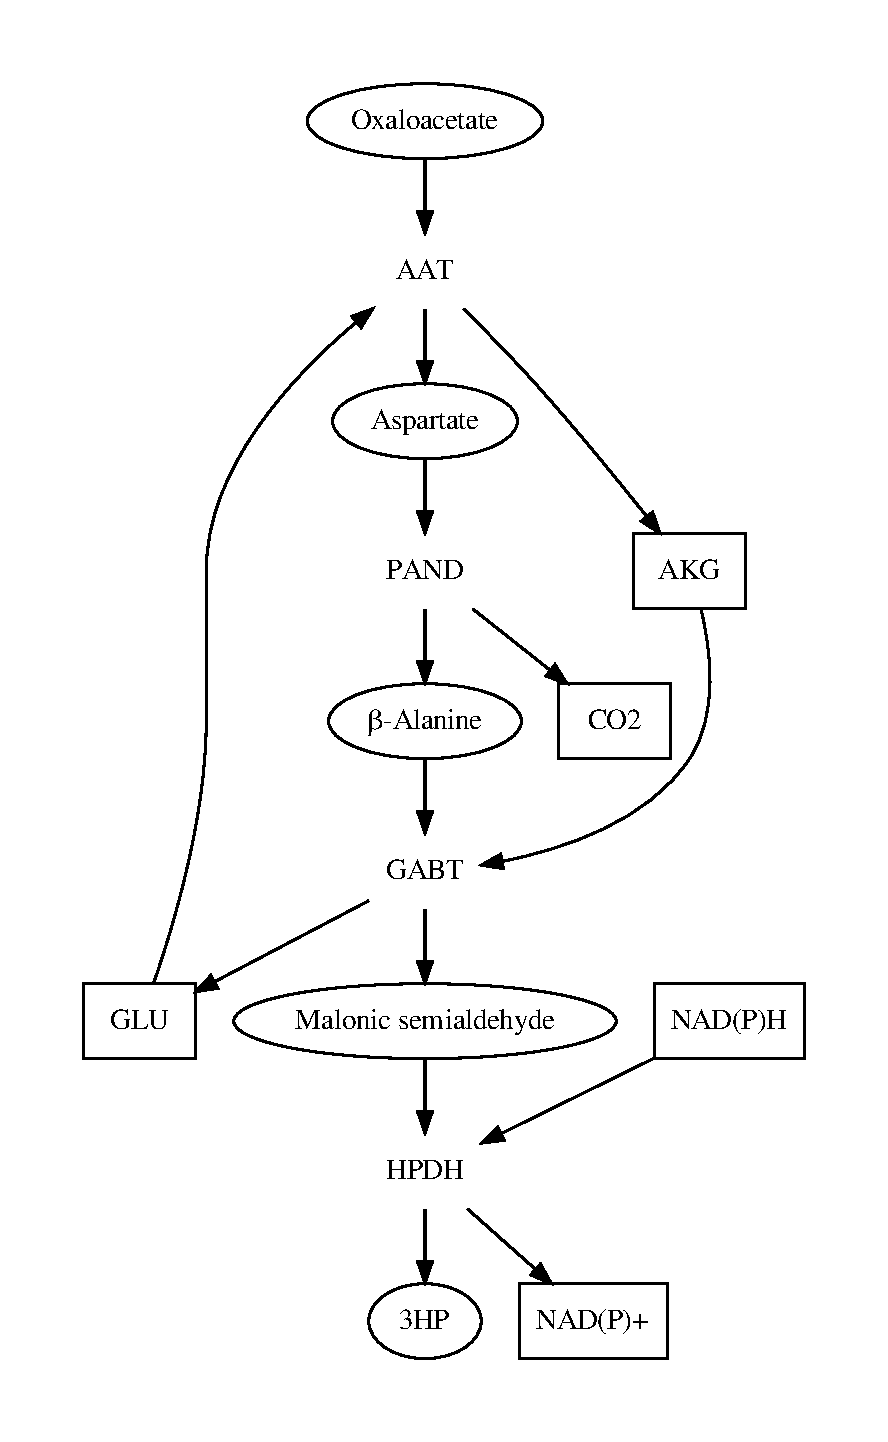
\includegraphics[max width=\linewidth, max height=0.5\paperheight]{2/new_pathway.pdf}
		\caption{The pathway to be added}
		\label{fig:pathway}
	\end{figure}
	We require the following additional metabolites:
	\begin{itemize}
		\item Aspartate, asp\_c
		\item $\beta$-Alanine, ala\_c
		\item Malonic Semaldehyde (3-Oxopropanoate), oxo\_c
		\item 3HP, hpa\_c
		\item L-Glutamate, glu\_c
	\end{itemize}
	and the following reactions:
	\begin{center}
	\begin{tabular}{r@{$\;\rightarrow\;$}l}
		oaa\_c + glu\_c & asp\_c + akg\_c \\
		asp\_c & ala\_c + co2\_c\\
		ala\_c + akg\_c & oxo\_c + glu\_c\\
		oxo\_c + nadph\_c & hpa\_c + nadp\_c\\
		hpa\_c & hpa\_e
	\end{tabular}
	\end{center}
	\subsection{Results}
		\begin{enumerate}[i)]
			\item Aerobic conditions yield ($\mathrm{\frac{ex\_hpa}{ex\_glc}}$): 0.09823718127269748
			\item Anaerobic conditions yield ($\mathrm{\frac{ex\_hpa}{ex\_glc}}$): 0.02415015570973515

		\end{enumerate}
		The pathway is active, and produces HPA, see the phaseplane in Figure \ref{fig:phaseplane}
		\begin{figure}[h]
			\centering
			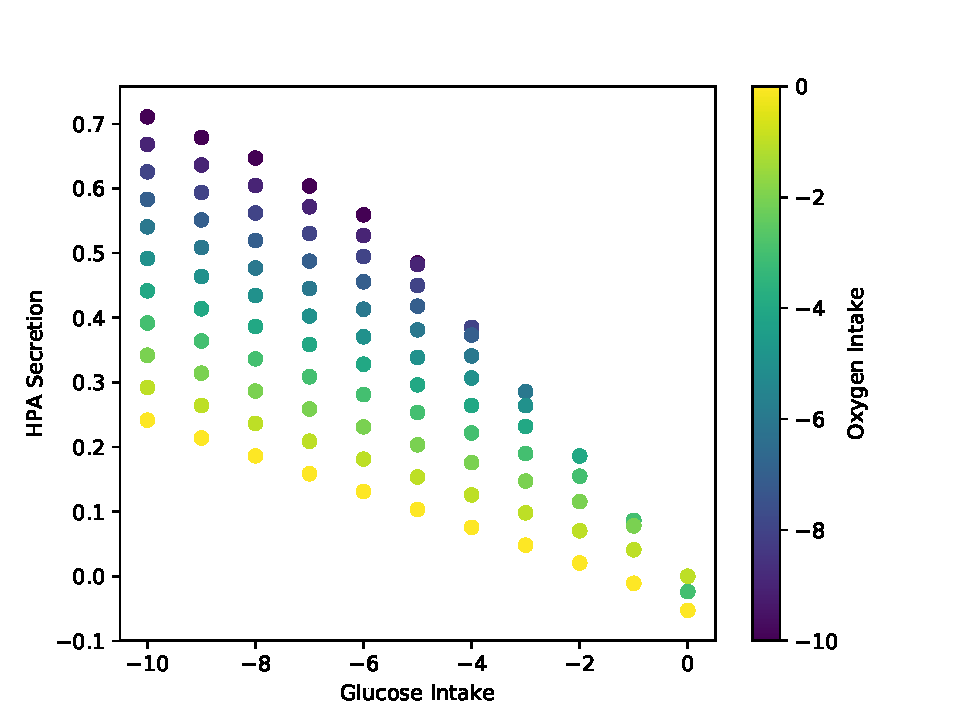
\includegraphics[max width=0.75\linewidth]{src/phaseplane.pdf}
			\caption{Phaseplane}
			\label{fig:phaseplane}
		\end{figure}
\section{Flux modulation}
	The flux modulation reveals the following ranges, with the non-overlapping ones coloured in red:
	\def\barplot#1#2{\tikz[baseline,x=0.02\linewidth,y=0.02\linewidth]{\begin{scope}[yshift=-0.25ex]\filldraw[thick, red]#1;\end{scope}\begin{scope}[yshift=0.25ex]\filldraw[thick, blue]#2;\end{scope} \path(-16.7,0) -- (29.15,0);\draw (0,-0.75ex) -- (0,0.75ex);}}
	\begin{longtable}{p{0.2\linewidth}p{0.8\linewidth}}
		\verb|DM_4CRSOL| & \barplot{0.0001}{0.0001}\\
\verb|DM_5DRIB| & \barplot{0.0002}{0.0002}\\
\verb|DM_AACALD| & \barplot{0.0000}{0.0000}\\
\verb|DM_AMOB| & \barplot{0.0000}{0.0000}\\
\verb|DM_MTHTHF| & \barplot{0.0001}{0.0001}\\
\verb|DM_OXAM| & \barplot{0.0000}{0.0000}\\
\verb|Ec_biomass_iJO1366_WT_53p95M| & \barplot{0.0000}{0.0000}\\
\verb|Ec_biomass_iJO1366_core_53p95M| & \barplot{0.2415}{0.2415}\\
\verb|EX_12ppd__R_e| & \barplot{0.0000}{0.0000}\\
\verb|EX_12ppd__S_e| & \barplot{0.0000}{0.0000}\\
\verb|EX_14glucan_e| & \barplot{0.0000}{0.0000}\\
\verb|EX_15dap_e| & \barplot{0.0000}{0.0000}\\
\verb|EX_23camp_e| & \barplot{0.0000}{0.0000}\\
\verb|EX_23ccmp_e| & \barplot{0.0000}{0.0000}\\
\verb|EX_23cgmp_e| & \barplot{0.0000}{0.0000}\\
\verb|EX_23cump_e| & \barplot{0.0000}{0.0000}\\
\verb|EX_23dappa_e| & \barplot{0.0000}{0.0000}\\
\verb|EX_26dap__M_e| & \barplot{0.0000}{0.0000}\\
\verb|EX_2ddglcn_e| & \barplot{0.0000}{0.0000}\\
\verb|EX_34dhpac_e| & \barplot{0.0000}{0.0000}\\
\verb|EX_3amp_e| & \barplot{0.0000}{0.0000}\\
\verb|EX_3cmp_e| & \barplot{0.0000}{0.0000}\\
\verb|EX_3gmp_e| & \barplot{0.0000}{0.0000}\\
\verb|EX_3hcinnm_e| & \barplot{0.0000}{0.0000}\\
\verb|EX_3hpp_e| & \barplot{0.0000}{0.0000}\\
\verb|EX_3hpppn_e| & \barplot{0.0000}{0.0000}\\
\verb|EX_3ump_e| & \barplot{0.0000}{0.0000}\\
\verb|EX_4abut_e| & \barplot{0.0000}{0.0000}\\
\verb|EX_4hoxpacd_e| & \barplot{0.0000}{0.0000}\\
\verb|EX_5dglcn_e| & \barplot{0.0000}{0.0000}\\
\verb|EX_5mtr_e| & \barplot{0.0000}{0.0000}\\
\verb|EX_LalaDglu_e| & \barplot{0.0000}{0.0000}\\
\verb|EX_LalaDgluMdap_e| & \barplot{0.0000}{0.0000}\\
\verb|EX_LalaDgluMdapDala_e| & \barplot{0.0000}{0.0000}\\
\verb|EX_LalaLglu_e| & \barplot{0.0000}{0.0000}\\
\verb|EX_ac_e| & \barplot{8.2076}{8.2076}\\
\verb|EX_acac_e| & \barplot{0.0000}{0.0000}\\
\verb|EX_acald_e| & \barplot{0.0000}{0.0000}\\
\verb|EX_acgal_e| & \barplot{0.0000}{0.0000}\\
\verb|EX_acgal1p_e| & \barplot{0.0000}{0.0000}\\
\verb|EX_acgam_e| & \barplot{0.0000}{0.0000}\\
\verb|EX_acgam1p_e| & \barplot{0.0000}{0.0000}\\
\verb|EX_acmana_e| & \barplot{0.0000}{0.0000}\\
\verb|EX_acmum_e| & \barplot{0.0000}{0.0000}\\
\verb|EX_acnam_e| & \barplot{0.0000}{0.0000}\\
\verb|EX_acolipa_e| & \barplot{0.0000}{0.0000}\\
\verb|EX_acser_e| & \barplot{0.0000}{0.0000}\\
\verb|EX_ade_e| & \barplot{0.0000}{0.0000}\\
\verb|EX_adn_e| & \barplot{0.0000}{0.0000}\\
\verb|EX_adocbl_e| & \barplot{0.0000}{0.0000}\\
\verb|EX_ag_e| & \barplot{0.0000}{0.0000}\\
\verb|EX_agm_e| & \barplot{0.0000}{0.0000}\\
\verb|EX_akg_e| & \barplot{0.0000}{0.0000}\\
\verb|EX_ala__B_e| & \barplot{0.0000}{0.0000}\\
\verb|EX_ala__D_e| & \barplot{0.0000}{0.0000}\\
\verb|EX_ala__L_e| & \barplot{0.0000}{0.0000}\\
\verb|EX_alaala_e| & \barplot{0.0000}{0.0000}\\
\verb|EX_all__D_e| & \barplot{0.0000}{0.0000}\\
\verb|EX_alltn_e| & \barplot{0.0000}{0.0000}\\
\verb|EX_amp_e| & \barplot{0.0000}{0.0000}\\
\verb|EX_anhgm_e| & \barplot{0.0000}{0.0000}\\
\verb|EX_arab__L_e| & \barplot{0.0000}{0.0000}\\
\verb|EX_arbt_e| & \barplot{0.0000}{0.0000}\\
\verb|EX_arbtn_e| & \barplot{0.0000}{0.0000}\\
\verb|EX_arbtn__fe3_e| & \barplot{0.0000}{0.0000}\\
\verb|EX_arg__L_e| & \barplot{0.0000}{0.0000}\\
\verb|EX_ascb__L_e| & \barplot{0.0000}{0.0000}\\
\verb|EX_asn__L_e| & \barplot{0.0000}{0.0000}\\
\verb|EX_aso3_e| & \barplot{0.0000}{0.0000}\\
\verb|EX_asp__L_e| & \barplot{0.0000}{0.0000}\\
\verb|EX_btn_e| & \barplot{0.0000}{0.0000}\\
\verb|EX_but_e| & \barplot{0.0000}{0.0000}\\
\verb|EX_butso3_e| & \barplot{0.0000}{-0.0000}\\
\verb|EX_ca2_e| & \barplot{-0.0013}{-0.0013}\\
\verb|EX_cbi_e| & \barplot{0.0000}{0.0000}\\
\verb|EX_cbl1_e| & \barplot{0.0000}{-0.0000}\\
\verb|EX_cd2_e| & \barplot{0.0000}{0.0000}\\
\verb|EX_cgly_e| & \barplot{0.0000}{0.0000}\\
\verb|EX_chol_e| & \barplot{0.0000}{0.0000}\\
\verb|EX_chtbs_e| & \barplot{0.0000}{0.0000}\\
\verb|EX_cit_e| & \barplot{0.0000}{0.0000}\\
\verb|EX_cl_e| & \barplot{-0.0013}{-0.0013}\\
\verb|EX_cm_e| & \barplot{0.0000}{0.0000}\\
\verb|EX_cmp_e| & \barplot{0.0000}{0.0000}\\
\verb|EX_co2_e| & \barplot{-0.0882}{-0.0882}\\
\verb|EX_cobalt2_e| & \barplot{-0.0000}{-0.0000}\\
\verb|EX_colipa_e| & \barplot{0.0000}{0.0000}\\
\verb|EX_colipap_e| & \barplot{0.0000}{0.0000}\\
\verb|EX_cpgn_e| & \barplot{0.0000}{0.0000}\\
\verb|EX_cpgn__un_e| & \barplot{0.0000}{0.0000}\\
\verb|EX_crn_e| & \barplot{0.0000}{0.0000}\\
\verb|EX_crn__D_e| & \barplot{0.0000}{0.0000}\\
\verb|EX_csn_e| & \barplot{0.0000}{0.0000}\\
\verb|EX_cu_e| & \barplot{0.0000}{0.0000}\\
\verb|EX_cu2_e| & \barplot{-0.0002}{-0.0002}\\
\verb|EX_cyan_e| & \barplot{0.0000}{0.0000}\\
\verb|EX_cynt_e| & \barplot{0.0000}{0.0000}\\
\verb|EX_cys__D_e| & \barplot{0.0000}{0.0000}\\
\verb|EX_cys__L_e| & \barplot{0.0000}{0.0000}\\
\verb|EX_cytd_e| & \barplot{0.0000}{0.0000}\\
\verb|EX_dad__2_e| & \barplot{0.0000}{0.0000}\\
\verb|EX_damp_e| & \barplot{0.0000}{0.0000}\\
\verb|EX_dca_e| & \barplot{0.0000}{0.0000}\\
\verb|EX_dcmp_e| & \barplot{0.0000}{0.0000}\\
\verb|EX_dcyt_e| & \barplot{0.0000}{0.0000}\\
\verb|EX_ddca_e| & \barplot{0.0000}{0.0000}\\
\verb|EX_dgmp_e| & \barplot{0.0000}{0.0000}\\
\verb|EX_dgsn_e| & \barplot{0.0000}{0.0000}\\
\verb|EX_dha_e| & \barplot{0.0000}{0.0000}\\
\verb|EX_dimp_e| & \barplot{0.0000}{0.0000}\\
\verb|EX_din_e| & \barplot{0.0000}{0.0000}\\
\verb|EX_dms_e| & \barplot{0.0000}{0.0000}\\
\verb|EX_dmso_e| & \barplot{0.0000}{0.0000}\\
\verb|EX_dopa_e| & \barplot{0.0000}{0.0000}\\
\verb|EX_doxrbcn_e| & \barplot{0.0000}{0.0000}\\
\verb|EX_dtmp_e| & \barplot{0.0000}{0.0000}\\
\verb|EX_dump_e| & \barplot{0.0000}{0.0000}\\
\verb|EX_duri_e| & \barplot{0.0000}{0.0000}\\
\verb|EX_eca4colipa_e| & \barplot{0.0000}{0.0000}\\
\verb|EX_enlipa_e| & \barplot{0.0000}{0.0000}\\
\verb|EX_enter_e| & \barplot{0.0000}{0.0000}\\
\verb|EX_etha_e| & \barplot{0.0000}{0.0000}\\
\verb|EX_ethso3_e| & \barplot{0.0000}{0.0000}\\
\verb|EX_etoh_e| & \barplot{8.0777}{8.0777}\\
\verb|EX_f6p_e| & \barplot{0.0000}{0.0000}\\
\verb|EX_fald_e| & \barplot{0.0000}{0.0000}\\
\verb|EX_fe2_e| & \barplot{-0.0020}{-0.0020}\\
\verb|EX_fe3_e| & \barplot{-0.0019}{-0.0019}\\
\verb|EX_fe3dcit_e| & \barplot{0.0000}{0.0000}\\
\verb|EX_fe3dhbzs_e| & \barplot{0.0000}{0.0000}\\
\verb|EX_fe3hox_e| & \barplot{0.0000}{0.0000}\\
\verb|EX_fe3hox__un_e| & \barplot{0.0000}{0.0000}\\
\verb|EX_fecrm_e| & \barplot{0.0000}{0.0000}\\
\verb|EX_fecrm__un_e| & \barplot{0.0000}{0.0000}\\
\verb|EX_feenter_e| & \barplot{0.0000}{0.0000}\\
\verb|EX_feoxam_e| & \barplot{0.0000}{0.0000}\\
\verb|EX_feoxam__un_e| & \barplot{0.0000}{0.0000}\\
\verb|EX_for_e| & \barplot{17.2833}{17.2833}\\
\verb|EX_fru_e| & \barplot{0.0000}{0.0000}\\
\verb|EX_frulys_e| & \barplot{0.0000}{0.0000}\\
\verb|EX_fruur_e| & \barplot{0.0000}{0.0000}\\
\verb|EX_fuc__L_e| & \barplot{0.0000}{0.0000}\\
\verb|EX_fum_e| & \barplot{0.0000}{0.0000}\\
\verb|EX_fusa_e| & \barplot{0.0000}{0.0000}\\
\verb|EX_g1p_e| & \barplot{0.0000}{0.0000}\\
\verb|EX_g3pc_e| & \barplot{-0.0000}{0.0000}\\
\verb|EX_g3pe_e| & \barplot{0.0000}{0.0000}\\
\verb|EX_g3pg_e| & \barplot{0.0000}{0.0000}\\
\verb|EX_g3pi_e| & \barplot{0.0000}{0.0000}\\
\verb|EX_g3ps_e| & \barplot{0.0000}{0.0000}\\
\verb|EX_g6p_e| & \barplot{0.0000}{0.0000}\\
\verb|EX_gal_e| & \barplot{0.0000}{0.0000}\\
\verb|EX_gal__bD_e| & \barplot{0.0000}{0.0000}\\
\verb|EX_gal1p_e| & \barplot{0.0000}{0.0000}\\
\verb|EX_galct__D_e| & \barplot{0.0000}{0.0000}\\
\verb|EX_galctn__D_e| & \barplot{0.0000}{0.0000}\\
\verb|EX_galctn__L_e| & \barplot{0.0000}{0.0000}\\
\verb|EX_galt_e| & \barplot{0.0000}{0.0000}\\
\verb|EX_galur_e| & \barplot{0.0000}{0.0000}\\
\verb|EX_gam_e| & \barplot{0.0000}{0.0000}\\
\verb|EX_gam6p_e| & \barplot{0.0000}{0.0000}\\
\verb|EX_gbbtn_e| & \barplot{0.0000}{0.0000}\\
\verb|EX_gdp_e| & \barplot{0.0000}{0.0000}\\
\verb|EX_glc_e| & \barplot{-10.0000}{-10.0000}\\
\verb|EX_glcn_e| & \barplot{0.0000}{0.0000}\\
\verb|EX_glcr_e| & \barplot{0.0000}{0.0000}\\
\verb|EX_glcur_e| & \barplot{0.0000}{0.0000}\\
\verb|EX_glcur1p_e| & \barplot{0.0000}{0.0000}\\
\verb|EX_gln__L_e| & \barplot{0.0000}{0.0000}\\
\verb|EX_glu__L_e| & \barplot{0.0000}{0.0000}\\
\verb|EX_gly_e| & \barplot{0.0000}{0.0000}\\
\verb|EX_glyald_e| & \barplot{0.0000}{0.0000}\\
\verb|EX_glyb_e| & \barplot{0.0000}{0.0000}\\
\verb|EX_glyc_e| & \barplot{0.0000}{0.0000}\\
\verb|EX_glyc__R_e| & \barplot{0.0000}{0.0000}\\
\verb|EX_glyc2p_e| & \barplot{0.0000}{0.0000}\\
\verb|EX_glyc3p_e| & \barplot{0.0000}{0.0000}\\
\verb|EX_glyclt_e| & \barplot{0.0002}{0.0002}\\
\verb|EX_gmp_e| & \barplot{0.0000}{0.0000}\\
\verb|EX_gsn_e| & \barplot{0.0000}{0.0000}\\
\verb|EX_gthox_e| & \barplot{0.0000}{0.0000}\\
\verb|EX_gthrd_e| & \barplot{0.0000}{0.0000}\\
\verb|EX_gtp_e| & \barplot{0.0000}{0.0000}\\
\verb|EX_gua_e| & \barplot{0.0000}{0.0000}\\
\verb|EX_h_e| & \barplot{27.8721}{27.8721}\\
\verb|EX_h2_e| & \barplot{0.0000}{0.0000}\\
\verb|EX_h2o_e| & \barplot{-1.7088}{-1.7088}\\
\verb|EX_h2o2_e| & \barplot{0.0000}{0.0000}\\
\verb|EX_h2s_e| & \barplot{0.0000}{0.0000}\\
\verb|EX_hacolipa_e| & \barplot{0.0000}{0.0000}\\
\verb|EX_halipa_e| & \barplot{0.0000}{0.0000}\\
\verb|EX_hdca_e| & \barplot{0.0000}{0.0000}\\
\verb|EX_hdcea_e| & \barplot{0.0000}{0.0000}\\
\verb|EX_hg2_e| & \barplot{0.0000}{0.0000}\\
\verb|EX_his__L_e| & \barplot{0.0000}{0.0000}\\
\verb|EX_hom__L_e| & \barplot{0.0000}{0.0000}\\
\verb|EX_hxa_e| & \barplot{0.0000}{0.0000}\\
\verb|EX_hxan_e| & \barplot{0.0000}{0.0000}\\
\verb|EX_idon__L_e| & \barplot{0.0000}{0.0000}\\
\verb|EX_ile__L_e| & \barplot{0.0000}{0.0000}\\
\verb|EX_imp_e| & \barplot{0.0000}{0.0000}\\
\verb|EX_indole_e| & \barplot{0.0000}{0.0000}\\
\verb|EX_inost_e| & \barplot{0.0000}{0.0000}\\
\verb|EX_ins_e| & \barplot{0.0000}{0.0000}\\
\verb|EX_isetac_e| & \barplot{0.0000}{-0.0000}\\
\verb|EX_k_e| & \barplot{-0.0471}{-0.0471}\\
\verb|EX_kdo2lipid4_e| & \barplot{0.0000}{0.0000}\\
\verb|EX_lac__D_e| & \barplot{0.0000}{0.0000}\\
\verb|EX_lac__L_e| & \barplot{0.0000}{0.0000}\\
\verb|EX_lcts_e| & \barplot{0.0000}{0.0000}\\
\verb|EX_leu__L_e| & \barplot{0.0000}{0.0000}\\
\verb|EX_lipa_e| & \barplot{0.0000}{0.0000}\\
\verb|EX_lipa_cold_e| & \barplot{0.0000}{0.0000}\\
\verb|EX_lipoate_e| & \barplot{0.0000}{0.0000}\\
\verb|EX_lys__L_e| & \barplot{-0.0000}{0.0000}\\
\verb|EX_lyx__L_e| & \barplot{0.0000}{0.0000}\\
\verb|EX_mal__D_e| & \barplot{0.0000}{0.0000}\\
\verb|EX_mal__L_e| & \barplot{-0.0000}{0.0000}\\
\verb|EX_malt_e| & \barplot{-0.0000}{0.0000}\\
\verb|EX_malthx_e| & \barplot{-0.0000}{0.0000}\\
\verb|EX_maltpt_e| & \barplot{0.0000}{0.0000}\\
\verb|EX_malttr_e| & \barplot{0.0000}{0.0000}\\
\verb|EX_maltttr_e| & \barplot{0.0000}{0.0000}\\
\verb|EX_man_e| & \barplot{0.0000}{0.0000}\\
\verb|EX_man6p_e| & \barplot{0.0000}{0.0000}\\
\verb|EX_manglyc_e| & \barplot{0.0000}{0.0000}\\
\verb|EX_melib_e| & \barplot{0.0000}{0.0000}\\
\verb|EX_meoh_e| & \barplot{0.0000}{0.0000}\\
\verb|EX_met__D_e| & \barplot{0.0000}{0.0000}\\
\verb|EX_met__L_e| & \barplot{0.0000}{0.0000}\\
\verb|EX_metsox__R__L_e| & \barplot{0.0000}{0.0000}\\
\verb|EX_metsox__S__L_e| & \barplot{0.0000}{0.0000}\\
\verb|EX_mg2_e| & \barplot{-0.0021}{-0.0021}\\
\verb|EX_mincyc_e| & \barplot{0.0000}{0.0000}\\
\verb|EX_minohp_e| & \barplot{0.0000}{0.0000}\\
\verb|EX_mmet_e| & \barplot{0.0000}{0.0000}\\
\verb|EX_mn2_e| & \barplot{-0.0002}{-0.0002}\\
\verb|EX_mnl_e| & \barplot{0.0000}{0.0000}\\
\verb|EX_mobd_e| & \barplot{-0.0000}{-0.0000}\\
\verb|EX_mso3_e| & \barplot{0.0000}{0.0000}\\
\verb|EX_n2o_e| & \barplot{0.0000}{0.0000}\\
\verb|EX_na1_e| & \barplot{0.0000}{0.0000}\\
\verb|EX_nac_e| & \barplot{0.0000}{0.0000}\\
\verb|EX_nh4_e| & \barplot{-2.6084}{-2.6084}\\
\verb|EX_ni2_e| & \barplot{-0.0001}{-0.0001}\\
\verb|EX_nmn_e| & \barplot{0.0000}{0.0000}\\
\verb|EX_no_e| & \barplot{0.0000}{0.0000}\\
\verb|EX_no2_e| & \barplot{0.0000}{0.0000}\\
\verb|EX_no3_e| & \barplot{0.0000}{0.0000}\\
\verb|EX_novbcn_e| & \barplot{0.0000}{0.0000}\\
\verb|EX_o16a4colipa_e| & \barplot{0.0000}{0.0000}\\
\verb|EX_o2_e| & \barplot{0.0000}{0.0000}\\
\verb|EX_o2s_e| & \barplot{0.0000}{0.0000}\\
\verb|EX_ocdca_e| & \barplot{0.0000}{0.0000}\\
\verb|EX_ocdcea_e| & \barplot{0.0000}{0.0000}\\
\verb|EX_octa_e| & \barplot{0.0000}{0.0000}\\
\verb|EX_orn_e| & \barplot{0.0000}{0.0000}\\
\verb|EX_orot_e| & \barplot{0.0000}{0.0000}\\
\verb|EX_pacald_e| & \barplot{0.0000}{0.0000}\\
\verb|EX_peamn_e| & \barplot{0.0000}{0.0000}\\
\verb|EX_phe__L_e| & \barplot{0.0000}{0.0000}\\
\verb|EX_pheme_e| & \barplot{0.0000}{0.0000}\\
\verb|EX_pi_e| & \barplot{-0.2330}{-0.2330}\\
\verb|EX_pnto__R_e| & \barplot{0.0000}{0.0000}\\
\verb|EX_ppa_e| & \barplot{0.0000}{0.0000}\\
\verb|EX_ppal_e| & \barplot{0.0000}{0.0000}\\
\verb|EX_pppn_e| & \barplot{0.0000}{0.0000}\\
\verb|EX_ppt_e| & \barplot{0.0000}{0.0000}\\
\verb|EX_pro__L_e| & \barplot{0.0000}{0.0000}\\
\verb|EX_progly_e| & \barplot{-0.0000}{0.0000}\\
\verb|EX_psclys_e| & \barplot{-0.0000}{0.0000}\\
\verb|EX_pser__L_e| & \barplot{0.0000}{0.0000}\\
\verb|EX_ptrc_e| & \barplot{0.0000}{0.0000}\\
\verb|EX_pydam_e| & \barplot{0.0000}{0.0000}\\
\verb|EX_pydx_e| & \barplot{0.0000}{0.0000}\\
\verb|EX_pydxn_e| & \barplot{0.0000}{0.0000}\\
\verb|EX_pyr_e| & \barplot{0.0000}{0.0000}\\
\verb|EX_quin_e| & \barplot{0.0000}{0.0000}\\
\verb|EX_r5p_e| & \barplot{0.0000}{0.0000}\\
\verb|EX_rfamp_e| & \barplot{0.0000}{0.0000}\\
\verb|EX_rib__D_e| & \barplot{0.0000}{0.0000}\\
\verb|EX_rmn_e| & \barplot{0.0000}{0.0000}\\
\verb|EX_sbt__D_e| & \barplot{0.0000}{0.0000}\\
\verb|EX_sel_e| & \barplot{0.0000}{0.0000}\\
\verb|EX_ser__D_e| & \barplot{0.0000}{0.0000}\\
\verb|EX_ser__L_e| & \barplot{0.0000}{0.0000}\\
\verb|EX_skm_e| & \barplot{0.0000}{0.0000}\\
\verb|EX_slnt_e| & \barplot{0.0000}{0.0000}\\
\verb|EX_so2_e| & \barplot{0.0000}{0.0000}\\
\verb|EX_so3_e| & \barplot{0.0000}{0.0000}\\
\verb|EX_so4_e| & \barplot{-0.0609}{-0.0609}\\
\verb|EX_spmd_e| & \barplot{0.0000}{0.0000}\\
\verb|EX_succ_e| & \barplot{0.0800}{0.0800}\\
\verb|EX_sucr_e| & \barplot{0.0000}{0.0000}\\
\verb|EX_sulfac_e| & \barplot{0.0000}{-0.0000}\\
\verb|EX_tartr__D_e| & \barplot{0.0000}{0.0000}\\
\verb|EX_tartr__L_e| & \barplot{0.0000}{0.0000}\\
\verb|EX_taur_e| & \barplot{0.0000}{-0.0000}\\
\verb|EX_tcynt_e| & \barplot{0.0000}{0.0000}\\
\verb|EX_thm_e| & \barplot{0.0000}{0.0000}\\
\verb|EX_thr__L_e| & \barplot{0.0000}{0.0000}\\
\verb|EX_thrp_e| & \barplot{0.0000}{0.0000}\\
\verb|EX_thym_e| & \barplot{0.0000}{0.0000}\\
\verb|EX_thymd_e| & \barplot{0.0000}{0.0000}\\
\verb|EX_tma_e| & \barplot{0.0000}{0.0000}\\
\verb|EX_tmao_e| & \barplot{0.0000}{0.0000}\\
\verb|EX_tre_e| & \barplot{0.0000}{0.0000}\\
\verb|EX_trp__L_e| & \barplot{0.0000}{0.0000}\\
\verb|EX_tsul_e| & \barplot{0.0000}{0.0000}\\
\verb|EX_ttdca_e| & \barplot{0.0000}{0.0000}\\
\verb|EX_ttdcea_e| & \barplot{0.0000}{0.0000}\\
\verb|EX_ttrcyc_e| & \barplot{0.0000}{0.0000}\\
\verb|EX_tungs_e| & \barplot{0.0000}{0.0000}\\
\verb|EX_tym_e| & \barplot{0.0000}{0.0000}\\
\verb|EX_tyr__L_e| & \barplot{0.0000}{0.0000}\\
\verb|EX_tyrp_e| & \barplot{0.0000}{0.0000}\\
\verb|EX_uacgam_e| & \barplot{0.0000}{0.0000}\\
\verb|EX_udpacgal_e| & \barplot{0.0000}{0.0000}\\
\verb|EX_udpg_e| & \barplot{0.0000}{0.0000}\\
\verb|EX_udpgal_e| & \barplot{-0.0000}{0.0000}\\
\verb|EX_udpglcur_e| & \barplot{0.0000}{0.0000}\\
\verb|EX_ump_e| & \barplot{0.0000}{0.0000}\\
\verb|EX_ura_e| & \barplot{0.0000}{0.0000}\\
\verb|EX_urea_e| & \barplot{0.0000}{0.0000}\\
\verb|EX_uri_e| & \barplot{0.0000}{0.0000}\\
\verb|EX_val__L_e| & \barplot{0.0000}{0.0000}\\
\verb|EX_xan_e| & \barplot{0.0000}{0.0000}\\
\verb|EX_xmp_e| & \barplot{0.0000}{0.0000}\\
\verb|EX_xtsn_e| & \barplot{0.0000}{0.0000}\\
\verb|EX_xyl__D_e| & \barplot{0.0000}{0.0000}\\
\verb|EX_xylu__L_e| & \barplot{0.0000}{0.0000}\\
\verb|EX_zn2_e| & \barplot{-0.0001}{-0.0001}\\
\verb|12DGR120tipp| & \barplot{0.0000}{0.0000}\\
\verb|12DGR140tipp| & \barplot{0.0000}{0.0000}\\
\verb|12DGR141tipp| & \barplot{0.0000}{0.0000}\\
\verb|12DGR160tipp| & \barplot{0.0000}{0.0000}\\
\verb|12DGR161tipp| & \barplot{0.0000}{0.0000}\\
\verb|12DGR180tipp| & \barplot{0.0000}{0.0000}\\
\verb|12DGR181tipp| & \barplot{0.0000}{0.0000}\\
\verb|12PPDRtex| & \barplot{0.0000}{-0.0000}\\
\verb|12PPDRtpp| & \barplot{0.0000}{-0.0000}\\
\verb|12PPDStex| & \barplot{0.0000}{-0.0000}\\
\verb|12PPDStpp| & \barplot{0.0000}{-0.0000}\\
\verb|14GLUCANabcpp| & \barplot{0.0000}{0.0000}\\
\verb|14GLUCANtexi| & \barplot{0.0000}{-0.0000}\\
\verb|23CAMPtex| & \barplot{0.0000}{0.0000}\\
\verb|23CCMPtex| & \barplot{0.0000}{0.0000}\\
\verb|23CGMPtex| & \barplot{0.0000}{-0.0000}\\
\verb|23CUMPtex| & \barplot{0.0000}{0.0000}\\
\verb|23DAPPAt2pp| & \barplot{0.0000}{0.0000}\\
\verb|23DAPPAtex| & \barplot{0.0000}{0.0000}\\
\verb|23PDE2pp| & \barplot{0.0000}{0.0000}\\
\verb|23PDE4pp| & \barplot{0.0000}{0.0000}\\
\verb|23PDE7pp| & \barplot{0.0000}{0.0000}\\
\verb|23PDE9pp| & \barplot{0.0000}{-0.0000}\\
\verb|26DAHtex| & \barplot{0.0000}{0.0000}\\
\verb|2AGPA120tipp| & \barplot{0.0000}{0.0000}\\
\verb|2AGPA140tipp| & \barplot{0.0000}{0.0000}\\
\verb|2AGPA141tipp| & \barplot{0.0000}{0.0000}\\
\verb|2AGPA160tipp| & \barplot{0.0000}{0.0000}\\
\verb|2AGPA161tipp| & \barplot{0.0000}{0.0000}\\
\verb|2AGPA180tipp| & \barplot{0.0000}{0.0000}\\
\verb|2AGPA181tipp| & \barplot{0.0000}{0.0000}\\
\verb|2AGPE120tipp| & \barplot{0.0000}{0.0000}\\
\verb|2AGPE140tipp| & \barplot{0.0000}{0.0000}\\
\verb|2AGPE141tipp| & \barplot{0.0000}{0.0000}\\
\verb|2AGPE160tipp| & \barplot{0.0000}{0.0000}\\
\verb|2AGPE161tipp| & \barplot{0.0000}{0.0000}\\
\verb|2AGPE180tipp| & \barplot{0.0000}{0.0000}\\
\verb|2AGPE181tipp| & \barplot{0.0000}{0.0000}\\
\verb|2AGPEAT120| & \barplot{0.0000}{0.0000}\\
\verb|2AGPEAT140| & \barplot{0.0000}{0.0000}\\
\verb|2AGPEAT141| & \barplot{0.0000}{0.0000}\\
\verb|2AGPEAT160| & \barplot{0.0000}{0.0000}\\
\verb|2AGPEAT161| & \barplot{0.0000}{0.0000}\\
\verb|2AGPEAT180| & \barplot{0.0000}{0.0000}\\
\verb|2AGPEAT181| & \barplot{0.0000}{0.0000}\\
\verb|2AGPG120tipp| & \barplot{0.0000}{0.0000}\\
\verb|2AGPG140tipp| & \barplot{0.0000}{0.0000}\\
\verb|2AGPG141tipp| & \barplot{0.0000}{0.0000}\\
\verb|2AGPG160tipp| & \barplot{0.0000}{0.0000}\\
\verb|2AGPG161tipp| & \barplot{0.0000}{0.0000}\\
\verb|2AGPG180tipp| & \barplot{0.0000}{0.0000}\\
\verb|2AGPG181tipp| & \barplot{0.0000}{0.0000}\\
\verb|2AGPGAT120| & \barplot{0.0000}{0.0000}\\
\verb|2AGPGAT140| & \barplot{0.0000}{0.0000}\\
\verb|2AGPGAT141| & \barplot{0.0000}{0.0000}\\
\verb|2AGPGAT160| & \barplot{0.0000}{0.0000}\\
\verb|2AGPGAT161| & \barplot{0.0000}{0.0000}\\
\verb|2AGPGAT180| & \barplot{0.0000}{0.0000}\\
\verb|2AGPGAT181| & \barplot{0.0000}{0.0000}\\
\verb|2DGULRGx| & \barplot{0.0000}{0.0000}\\
\verb|2DGULRGy| & \barplot{0.0000}{0.0000}\\
\verb|2DGULRx| & \barplot{0.0000}{0.0000}\\
\verb|2DGULRy| & \barplot{0.0000}{0.0000}\\
\verb|2MAHMP| & \barplot{0.0000}{0.0000}\\
\verb|34dhpactex| & \barplot{0.0000}{0.0000}\\
\verb|3AMACHYD| & \barplot{0.0000}{0.0000}\\
\verb|3AMPtex| & \barplot{0.0000}{0.0000}\\
\verb|3CMPtex| & \barplot{0.0000}{0.0000}\\
\verb|3GMPtex| & \barplot{0.0000}{-0.0000}\\
\verb|3HAD100| & \barplot{0.0000}{0.0000}\\
\verb|3HAD120| & \barplot{0.0000}{0.0000}\\
\verb|3HAD121| & \barplot{0.0000}{0.0000}\\
\verb|3HAD140| & \barplot{0.0000}{0.0000}\\
\verb|3HAD141| & \barplot{0.0000}{0.0000}\\
\verb|3HAD160| & \barplot{0.0000}{0.0000}\\
\verb|3HAD161| & \barplot{0.0000}{0.0000}\\
\verb|3HAD180| & \barplot{0.0000}{0.0000}\\
\verb|3HAD181| & \barplot{0.0000}{0.0000}\\
\verb|3HAD40| & \barplot{0.0000}{0.0000}\\
\verb|3HAD60| & \barplot{0.0000}{0.0000}\\
\verb|3HAD80| & \barplot{0.0000}{0.0000}\\
\verb|3HCINNMH| & \barplot{0.0000}{0.0000}\\
\verb|3HPPPNH| & \barplot{0.0000}{0.0000}\\
\verb|3HPPtex| & \barplot{-0.0000}{0.0000}\\
\verb|3HPPtpp| & \barplot{-0.0000}{0.0000}\\
\verb|3KGK| & \barplot{0.0000}{0.0000}\\
\verb|3NTD2pp| & \barplot{0.0000}{0.0000}\\
\verb|3NTD4pp| & \barplot{0.0000}{0.0000}\\
\verb|3NTD7pp| & \barplot{0.0000}{0.0000}\\
\verb|3NTD9pp| & \barplot{0.0000}{0.0000}\\
\verb|3OAR100| & \barplot{0.0000}{0.0000}\\
\verb|3OAR120| & \barplot{0.0000}{0.0000}\\
\verb|3OAR121| & \barplot{0.0000}{0.0000}\\
\verb|3OAR140| & \barplot{0.0188}{0.0188}\\
\verb|3OAR141| & \barplot{0.0000}{0.0000}\\
\verb|3OAR160| & \barplot{0.0000}{0.0000}\\
\verb|3OAR161| & \barplot{0.0000}{0.0000}\\
\verb|3OAR180| & \barplot{0.0000}{0.0000}\\
\verb|3OAR181| & \barplot{0.0000}{0.0000}\\
\verb|3OAR40| & \barplot{0.0000}{0.0000}\\
\verb|3OAR60| & \barplot{0.0000}{0.0000}\\
\verb|3OAR80| & \barplot{0.0000}{0.0000}\\
\verb|3OAS100| & \barplot{0.0000}{0.0000}\\
\verb|3OAS120| & \barplot{0.0000}{0.0000}\\
\verb|3OAS121| & \barplot{0.0000}{0.0000}\\
\verb|3OAS140| & \barplot{0.0188}{0.0188}\\
\verb|3OAS141| & \barplot{0.0000}{0.0000}\\
\verb|3OAS160| & \barplot{0.0000}{0.0000}\\
\verb|3OAS161| & \barplot{0.0000}{0.0000}\\
\verb|3OAS180| & \barplot{0.0000}{0.0000}\\
\verb|3OAS181| & \barplot{0.0000}{0.0000}\\
\verb|3OAS60| & \barplot{0.0000}{0.0000}\\
\verb|3OAS80| & \barplot{0.0000}{0.0000}\\
\verb|3OXCOAT| & \barplot{0.0000}{0.0000}\\
\verb|3PEPTabcpp| & \barplot{0.0000}{0.0000}\\
\verb|3PEPTtex| & \barplot{0.0000}{-0.0000}\\
\verb|3UMPtex| & \barplot{0.0000}{0.0000}\\
\verb|42A12BOOXpp| & \barplot{0.0000}{0.0000}\\
\verb|4HOXPACDtex| & \barplot{0.0000}{0.0000}\\
\verb|4HTHRS| & \barplot{0.0000}{0.0000}\\
\verb|4PCP| & \barplot{0.0000}{0.0000}\\
\verb|4PCPpp| & \barplot{0.0000}{0.0000}\\
\verb|4PEPTabcpp| & \barplot{0.0000}{0.0000}\\
\verb|4PEPTtex| & \barplot{0.0000}{-0.0000}\\
\verb|5DGLCNR| & \barplot{0.0000}{-0.0000}\\
\verb|5DGLCNt2rpp| & \barplot{0.0000}{-0.0000}\\
\verb|5DGLCNtex| & \barplot{0.0000}{-0.0000}\\
\verb|5DOAN| & \barplot{0.0002}{0.0002}\\
\verb|5MTRtex| & \barplot{0.0000}{-0.0000}\\
\verb|5MTRtpp| & \barplot{0.0000}{-0.0000}\\
\verb|A5PISO| & \barplot{0.0094}{0.0094}\\
\verb|AACPS1| & \barplot{0.0000}{0.0000}\\
\verb|AACPS2| & \barplot{0.0000}{0.0000}\\
\verb|AACPS3| & \barplot{0.0308}{0.0308}\\
\verb|AACPS4| & \barplot{0.0363}{0.0363}\\
\verb|AACPS5| & \barplot{0.0000}{0.0000}\\
\verb|AACPS6| & \barplot{0.0000}{0.0000}\\
\verb|AACPS7| & \barplot{0.0188}{0.0188}\\
\verb|AACPS8| & \barplot{0.0000}{0.0000}\\
\verb|AACPS9| & \barplot{0.0000}{0.0000}\\
\verb|AACTOOR| & \barplot{0.0000}{0.0000}\\
\verb|AADDGT| & \barplot{0.0000}{0.0000}\\
\verb|AAMYL| & \barplot{0.0000}{0.0000}\\
\verb|AAMYLpp| & \barplot{0.0000}{0.0000}\\
\verb|AB6PGH| & \barplot{0.0000}{0.0000}\\
\verb|ABTA| & \barplot{0.0000}{0.0000}\\
\verb|ABUTD| & \barplot{0.0000}{0.0000}\\
\verb|ABUTt2pp| & \barplot{35.0000}{0.0000}\\
\verb|ABUTtex| & \barplot{0.0000}{-0.0000}\\
\verb|ACACCT| & \barplot{0.0000}{0.0000}\\
\verb|ACACT1r| & \barplot{0.0859}{0.0859}\\
\verb|ACACT2r| & \barplot{0.0859}{0.0859}\\
\verb|ACACT3r| & \barplot{0.0859}{0.0859}\\
\verb|ACACT4r| & \barplot{0.0859}{0.0859}\\
\verb|ACACT5r| & \barplot{0.0859}{0.0859}\\
\verb|ACACT6r| & \barplot{0.0672}{0.0672}\\
\verb|ACACT7r| & \barplot{0.0672}{0.0672}\\
\verb|ACACT8r| & \barplot{0.0000}{-0.0000}\\
\verb|ACACt2pp| & \barplot{0.0000}{0.0000}\\
\verb|ACACtex| & \barplot{0.0000}{0.0000}\\
\verb|ACALD| & \barplot{-8.0777}{-8.0777}\\
\verb|ACALDtex| & \barplot{0.0000}{-0.0000}\\
\verb|ACALDtpp| & \barplot{0.0000}{-0.0000}\\
\verb|ACANTHAT| & \barplot{-0.0000}{0.0000}\\
\verb|ACBIPGT| & \barplot{0.0000}{0.0000}\\
\verb|ACCOAC| & \barplot{0.0188}{0.0188}\\
\verb|ACCOAL| & \barplot{35.0000}{0.0000}\\
\verb|ACGAL1PPpp| & \barplot{0.0000}{0.0000}\\
\verb|ACGAL1Ptex| & \barplot{0.0000}{0.0000}\\
\verb|ACGALtex| & \barplot{0.0000}{0.0000}\\
\verb|ACGAM1PPpp| & \barplot{0.0000}{-0.0000}\\
\verb|ACGAM1Ptex| & \barplot{0.0000}{-0.0000}\\
\verb|ACGAMK| & \barplot{0.0000}{0.0000}\\
\verb|ACGAMT| & \barplot{0.0000}{0.0000}\\
\verb|ACGAptspp| & \barplot{0.0000}{0.0000}\\
\verb|ACGAtex| & \barplot{0.0000}{0.0000}\\
\verb|ACGK| & \barplot{0.0714}{0.0714}\\
\verb|ACGS| & \barplot{0.0714}{0.0714}\\
\verb|ACHBS| & \barplot{0.0702}{0.0702}\\
\verb|ACKr| & \barplot{-8.0669}{-25.0000}\\
\verb|ACLS| & \barplot{0.2111}{0.2111}\\
\verb|ACM6PH| & \barplot{0.0000}{-0.0000}\\
\verb|ACMAMUT| & \barplot{0.0000}{0.0000}\\
\verb|ACMANAptspp| & \barplot{0.0000}{0.0000}\\
\verb|ACMANAtex| & \barplot{0.0000}{0.0000}\\
\verb|ACMUMptspp| & \barplot{0.0000}{-0.0000}\\
\verb|ACMUMtex| & \barplot{0.0000}{-0.0000}\\
\verb|ACNAMt2pp| & \barplot{0.0000}{-0.0000}\\
\verb|ACNAMtex| & \barplot{0.0000}{-0.0000}\\
\verb|ACNML| & \barplot{0.0000}{-0.0000}\\
\verb|ACOAD1f| & \barplot{-0.0859}{-0.0859}\\
\verb|ACOAD2f| & \barplot{-0.0859}{-0.0859}\\
\verb|ACOAD3f| & \barplot{-0.0859}{-0.0859}\\
\verb|ACOAD4f| & \barplot{-0.0859}{-0.0859}\\
\verb|ACOAD5f| & \barplot{-0.0859}{-0.0859}\\
\verb|ACOAD6f| & \barplot{-0.0672}{-0.0672}\\
\verb|ACOAD7f| & \barplot{-0.0308}{-0.0308}\\
\verb|ACOAD8f| & \barplot{0.0000}{0.0000}\\
\verb|ACOATA| & \barplot{0.0000}{-0.0000}\\
\verb|ACODA| & \barplot{0.0714}{0.0714}\\
\verb|ACOLIPAabctex| & \barplot{0.0000}{0.0000}\\
\verb|ACONIs| & \barplot{0.0000}{0.0000}\\
\verb|ACONMT| & \barplot{0.0000}{0.0000}\\
\verb|ACONTa| & \barplot{0.2597}{0.2597}\\
\verb|ACONTb| & \barplot{0.2597}{0.2597}\\
\verb|ACOTA| & \barplot{-0.0714}{-0.0714}\\
\verb|ACPPAT120| & \barplot{0.0000}{0.0000}\\
\verb|ACPPAT140| & \barplot{0.0000}{0.0000}\\
\verb|ACPPAT141| & \barplot{0.0000}{0.0000}\\
\verb|ACPPAT160| & \barplot{0.0154}{0.0000}\\
\verb|ACPPAT161| & \barplot{0.0182}{0.0000}\\
\verb|ACPPAT180| & \barplot{0.0000}{0.0000}\\
\verb|ACPPAT181| & \barplot{0.0000}{0.0000}\\
\verb|ACPS1| & \barplot{0.0000}{0.0000}\\
\verb|ACS| & \barplot{35.0000}{0.0000}\\
\verb|ACSERtex| & \barplot{0.0000}{-0.0000}\\
\verb|ACSERtpp| & \barplot{0.0000}{-0.0000}\\
\verb|ACt2rpp| & \barplot{-8.2076}{-25.0000}\\
\verb|ACt4pp| & \barplot{35.0000}{0.0000}\\
\verb|ACtex| & \barplot{-8.2076}{-8.2076}\\
\verb|ADA| & \barplot{0.0000}{0.0000}\\
\verb|ADCL| & \barplot{0.0002}{0.0002}\\
\verb|ADCS| & \barplot{0.0002}{0.0002}\\
\verb|ADD| & \barplot{0.0000}{0.0000}\\
\verb|ADEt2rpp| & \barplot{0.0000}{-0.0000}\\
\verb|ADEtex| & \barplot{0.0000}{-0.0000}\\
\verb|ADK1| & \barplot{35.0000}{-25.0000}\\
\verb|ADK3| & \barplot{35.0000}{-25.0000}\\
\verb|ADK4| & \barplot{0.0000}{-0.0000}\\
\verb|ADMDC| & \barplot{-0.0000}{0.0000}\\
\verb|ADNCYC| & \barplot{-0.0000}{0.0000}\\
\verb|ADNK1| & \barplot{0.0003}{0.0000}\\
\verb|ADNUC| & \barplot{-0.0000}{0.0000}\\
\verb|ADNt2pp| & \barplot{35.0000}{0.0000}\\
\verb|ADNt2rpp| & \barplot{0.0000}{-25.0000}\\
\verb|ADNtex| & \barplot{0.0000}{-0.0000}\\
\verb|ADOCBIK| & \barplot{0.0000}{0.0000}\\
\verb|ADOCBLS| & \barplot{0.0000}{0.0000}\\
\verb|ADOCBLabcpp| & \barplot{-0.0000}{-0.0000}\\
\verb|ADOCBLtonex| & \barplot{-0.0000}{-0.0000}\\
\verb|ADPRDP| & \barplot{-0.0000}{0.0000}\\
\verb|ADPT| & \barplot{0.0003}{0.0000}\\
\verb|ADSK| & \barplot{0.0599}{0.0599}\\
\verb|ADSL1r| & \barplot{0.0722}{0.0722}\\
\verb|ADSL2r| & \barplot{0.1082}{0.1082}\\
\verb|ADSS| & \barplot{0.0722}{0.0722}\\
\verb|AGDC| & \barplot{0.0000}{0.0000}\\
\verb|AGM3PA| & \barplot{0.0000}{0.0000}\\
\verb|AGM3PApp| & \barplot{0.0000}{0.0000}\\
\verb|AGM3PH| & \barplot{0.0000}{0.0000}\\
\verb|AGM3Pt2pp| & \barplot{0.0000}{0.0000}\\
\verb|AGM4PA| & \barplot{0.0000}{0.0000}\\
\verb|AGM4PApp| & \barplot{0.0000}{0.0000}\\
\verb|AGM4PCP| & \barplot{0.0000}{0.0000}\\
\verb|AGM4PCPpp| & \barplot{0.0000}{0.0000}\\
\verb|AGM4PH| & \barplot{0.0000}{0.0000}\\
\verb|AGM4Pt2pp| & \barplot{0.0000}{0.0000}\\
\verb|AGMH| & \barplot{0.0000}{0.0000}\\
\verb|AGMHE| & \barplot{0.0000}{0.0000}\\
\verb|AGMT| & \barplot{0.0000}{0.0000}\\
\verb|AGMt2pp| & \barplot{0.0000}{0.0000}\\
\verb|AGMtex| & \barplot{0.0000}{-0.0000}\\
\verb|AGPAT120| & \barplot{0.0000}{0.0000}\\
\verb|AGPAT140| & \barplot{0.0000}{0.0000}\\
\verb|AGPAT141| & \barplot{0.0000}{0.0000}\\
\verb|AGPAT160| & \barplot{0.0154}{0.0154}\\
\verb|AGPAT161| & \barplot{0.0182}{0.0182}\\
\verb|AGPAT180| & \barplot{0.0000}{0.0000}\\
\verb|AGPAT181| & \barplot{0.0000}{0.0000}\\
\verb|AGPR| & \barplot{-0.0714}{-0.0714}\\
\verb|AGt3| & \barplot{0.0000}{0.0000}\\
\verb|AHCYSNS| & \barplot{0.0001}{0.0001}\\
\verb|AICART| & \barplot{0.1311}{0.1311}\\
\verb|AIRC2| & \barplot{0.1082}{0.1082}\\
\verb|AIRC3| & \barplot{-0.1082}{-0.1082}\\
\verb|AKGDH| & \barplot{0.0000}{0.0000}\\
\verb|AKGt2rpp| & \barplot{0.0000}{-0.0000}\\
\verb|AKGtex| & \barplot{0.0000}{-0.0000}\\
\verb|ALAALAD| & \barplot{0.0000}{0.0000}\\
\verb|ALAALAabcpp| & \barplot{0.0000}{0.0000}\\
\verb|ALAALAr| & \barplot{0.0067}{0.0067}\\
\verb|ALAALAtex| & \barplot{0.0000}{-0.0000}\\
\verb|ALAGLUE| & \barplot{0.0000}{0.0000}\\
\verb|ALAR| & \barplot{0.0101}{0.0101}\\
\verb|ALATA_D2| & \barplot{0.0000}{0.0000}\\
\verb|ALATA_L| & \barplot{35.0000}{-25.0000}\\
\verb|ALATA_L2| & \barplot{0.0000}{0.0000}\\
\verb|ALATRS| & \barplot{0.0000}{0.0000}\\
\verb|ALAabcpp| & \barplot{0.0000}{0.0000}\\
\verb|ALAt2pp| & \barplot{35.0000}{0.0000}\\
\verb|ALAt2rpp| & \barplot{0.0000}{-25.0000}\\
\verb|ALAt4pp| & \barplot{35.0000}{0.0000}\\
\verb|ALAtex| & \barplot{0.0000}{-0.0000}\\
\verb|ALCD19| & \barplot{0.0000}{-0.0000}\\
\verb|ALCD2x| & \barplot{-8.0777}{-8.0777}\\
\verb|ALDD19xr| & \barplot{0.0000}{0.0000}\\
\verb|ALDD2x| & \barplot{0.0000}{0.0000}\\
\verb|ALDD2y| & \barplot{0.0000}{0.0000}\\
\verb|ALDD3y| & \barplot{0.0000}{0.0000}\\
\verb|ALDD4| & \barplot{0.0000}{0.0000}\\
\verb|ALLK| & \barplot{0.0000}{-0.0000}\\
\verb|ALLPI| & \barplot{0.0000}{-0.0000}\\
\verb|ALLTAMH| & \barplot{0.0000}{-0.0000}\\
\verb|ALLTN| & \barplot{0.0000}{-0.0000}\\
\verb|ALLTNt2rpp| & \barplot{0.0000}{-0.0000}\\
\verb|ALLTNtex| & \barplot{0.0000}{-0.0000}\\
\verb|ALLULPE| & \barplot{0.0000}{0.0000}\\
\verb|ALLabcpp| & \barplot{0.0000}{0.0000}\\
\verb|ALLtex| & \barplot{0.0000}{0.0000}\\
\verb|ALPATE160pp| & \barplot{0.0000}{0.0000}\\
\verb|ALPATG160pp| & \barplot{0.0000}{0.0000}\\
\verb|ALR2| & \barplot{0.0000}{0.0000}\\
\verb|ALR4x| & \barplot{0.0000}{0.0000}\\
\verb|ALTRH| & \barplot{0.0000}{0.0000}\\
\verb|AM3PA| & \barplot{0.0000}{0.0000}\\
\verb|AM4PA| & \barplot{0.0000}{-0.0000}\\
\verb|AM4PCP| & \barplot{0.0000}{0.0000}\\
\verb|AMALT1| & \barplot{0.0000}{0.0000}\\
\verb|AMALT2| & \barplot{0.0000}{0.0000}\\
\verb|AMALT3| & \barplot{0.0000}{0.0000}\\
\verb|AMALT4| & \barplot{0.0000}{0.0000}\\
\verb|AMANAPEr| & \barplot{0.0000}{0.0000}\\
\verb|AMANK| & \barplot{0.0000}{0.0000}\\
\verb|AMAOTr| & \barplot{0.0000}{0.0000}\\
\verb|AMMQLT8| & \barplot{0.0000}{0.0000}\\
\verb|AMPMS2| & \barplot{0.0001}{0.0001}\\
\verb|AMPN| & \barplot{0.0000}{0.0000}\\
\verb|AMPTASECG| & \barplot{0.0000}{0.0000}\\
\verb|AMPTASEPG| & \barplot{0.0000}{0.0000}\\
\verb|AMPtex| & \barplot{0.0000}{0.0000}\\
\verb|ANHGMtex| & \barplot{0.0000}{-0.0000}\\
\verb|ANHMK| & \barplot{0.0000}{0.0000}\\
\verb|ANPRT| & \barplot{0.0137}{0.0137}\\
\verb|ANS| & \barplot{0.0137}{0.0137}\\
\verb|AOBUTDs| & \barplot{0.0000}{0.0000}\\
\verb|AOXSr2| & \barplot{0.0000}{0.0000}\\
\verb|AP4AH| & \barplot{0.0000}{0.0000}\\
\verb|AP4AS| & \barplot{0.0000}{0.0000}\\
\verb|AP5AH| & \barplot{0.0000}{0.0000}\\
\verb|APCS| & \barplot{0.0000}{0.0000}\\
\verb|APG3PAT120| & \barplot{0.0000}{0.0000}\\
\verb|APG3PAT140| & \barplot{0.0000}{0.0000}\\
\verb|APG3PAT141| & \barplot{0.0000}{0.0000}\\
\verb|APG3PAT160| & \barplot{0.0154}{0.0000}\\
\verb|APG3PAT161| & \barplot{0.0182}{0.0000}\\
\verb|APG3PAT180| & \barplot{0.0000}{0.0000}\\
\verb|APG3PAT181| & \barplot{0.0000}{0.0000}\\
\verb|APH120| & \barplot{0.0000}{0.0000}\\
\verb|APH140| & \barplot{0.0000}{0.0000}\\
\verb|APH141| & \barplot{0.0000}{0.0000}\\
\verb|APH160| & \barplot{0.0000}{0.0000}\\
\verb|APH161| & \barplot{0.0000}{0.0000}\\
\verb|APH180| & \barplot{0.0000}{0.0000}\\
\verb|APH181| & \barplot{-0.0000}{0.0000}\\
\verb|APPLDHr| & \barplot{0.0000}{0.0000}\\
\verb|APRAUR| & \barplot{0.0001}{0.0001}\\
\verb|ARAI| & \barplot{0.0000}{0.0000}\\
\verb|ARBTNR1| & \barplot{-0.0000}{0.0000}\\
\verb|ARBTNR2| & \barplot{-0.0000}{0.0000}\\
\verb|ARBTNR3| & \barplot{-0.0000}{0.0000}\\
\verb|ARBTNabcpp| & \barplot{-0.0000}{0.0000}\\
\verb|ARBTNexs| & \barplot{-0.0000}{0.0000}\\
\verb|ARBTNtex| & \barplot{-0.0000}{0.0000}\\
\verb|ARBTNtonex| & \barplot{-0.0000}{0.0000}\\
\verb|ARBTNtpp| & \barplot{-0.0000}{0.0000}\\
\verb|ARBTptspp| & \barplot{0.0000}{0.0000}\\
\verb|ARBTtex| & \barplot{0.0000}{0.0000}\\
\verb|ARBabcpp| & \barplot{-0.0000}{0.0000}\\
\verb|ARBt2rpp| & \barplot{-0.0000}{-0.0000}\\
\verb|ARBt3ipp| & \barplot{-0.0000}{0.0000}\\
\verb|ARBtex| & \barplot{0.0000}{-0.0000}\\
\verb|ARGAGMt7pp| & \barplot{-0.0000}{-0.0000}\\
\verb|ARGDC| & \barplot{-0.0000}{0.0000}\\
\verb|ARGDCpp| & \barplot{-0.0000}{0.0000}\\
\verb|ARGORNt7pp| & \barplot{-0.0000}{0.0000}\\
\verb|ARGSL| & \barplot{0.0714}{0.0714}\\
\verb|ARGSS| & \barplot{0.0714}{0.0714}\\
\verb|ARGTRS| & \barplot{0.0000}{0.0000}\\
\verb|ARGabcpp| & \barplot{-0.0000}{0.0000}\\
\verb|ARGt3pp| & \barplot{-0.0000}{0.0000}\\
\verb|ARGtex| & \barplot{0.0000}{-0.0000}\\
\verb|ASAD| & \barplot{-0.2582}{-0.2582}\\
\verb|ASCBPL| & \barplot{0.0000}{-0.0000}\\
\verb|ASCBptspp| & \barplot{0.0000}{-0.0000}\\
\verb|ASCBtex| & \barplot{0.0000}{-0.0000}\\
\verb|ASNN| & \barplot{-0.0000}{0.0000}\\
\verb|ASNNpp| & \barplot{-0.0000}{0.0000}\\
\verb|ASNS1| & \barplot{-0.0000}{0.0000}\\
\verb|ASNS2| & \barplot{0.0582}{0.0582}\\
\verb|ASNTRS| & \barplot{-0.0000}{0.0000}\\
\verb|ASNabcpp| & \barplot{-0.0000}{0.0000}\\
\verb|ASNt2rpp| & \barplot{0.0000}{-0.0000}\\
\verb|ASNtex| & \barplot{0.0000}{-0.0000}\\
\verb|ASO3t8pp| & \barplot{0.0000}{0.0000}\\
\verb|ASO3tex| & \barplot{0.0000}{0.0000}\\
\verb|ASP1DC| & \barplot{0.0001}{0.0001}\\
\verb|ASPCT| & \barplot{0.0799}{0.0799}\\
\verb|ASPK| & \barplot{0.2582}{0.2582}\\
\verb|ASPO3| & \barplot{-0.0000}{0.0000}\\
\verb|ASPO4| & \barplot{-0.0000}{0.0000}\\
\verb|ASPO5| & \barplot{-0.0000}{0.0000}\\
\verb|ASPO6| & \barplot{0.0006}{0.0006}\\
\verb|ASPT| & \barplot{-0.0000}{0.0000}\\
\verb|ASPTA| & \barplot{-0.7070}{-0.7070}\\
\verb|ASPTRS| & \barplot{0.0000}{0.0000}\\
\verb|ASPabcpp| & \barplot{0.0000}{0.0000}\\
\verb|ASPt2_2pp| & \barplot{0.0000}{0.0000}\\
\verb|ASPt2_3pp| & \barplot{0.0000}{0.0000}\\
\verb|ASPt2pp| & \barplot{35.0000}{0.0000}\\
\verb|ASPt2rpp| & \barplot{-0.0000}{-25.0000}\\
\verb|ASPtex| & \barplot{0.0000}{-0.0000}\\
\verb|ASR| & \barplot{0.0000}{0.0000}\\
\verb|AST| & \barplot{0.0000}{0.0000}\\
\verb|ATHRDHr| & \barplot{0.0000}{-0.0000}\\
\verb|ATPHs| & \barplot{0.0000}{0.0000}\\
\verb|ATPM| & \barplot{3.1500}{3.1500}\\
\verb|ATPPRT| & \barplot{0.0229}{0.0229}\\
\verb|ATPS4rpp| & \barplot{-6.4980}{-6.4980}\\
\verb|BALAt2pp| & \barplot{0.0000}{-0.0000}\\
\verb|BALAtex| & \barplot{0.0000}{-0.0000}\\
\verb|BETALDHx| & \barplot{0.0000}{0.0000}\\
\verb|BETALDHy| & \barplot{0.0000}{0.0000}\\
\verb|BMOCOS| & \barplot{0.0000}{0.0000}\\
\verb|BMOGDS1| & \barplot{0.0000}{0.0000}\\
\verb|BMOGDS2| & \barplot{0.0000}{0.0000}\\
\verb|BPNT| & \barplot{0.0599}{0.0599}\\
\verb|BSORx| & \barplot{0.0000}{0.0000}\\
\verb|BSORy| & \barplot{0.0000}{0.0000}\\
\verb|BTNt2ipp| & \barplot{0.0000}{-0.0000}\\
\verb|BTNtex| & \barplot{0.0000}{-0.0000}\\
\verb|BTS5| & \barplot{0.0000}{0.0000}\\
\verb|BUTCT| & \barplot{0.0000}{0.0000}\\
\verb|BUTSO3abcpp| & \barplot{0.0000}{0.0000}\\
\verb|BUTSO3tex| & \barplot{0.0000}{0.0000}\\
\verb|BUTt2rpp| & \barplot{0.0000}{0.0000}\\
\verb|BUTtex| & \barplot{0.0000}{0.0000}\\
\verb|BWCOGDS1| & \barplot{0.0000}{0.0000}\\
\verb|BWCOGDS2| & \barplot{0.0000}{0.0000}\\
\verb|BWCOS| & \barplot{0.0000}{0.0000}\\
\verb|CA2t3pp| & \barplot{35.0000}{0.0000}\\
\verb|CA2tex| & \barplot{0.0013}{0.0013}\\
\verb|CADVtpp| & \barplot{0.0000}{0.0000}\\
\verb|CAT| & \barplot{0.0000}{0.0000}\\
\verb|CAt6pp| & \barplot{-0.0013}{-25.0000}\\
\verb|CBIAT| & \barplot{0.0000}{0.0000}\\
\verb|CBItonex| & \barplot{0.0000}{0.0000}\\
\verb|CBIuabcpp| & \barplot{0.0000}{0.0000}\\
\verb|CBL1abcpp| & \barplot{0.0000}{0.0000}\\
\verb|CBL1tonex| & \barplot{0.0000}{0.0000}\\
\verb|CBLAT| & \barplot{0.0000}{0.0000}\\
\verb|CBMD| & \barplot{0.0000}{0.0000}\\
\verb|CBMKr| & \barplot{0.1513}{0.1513}\\
\verb|CBPS| & \barplot{0.0000}{0.0000}\\
\verb|CCGS| & \barplot{0.0000}{0.0000}\\
\verb|CD2abcpp| & \barplot{0.0000}{0.0000}\\
\verb|CD2t3pp| & \barplot{0.0000}{0.0000}\\
\verb|CD2tex| & \barplot{0.0000}{0.0000}\\
\verb|CD2tpp| & \barplot{0.0000}{0.0000}\\
\verb|CDAPPA120| & \barplot{0.0000}{0.0000}\\
\verb|CDAPPA140| & \barplot{0.0000}{0.0000}\\
\verb|CDAPPA141| & \barplot{0.0000}{0.0000}\\
\verb|CDAPPA160| & \barplot{0.0000}{0.0000}\\
\verb|CDAPPA161| & \barplot{0.0000}{0.0000}\\
\verb|CDAPPA180| & \barplot{0.0000}{0.0000}\\
\verb|CDAPPA181| & \barplot{0.0000}{0.0000}\\
\verb|CDGR| & \barplot{0.0000}{0.0000}\\
\verb|CDGS| & \barplot{0.0000}{0.0000}\\
\verb|CDPMEK| & \barplot{0.0006}{0.0006}\\
\verb|CFAS160E| & \barplot{0.0000}{0.0000}\\
\verb|CFAS160G| & \barplot{0.0000}{0.0000}\\
\verb|CFAS180E| & \barplot{0.0000}{0.0000}\\
\verb|CFAS180G| & \barplot{0.0000}{0.0000}\\
\verb|CGLYabcpp| & \barplot{0.0000}{0.0000}\\
\verb|CGLYtex| & \barplot{0.0000}{-0.0000}\\
\verb|CHLabcpp| & \barplot{0.0000}{0.0000}\\
\verb|CHLt2pp| & \barplot{0.0000}{0.0000}\\
\verb|CHLtex| & \barplot{0.0000}{0.0000}\\
\verb|CHOLD| & \barplot{0.0000}{0.0000}\\
\verb|CHORM| & \barplot{0.0781}{0.0781}\\
\verb|CHORS| & \barplot{0.0920}{0.0920}\\
\verb|CHRPL| & \barplot{0.0001}{0.0001}\\
\verb|CHTBSptspp| & \barplot{0.0000}{-0.0000}\\
\verb|CHTBStex| & \barplot{0.0000}{-0.0000}\\
\verb|CINNDO| & \barplot{0.0000}{0.0000}\\
\verb|CITL| & \barplot{0.0000}{0.0000}\\
\verb|CITt3pp| & \barplot{0.0800}{0.0000}\\
\verb|CITt7pp| & \barplot{0.0800}{0.0000}\\
\verb|CITtex| & \barplot{0.0000}{-0.0000}\\
\verb|CLIPAabctex| & \barplot{0.0000}{0.0000}\\
\verb|CLPNH120pp| & \barplot{0.0000}{0.0000}\\
\verb|CLPNH140pp| & \barplot{0.0000}{0.0000}\\
\verb|CLPNH141pp| & \barplot{0.0000}{0.0000}\\
\verb|CLPNH160pp| & \barplot{0.0000}{0.0000}\\
\verb|CLPNH161pp| & \barplot{0.0000}{0.0000}\\
\verb|CLPNH180pp| & \barplot{0.0000}{0.0000}\\
\verb|CLPNH181pp| & \barplot{0.0000}{0.0000}\\
\verb|CLPNS120pp| & \barplot{0.0000}{0.0000}\\
\verb|CLPNS140pp| & \barplot{0.0000}{0.0000}\\
\verb|CLPNS141pp| & \barplot{0.0000}{0.0000}\\
\verb|CLPNS160pp| & \barplot{0.0000}{0.0000}\\
\verb|CLPNS161pp| & \barplot{0.0000}{0.0000}\\
\verb|CLPNS180pp| & \barplot{0.0000}{0.0000}\\
\verb|CLPNS181pp| & \barplot{0.0000}{0.0000}\\
\verb|CLt3_2pp| & \barplot{0.0006}{0.0006}\\
\verb|CLtex| & \barplot{0.0013}{0.0013}\\
\verb|CMPN| & \barplot{0.0000}{0.0000}\\
\verb|CMPtex| & \barplot{0.0000}{0.0000}\\
\verb|CMtex| & \barplot{0.0000}{0.0000}\\
\verb|CMtpp| & \barplot{0.0000}{0.0000}\\
\verb|CO2tex| & \barplot{0.0882}{0.0882}\\
\verb|CO2tpp| & \barplot{0.0882}{0.0882}\\
\verb|COBALT2abcpp| & \barplot{0.0000}{0.0000}\\
\verb|COBALT2t3pp| & \barplot{0.0000}{0.0000}\\
\verb|COBALT2tex| & \barplot{0.0000}{0.0000}\\
\verb|COBALT2tpp| & \barplot{0.0000}{0.0000}\\
\verb|COLIPAKpp| & \barplot{0.0000}{0.0000}\\
\verb|COLIPAPabctex| & \barplot{0.0000}{0.0000}\\
\verb|COLIPAabcpp| & \barplot{0.0000}{0.0000}\\
\verb|COLIPAabctex| & \barplot{0.0000}{0.0000}\\
\verb|CPGNR1| & \barplot{0.0000}{0.0000}\\
\verb|CPGNR2| & \barplot{0.0000}{0.0000}\\
\verb|CPGNR3| & \barplot{0.0000}{0.0000}\\
\verb|CPGNUtex| & \barplot{0.0000}{0.0000}\\
\verb|CPGNUtpp| & \barplot{0.0000}{0.0000}\\
\verb|CPGNabcpp| & \barplot{0.0000}{0.0000}\\
\verb|CPGNexs| & \barplot{0.0000}{0.0000}\\
\verb|CPGNtonex| & \barplot{0.0000}{0.0000}\\
\verb|CPH4S| & \barplot{0.0000}{0.0000}\\
\verb|CPMPS| & \barplot{0.0001}{0.0001}\\
\verb|CPPPGO| & \barplot{0.0000}{0.0000}\\
\verb|CPPPGO2| & \barplot{0.0001}{0.0001}\\
\verb|CRNBTCT| & \barplot{0.0000}{0.0000}\\
\verb|CRNCAL2| & \barplot{0.0000}{0.0000}\\
\verb|CRNCAR| & \barplot{0.0000}{0.0000}\\
\verb|CRNCBCT| & \barplot{0.0000}{0.0000}\\
\verb|CRNCDH| & \barplot{0.0000}{0.0000}\\
\verb|CRNDCAL2| & \barplot{0.0000}{0.0000}\\
\verb|CRNDabcpp| & \barplot{0.0000}{0.0000}\\
\verb|CRNDt2rpp| & \barplot{35.0000}{-0.0000}\\
\verb|CRNDtex| & \barplot{0.0000}{0.0000}\\
\verb|CRNabcpp| & \barplot{0.0000}{0.0000}\\
\verb|CRNt2rpp| & \barplot{0.0000}{-25.0000}\\
\verb|CRNt7pp| & \barplot{0.0000}{0.0000}\\
\verb|CRNt8pp| & \barplot{35.0000}{0.0000}\\
\verb|CRNtex| & \barplot{0.0000}{0.0000}\\
\verb|CS| & \barplot{0.2597}{0.2597}\\
\verb|CSND| & \barplot{0.0000}{0.0000}\\
\verb|CSNt2pp| & \barplot{0.0000}{-0.0000}\\
\verb|CSNtex| & \barplot{0.0000}{-0.0000}\\
\verb|CTBTCAL2| & \barplot{0.0000}{0.0000}\\
\verb|CTBTabcpp| & \barplot{0.0000}{0.0000}\\
\verb|CTBTt2rpp| & \barplot{0.0000}{-0.0000}\\
\verb|CTECOAI6| & \barplot{0.0000}{-0.0000}\\
\verb|CTECOAI7| & \barplot{-0.0363}{-0.0363}\\
\verb|CTECOAI8| & \barplot{0.0000}{-0.0000}\\
\verb|CTPS2| & \barplot{0.0388}{0.0388}\\
\verb|CU1Opp| & \barplot{0.0000}{0.0000}\\
\verb|CU1abcpp| & \barplot{0.0000}{0.0000}\\
\verb|CU2abcpp| & \barplot{0.0000}{0.0000}\\
\verb|CU2tex| & \barplot{0.0002}{0.0002}\\
\verb|CU2tpp| & \barplot{0.0002}{0.0002}\\
\verb|CUt3| & \barplot{0.0000}{0.0000}\\
\verb|CUtex| & \barplot{0.0000}{0.0000}\\
\verb|CYANST| & \barplot{0.0000}{0.0000}\\
\verb|CYANSTpp| & \barplot{0.0000}{0.0000}\\
\verb|CYANtex| & \barplot{0.0000}{0.0000}\\
\verb|CYNTAH| & \barplot{0.0000}{0.0000}\\
\verb|CYNTt2pp| & \barplot{0.0000}{0.0000}\\
\verb|CYNTtex| & \barplot{0.0000}{0.0000}\\
\verb|CYSDDS| & \barplot{0.0000}{0.0000}\\
\verb|CYSDS| & \barplot{0.0000}{0.0000}\\
\verb|CYSDabcpp| & \barplot{0.0000}{0.0000}\\
\verb|CYSDtex| & \barplot{0.0000}{0.0000}\\
\verb|CYSS| & \barplot{0.0599}{0.0599}\\
\verb|CYSSADS| & \barplot{0.0000}{0.0000}\\
\verb|CYSTL| & \barplot{0.0372}{0.0372}\\
\verb|CYSTRS| & \barplot{0.0000}{0.0000}\\
\verb|CYSabc2pp| & \barplot{0.0000}{0.0000}\\
\verb|CYSabcpp| & \barplot{0.0000}{0.0000}\\
\verb|CYStex| & \barplot{0.0000}{-0.0000}\\
\verb|CYStpp| & \barplot{0.0000}{0.0000}\\
\verb|CYTBD2pp| & \barplot{0.0000}{0.0000}\\
\verb|CYTBDpp| & \barplot{0.0000}{0.0000}\\
\verb|CYTBO3_4pp| & \barplot{0.0000}{0.0000}\\
\verb|CYTD| & \barplot{0.0000}{0.0000}\\
\verb|CYTDH| & \barplot{0.0000}{0.0000}\\
\verb|CYTDK2| & \barplot{0.0000}{0.0000}\\
\verb|CYTDt2pp| & \barplot{35.0000}{0.0000}\\
\verb|CYTDt2rpp| & \barplot{0.0000}{-25.0000}\\
\verb|CYTDtex| & \barplot{0.0000}{-0.0000}\\
\verb|CYTK1| & \barplot{0.0437}{0.0437}\\
\verb|CYTK2| & \barplot{0.0000}{-0.0000}\\
\verb|D__LACt2pp| & \barplot{0.0000}{-0.0000}\\
\verb|D__LACtex| & \barplot{0.0000}{-0.0000}\\
\verb|DAAD| & \barplot{0.0000}{0.0000}\\
\verb|DADA| & \barplot{0.0000}{0.0000}\\
\verb|DADK| & \barplot{0.0000}{-0.0000}\\
\verb|DADNt2pp| & \barplot{0.0000}{-0.0000}\\
\verb|DADNtex| & \barplot{0.0000}{-0.0000}\\
\verb|DAGK120| & \barplot{0.0000}{0.0000}\\
\verb|DAGK140| & \barplot{0.0000}{0.0000}\\
\verb|DAGK141| & \barplot{0.0000}{0.0000}\\
\verb|DAGK160| & \barplot{0.0000}{0.0000}\\
\verb|DAGK161| & \barplot{0.0000}{0.0000}\\
\verb|DAGK180| & \barplot{0.0000}{0.0000}\\
\verb|DAGK181| & \barplot{0.0000}{0.0000}\\
\verb|DALAt2pp| & \barplot{0.0034}{0.0034}\\
\verb|DALAtex| & \barplot{0.0000}{-0.0000}\\
\verb|DAMPtex| & \barplot{0.0000}{-0.0000}\\
\verb|DAPAL| & \barplot{0.0000}{0.0000}\\
\verb|DAPDC| & \barplot{0.0829}{0.0829}\\
\verb|DAPE| & \barplot{0.0896}{0.0896}\\
\verb|DAPabcpp| & \barplot{0.0000}{0.0000}\\
\verb|DAPtex| & \barplot{0.0000}{-0.0000}\\
\verb|DASYN120| & \barplot{0.0000}{0.0000}\\
\verb|DASYN140| & \barplot{0.0000}{0.0000}\\
\verb|DASYN141| & \barplot{0.0000}{0.0000}\\
\verb|DASYN160| & \barplot{0.0154}{0.0154}\\
\verb|DASYN161| & \barplot{0.0182}{0.0182}\\
\verb|DASYN180| & \barplot{-0.0000}{0.0000}\\
\verb|DASYN181| & \barplot{-0.0000}{0.0000}\\
\verb|DATPHs| & \barplot{-0.0000}{0.0000}\\
\verb|DB4PS| & \barplot{0.0002}{0.0002}\\
\verb|DBTS| & \barplot{0.0000}{0.0000}\\
\verb|DC6PH| & \barplot{0.0000}{-0.0000}\\
\verb|DCAtex| & \barplot{0.0000}{0.0000}\\
\verb|DCMPtex| & \barplot{0.0000}{0.0000}\\
\verb|DCTPD| & \barplot{-0.0000}{0.0000}\\
\verb|DCYTD| & \barplot{-0.0000}{0.0000}\\
\verb|DCYTt2pp| & \barplot{0.0000}{0.0000}\\
\verb|DCYTtex| & \barplot{0.0000}{0.0000}\\
\verb|DDCAtexi| & \barplot{0.0000}{0.0000}\\
\verb|DDGALK| & \barplot{0.0000}{0.0000}\\
\verb|DDGLCNt2rpp| & \barplot{0.0000}{0.0000}\\
\verb|DDGLCNtex| & \barplot{0.0000}{0.0000}\\
\verb|DDGLK| & \barplot{0.0000}{0.0000}\\
\verb|DDPA| & \barplot{0.0920}{0.0920}\\
\verb|DDPGALA| & \barplot{0.0000}{0.0000}\\
\verb|DGK1| & \barplot{-0.0000}{-0.0000}\\
\verb|DGMPtex| & \barplot{0.0000}{-0.0000}\\
\verb|DGSNt2pp| & \barplot{0.0000}{-0.0000}\\
\verb|DGSNtex| & \barplot{0.0000}{-0.0000}\\
\verb|DHACOAH| & \barplot{-0.0000}{0.0000}\\
\verb|DHAD1| & \barplot{0.2111}{0.2111}\\
\verb|DHAD2| & \barplot{0.0702}{0.0702}\\
\verb|DHAPT| & \barplot{8.0217}{0.0000}\\
\verb|DHAtex| & \barplot{0.0000}{-0.0000}\\
\verb|DHAtpp| & \barplot{0.0000}{-0.0000}\\
\verb|DHBD| & \barplot{-0.0000}{0.0000}\\
\verb|DHBS| & \barplot{-0.0000}{0.0000}\\
\verb|DHBSH| & \barplot{-0.0000}{-0.0000}\\
\verb|DHCIND| & \barplot{0.0000}{0.0000}\\
\verb|DHCINDO| & \barplot{-0.0000}{0.0000}\\
\verb|DHDPRy| & \barplot{0.0896}{0.0896}\\
\verb|DHDPS| & \barplot{0.0896}{0.0896}\\
\verb|DHFR| & \barplot{0.0065}{0.0065}\\
\verb|DHFS| & \barplot{0.0002}{0.0002}\\
\verb|DHMPTR| & \barplot{0.0000}{0.0000}\\
\verb|DHNAOT4| & \barplot{-0.0000}{0.0000}\\
\verb|DHNCOAS| & \barplot{-0.0000}{0.0000}\\
\verb|DHNCOAT| & \barplot{-0.0000}{0.0000}\\
\verb|DHNPA2r| & \barplot{0.0002}{0.0002}\\
\verb|DHNPTE| & \barplot{0.0000}{0.0000}\\
\verb|DHORD2| & \barplot{0.0000}{0.0000}\\
\verb|DHORD5| & \barplot{0.0799}{0.0000}\\
\verb|DHORDfum| & \barplot{0.0799}{0.0000}\\
\verb|DHORTS| & \barplot{-0.0799}{-0.0799}\\
\verb|DHPPD| & \barplot{0.0000}{0.0000}\\
\verb|DHPPDA2| & \barplot{0.0001}{0.0001}\\
\verb|DHPS2| & \barplot{0.0002}{0.0002}\\
\verb|DHPTDCs2| & \barplot{0.0001}{0.0001}\\
\verb|DHPTDNR| & \barplot{0.0000}{0.0000}\\
\verb|DHPTDNRN| & \barplot{0.0000}{0.0000}\\
\verb|DHPTPE| & \barplot{0.0000}{0.0000}\\
\verb|DHQS| & \barplot{0.0920}{0.0920}\\
\verb|DHQTi| & \barplot{0.0920}{0.0920}\\
\verb|DIMPtex| & \barplot{0.0000}{-0.0000}\\
\verb|DINSt2pp| & \barplot{0.0000}{-0.0000}\\
\verb|DINStex| & \barplot{0.0000}{-0.0000}\\
\verb|DKGLCNR1| & \barplot{0.0000}{0.0000}\\
\verb|DKGLCNR2x| & \barplot{0.0000}{0.0000}\\
\verb|DKGLCNR2y| & \barplot{0.0000}{0.0000}\\
\verb|DMATT| & \barplot{0.0001}{0.0001}\\
\verb|DMPPS| & \barplot{0.0006}{0.0000}\\
\verb|DMQMT| & \barplot{-0.0000}{0.0000}\\
\verb|DMSOR1| & \barplot{0.0000}{0.0000}\\
\verb|DMSOR1pp| & \barplot{0.0000}{0.0000}\\
\verb|DMSOR2| & \barplot{0.0000}{0.0000}\\
\verb|DMSOR2pp| & \barplot{0.0000}{0.0000}\\
\verb|DMSOtex| & \barplot{0.0000}{0.0000}\\
\verb|DMSOtpp| & \barplot{0.0000}{0.0000}\\
\verb|DMStex| & \barplot{0.0000}{0.0000}\\
\verb|DNMPPA| & \barplot{0.0002}{0.0002}\\
\verb|DNTPPA| & \barplot{0.0002}{0.0002}\\
\verb|DOGULNR| & \barplot{0.0000}{0.0000}\\
\verb|DOPAtex| & \barplot{0.0000}{0.0000}\\
\verb|DOXRBCNtex| & \barplot{-0.0000}{0.0000}\\
\verb|DOXRBCNtpp| & \barplot{-0.0000}{0.0000}\\
\verb|DPCOAK| & \barplot{0.0001}{0.0001}\\
\verb|DPR| & \barplot{0.0001}{0.0001}\\
\verb|DRPA| & \barplot{-0.0000}{0.0000}\\
\verb|DSBAO1| & \barplot{-0.0000}{0.0000}\\
\verb|DSBAO2| & \barplot{0.0000}{0.0000}\\
\verb|DSBCGT| & \barplot{0.0000}{0.0000}\\
\verb|DSBDR| & \barplot{0.0000}{-0.0000}\\
\verb|DSBGGT| & \barplot{0.0000}{0.0000}\\
\verb|DSERDHr| & \barplot{0.0000}{-0.0000}\\
\verb|DSERt2pp| & \barplot{0.0000}{-0.0000}\\
\verb|DSERtex| & \barplot{0.0000}{-0.0000}\\
\verb|DTARTD| & \barplot{0.0000}{0.0000}\\
\verb|DTMPK| & \barplot{0.0063}{0.0063}\\
\verb|DTMPtex| & \barplot{0.0000}{-0.0000}\\
\verb|DUMPtex| & \barplot{0.0000}{-0.0000}\\
\verb|DURADx| & \barplot{0.0000}{0.0000}\\
\verb|DURIK1| & \barplot{-0.0000}{0.0000}\\
\verb|DURIPP| & \barplot{-0.0000}{-0.0000}\\
\verb|DURIt2pp| & \barplot{0.0000}{-0.0000}\\
\verb|DURItex| & \barplot{0.0000}{-0.0000}\\
\verb|DUTPDP| & \barplot{0.0063}{0.0063}\\
\verb|DXPRIi| & \barplot{0.0006}{0.0006}\\
\verb|DXPS| & \barplot{0.0007}{0.0007}\\
\verb|DXYLK| & \barplot{0.0000}{0.0000}\\
\verb|E4PD| & \barplot{0.0001}{0.0001}\\
\verb|EAR100x| & \barplot{-0.0000}{0.0000}\\
\verb|EAR100y| & \barplot{-0.0000}{0.0000}\\
\verb|EAR120x| & \barplot{-0.0000}{0.0000}\\
\verb|EAR120y| & \barplot{-0.0000}{0.0000}\\
\verb|EAR121x| & \barplot{-0.0000}{0.0000}\\
\verb|EAR121y| & \barplot{-0.0000}{0.0000}\\
\verb|EAR140x| & \barplot{-0.0000}{0.0000}\\
\verb|EAR140y| & \barplot{-0.0000}{0.0000}\\
\verb|EAR141x| & \barplot{-0.0000}{0.0000}\\
\verb|EAR141y| & \barplot{-0.0000}{0.0000}\\
\verb|EAR160x| & \barplot{-0.0000}{0.0000}\\
\verb|EAR160y| & \barplot{-0.0000}{0.0000}\\
\verb|EAR161x| & \barplot{-0.0000}{0.0000}\\
\verb|EAR161y| & \barplot{-0.0000}{0.0000}\\
\verb|EAR180x| & \barplot{-0.0000}{0.0000}\\
\verb|EAR180y| & \barplot{-0.0000}{0.0000}\\
\verb|EAR181x| & \barplot{-0.0000}{0.0000}\\
\verb|EAR181y| & \barplot{-0.0000}{0.0000}\\
\verb|EAR40x| & \barplot{-0.0000}{0.0000}\\
\verb|EAR40y| & \barplot{-0.0000}{0.0000}\\
\verb|EAR60x| & \barplot{-0.0000}{0.0000}\\
\verb|EAR60y| & \barplot{-0.0000}{0.0000}\\
\verb|EAR80x| & \barplot{-0.0000}{0.0000}\\
\verb|EAR80y| & \barplot{-0.0000}{0.0000}\\
\verb|ECA4COLIPAabctex| & \barplot{-0.0000}{0.0000}\\
\verb|ECA4OALpp| & \barplot{-0.0000}{0.0000}\\
\verb|ECAP1pp| & \barplot{-0.0000}{0.0000}\\
\verb|ECAP2pp| & \barplot{-0.0000}{0.0000}\\
\verb|ECAP3pp| & \barplot{-0.0000}{0.0000}\\
\verb|ECAtpp| & \barplot{-0.0000}{0.0000}\\
\verb|ECOAH1| & \barplot{0.0859}{0.0859}\\
\verb|ECOAH2| & \barplot{0.0859}{0.0859}\\
\verb|ECOAH3| & \barplot{0.0859}{0.0859}\\
\verb|ECOAH4| & \barplot{0.0859}{0.0859}\\
\verb|ECOAH5| & \barplot{0.0859}{0.0859}\\
\verb|ECOAH6| & \barplot{0.0672}{0.0672}\\
\verb|ECOAH7| & \barplot{0.0672}{0.0672}\\
\verb|ECOAH8| & \barplot{-0.0000}{-0.0000}\\
\verb|EDA| & \barplot{-0.0000}{0.0000}\\
\verb|EDD| & \barplot{-0.0000}{0.0000}\\
\verb|EDTXS1| & \barplot{-0.0000}{0.0000}\\
\verb|EDTXS2| & \barplot{-0.0000}{0.0000}\\
\verb|EDTXS3| & \barplot{-0.0000}{0.0000}\\
\verb|EDTXS4| & \barplot{-0.0000}{0.0000}\\
\verb|EGMEACPR| & \barplot{0.0000}{0.0000}\\
\verb|ENLIPAabctex| & \barplot{-0.0000}{0.0000}\\
\verb|ENO| & \barplot{19.0168}{19.0168}\\
\verb|ENTCS| & \barplot{-0.0000}{0.0000}\\
\verb|ENTERES| & \barplot{-0.0000}{0.0000}\\
\verb|ENTERES2| & \barplot{-0.0000}{-0.0000}\\
\verb|EPMEACPR| & \barplot{0.0000}{0.0000}\\
\verb|ETHAAL| & \barplot{-0.0000}{0.0000}\\
\verb|ETHAt2pp| & \barplot{-0.0000}{0.0000}\\
\verb|ETHAtex| & \barplot{0.0000}{-0.0000}\\
\verb|ETHSO3abcpp| & \barplot{-0.0000}{0.0000}\\
\verb|ETHSO3tex| & \barplot{-0.0000}{0.0000}\\
\verb|ETOHtex| & \barplot{-8.0777}{-8.0777}\\
\verb|ETOHtrpp| & \barplot{-8.0777}{-8.0777}\\
\verb|F6PA| & \barplot{8.0217}{-0.0000}\\
\verb|F6PP| & \barplot{-0.0000}{0.0000}\\
\verb|F6Pt6_2pp| & \barplot{0.0000}{-0.0000}\\
\verb|F6Ptex| & \barplot{0.0000}{-0.0000}\\
\verb|FA100ACPHi| & \barplot{-0.0000}{0.0000}\\
\verb|FA120ACPHi| & \barplot{-0.0000}{0.0000}\\
\verb|FA140ACPHi| & \barplot{-0.0000}{0.0000}\\
\verb|FA141ACPHi| & \barplot{-0.0000}{0.0000}\\
\verb|FA160ACPHi| & \barplot{-0.0000}{0.0000}\\
\verb|FA161ACPHi| & \barplot{-0.0000}{0.0000}\\
\verb|FA80ACPHi| & \barplot{-0.0000}{0.0000}\\
\verb|FACOAE100| & \barplot{-0.0000}{0.0000}\\
\verb|FACOAE120| & \barplot{0.0188}{0.0188}\\
\verb|FACOAE140| & \barplot{-0.0000}{0.0000}\\
\verb|FACOAE141| & \barplot{-0.0000}{0.0000}\\
\verb|FACOAE160| & \barplot{0.0308}{0.0308}\\
\verb|FACOAE161| & \barplot{0.0363}{0.0363}\\
\verb|FACOAE180| & \barplot{0.0000}{0.0000}\\
\verb|FACOAE181| & \barplot{0.0000}{-0.0000}\\
\verb|FACOAE60| & \barplot{0.0000}{0.0000}\\
\verb|FACOAE80| & \barplot{0.0000}{0.0000}\\
\verb|FACOAL100t2pp| & \barplot{0.0000}{0.0000}\\
\verb|FACOAL120t2pp| & \barplot{0.0000}{0.0000}\\
\verb|FACOAL140t2pp| & \barplot{0.0000}{0.0000}\\
\verb|FACOAL141t2pp| & \barplot{0.0000}{0.0000}\\
\verb|FACOAL160t2pp| & \barplot{0.0000}{0.0000}\\
\verb|FACOAL161t2pp| & \barplot{0.0000}{0.0000}\\
\verb|FACOAL180t2pp| & \barplot{0.0000}{0.0000}\\
\verb|FACOAL181t2pp| & \barplot{0.0000}{0.0000}\\
\verb|FACOAL60t2pp| & \barplot{0.0000}{0.0000}\\
\verb|FACOAL80t2pp| & \barplot{0.0000}{0.0000}\\
\verb|FADRx| & \barplot{0.5279}{0.5279}\\
\verb|FADRx2| & \barplot{0.0000}{0.0000}\\
\verb|FALDH2| & \barplot{0.0000}{0.0000}\\
\verb|FALDtex| & \barplot{0.0000}{-0.0000}\\
\verb|FALDtpp| & \barplot{0.0000}{-0.0000}\\
\verb|FALGTHLs| & \barplot{0.0000}{0.0000}\\
\verb|FBA| & \barplot{9.7897}{-0.0000}\\
\verb|FBA3| & \barplot{9.7897}{0.0000}\\
\verb|FBP| & \barplot{0.0000}{0.0000}\\
\verb|FCI| & \barplot{0.0000}{-0.0000}\\
\verb|FCLK| & \barplot{0.0000}{-0.0000}\\
\verb|FCLPA| & \barplot{0.0000}{-0.0000}\\
\verb|FCLT| & \barplot{0.0001}{0.0001}\\
\verb|FDH4pp| & \barplot{0.0000}{0.0000}\\
\verb|FDH5pp| & \barplot{0.0000}{0.0000}\\
\verb|FDMO| & \barplot{0.0000}{0.0000}\\
\verb|FDMO2| & \barplot{0.0000}{0.0000}\\
\verb|FDMO3| & \barplot{0.0000}{0.0000}\\
\verb|FDMO4| & \barplot{0.0000}{0.0000}\\
\verb|FDMO6| & \barplot{0.0000}{0.0000}\\
\verb|FE2abcpp| & \barplot{0.0000}{0.0000}\\
\verb|FE2t2pp| & \barplot{0.0000}{0.0000}\\
\verb|FE2t3pp| & \barplot{0.0000}{0.0000}\\
\verb|FE2tex| & \barplot{0.0020}{0.0020}\\
\verb|FE2tpp| & \barplot{0.0020}{0.0020}\\
\verb|FE3DCITabcpp| & \barplot{0.0000}{-0.0000}\\
\verb|FE3DCITtonex| & \barplot{0.0000}{-0.0000}\\
\verb|FE3DHBZR| & \barplot{0.0000}{0.0000}\\
\verb|FE3DHBZSabcpp| & \barplot{0.0000}{0.0000}\\
\verb|FE3DHBZStonex| & \barplot{0.0000}{0.0000}\\
\verb|FE3HOXR1| & \barplot{0.0000}{0.0000}\\
\verb|FE3HOXR2| & \barplot{0.0000}{0.0000}\\
\verb|FE3HOXR3| & \barplot{0.0000}{0.0000}\\
\verb|FE3HOXUtex| & \barplot{0.0000}{0.0000}\\
\verb|FE3HOXUtpp| & \barplot{0.0000}{0.0000}\\
\verb|FE3HOXabcpp| & \barplot{0.0000}{0.0000}\\
\verb|FE3HOXexs| & \barplot{0.0000}{0.0000}\\
\verb|FE3HOXtonex| & \barplot{0.0000}{0.0000}\\
\verb|FE3Ri| & \barplot{0.0000}{0.0000}\\
\verb|FE3abcpp| & \barplot{0.0019}{0.0019}\\
\verb|FE3tex| & \barplot{0.0019}{0.0019}\\
\verb|FECRMR1| & \barplot{0.0000}{0.0000}\\
\verb|FECRMR2| & \barplot{0.0000}{0.0000}\\
\verb|FECRMR3| & \barplot{0.0000}{0.0000}\\
\verb|FECRMUtex| & \barplot{0.0000}{0.0000}\\
\verb|FECRMUtpp| & \barplot{0.0000}{0.0000}\\
\verb|FECRMabcpp| & \barplot{0.0000}{0.0000}\\
\verb|FECRMexs| & \barplot{0.0000}{0.0000}\\
\verb|FECRMtonex| & \barplot{0.0000}{0.0000}\\
\verb|FEENTERR1| & \barplot{0.0000}{0.0000}\\
\verb|FEENTERR2| & \barplot{0.0000}{0.0000}\\
\verb|FEENTERR3| & \barplot{0.0000}{0.0000}\\
\verb|FEENTERabcpp| & \barplot{0.0000}{-0.0000}\\
\verb|FEENTERexs| & \barplot{0.0000}{0.0000}\\
\verb|FEENTERtex| & \barplot{0.0000}{0.0000}\\
\verb|FEENTERtonex| & \barplot{0.0000}{-0.0000}\\
\verb|FEENTERtpp| & \barplot{0.0000}{0.0000}\\
\verb|FEOXAMR1| & \barplot{0.0000}{0.0000}\\
\verb|FEOXAMR2| & \barplot{0.0000}{0.0000}\\
\verb|FEOXAMR3| & \barplot{0.0000}{0.0000}\\
\verb|FEOXAMUtex| & \barplot{0.0000}{0.0000}\\
\verb|FEOXAMUtpp| & \barplot{0.0000}{0.0000}\\
\verb|FEOXAMabcpp| & \barplot{0.0000}{0.0000}\\
\verb|FEOXAMexs| & \barplot{0.0000}{0.0000}\\
\verb|FEOXAMtonex| & \barplot{0.0000}{0.0000}\\
\verb|FEROpp| & \barplot{0.0000}{0.0000}\\
\verb|FESD1s| & \barplot{0.0000}{0.0000}\\
\verb|FESD2s| & \barplot{0.0000}{0.0000}\\
\verb|FESR| & \barplot{0.0000}{0.0000}\\
\verb|FFSD| & \barplot{0.0000}{0.0000}\\
\verb|FHL| & \barplot{0.0000}{0.0000}\\
\verb|FLDR2| & \barplot{0.0000}{0.0000}\\
\verb|FLVR| & \barplot{0.0000}{0.0000}\\
\verb|FLVRx| & \barplot{0.0000}{0.0000}\\
\verb|FMETTRS| & \barplot{0.0000}{0.0000}\\
\verb|FMNAT| & \barplot{0.0001}{0.0001}\\
\verb|FMNRx| & \barplot{0.0000}{0.0000}\\
\verb|FMNRx2| & \barplot{0.0000}{0.0000}\\
\verb|FOMETRi| & \barplot{35.0000}{0.0000}\\
\verb|FORCT| & \barplot{0.0000}{0.0000}\\
\verb|FORt2pp| & \barplot{0.0000}{0.0000}\\
\verb|FORtex| & \barplot{-17.2833}{-17.2833}\\
\verb|FORtppi| & \barplot{17.2833}{17.2833}\\
\verb|FRD2| & \barplot{0.0799}{0.0000}\\
\verb|FRD3| & \barplot{0.0000}{0.0000}\\
\verb|FRUK| & \barplot{0.0000}{0.0000}\\
\verb|FRULYSDG| & \barplot{0.0000}{-0.0000}\\
\verb|FRULYSE| & \barplot{0.0000}{-0.0000}\\
\verb|FRULYSK| & \barplot{0.0000}{-0.0000}\\
\verb|FRULYSt2pp| & \barplot{0.0000}{-0.0000}\\
\verb|FRULYStex| & \barplot{0.0000}{-0.0000}\\
\verb|FRUURt2rpp| & \barplot{0.0000}{0.0000}\\
\verb|FRUURtex| & \barplot{0.0000}{0.0000}\\
\verb|FRUpts2pp| & \barplot{0.0000}{0.0000}\\
\verb|FRUptspp| & \barplot{0.0000}{0.0000}\\
\verb|FRUtex| & \barplot{0.0000}{0.0000}\\
\verb|FTHFD| & \barplot{0.0000}{0.0000}\\
\verb|FTHFLi| & \barplot{0.0270}{0.0000}\\
\verb|FUCtex| & \barplot{0.0000}{0.0000}\\
\verb|FUCtpp| & \barplot{0.0000}{0.0000}\\
\verb|FUM| & \barplot{0.1718}{0.1718}\\
\verb|FUMt2_2pp| & \barplot{0.0000}{0.0000}\\
\verb|FUMt2_3pp| & \barplot{0.0000}{0.0000}\\
\verb|FUMtex| & \barplot{0.0000}{-0.0000}\\
\verb|FUSAtex| & \barplot{0.0000}{0.0000}\\
\verb|FUSAtpp| & \barplot{0.0000}{0.0000}\\
\verb|G1PACT| & \barplot{0.0228}{0.0228}\\
\verb|G1PPpp| & \barplot{0.0000}{-0.0000}\\
\verb|G1PTT| & \barplot{0.0000}{0.0000}\\
\verb|G1Ptex| & \barplot{0.0000}{-0.0000}\\
\verb|G1SAT| & \barplot{0.0009}{0.0009}\\
\verb|G2PP| & \barplot{0.0000}{0.0000}\\
\verb|G2PPpp| & \barplot{0.0000}{0.0000}\\
\verb|G3PAT120| & \barplot{-0.0000}{0.0000}\\
\verb|G3PAT140| & \barplot{-0.0000}{0.0000}\\
\verb|G3PAT141| & \barplot{-0.0000}{0.0000}\\
\verb|G3PAT160| & \barplot{0.0154}{0.0000}\\
\verb|G3PAT161| & \barplot{0.0182}{0.0000}\\
\verb|G3PAT180| & \barplot{-0.0000}{0.0000}\\
\verb|G3PAT181| & \barplot{-0.0000}{0.0000}\\
\verb|G3PCabcpp| & \barplot{-0.0000}{0.0000}\\
\verb|G3PCtex| & \barplot{0.0000}{0.0000}\\
\verb|G3PD2| & \barplot{-0.0336}{-0.0336}\\
\verb|G3PD5| & \barplot{-0.0000}{0.0000}\\
\verb|G3PD6| & \barplot{-0.0000}{0.0000}\\
\verb|G3PD7| & \barplot{-0.0000}{0.0000}\\
\verb|G3PEabcpp| & \barplot{-0.0000}{0.0000}\\
\verb|G3PEtex| & \barplot{0.0000}{-0.0000}\\
\verb|G3PGabcpp| & \barplot{-0.0000}{0.0000}\\
\verb|G3PGtex| & \barplot{0.0000}{-0.0000}\\
\verb|G3PIabcpp| & \barplot{0.0000}{0.0000}\\
\verb|G3PItex| & \barplot{0.0000}{0.0000}\\
\verb|G3PSabcpp| & \barplot{0.0000}{0.0000}\\
\verb|G3PStex| & \barplot{0.0000}{0.0000}\\
\verb|G3PT| & \barplot{-0.0000}{0.0000}\\
\verb|G5SADs| & \barplot{0.0534}{0.0534}\\
\verb|G5SD| & \barplot{0.0534}{0.0534}\\
\verb|G6PDA| & \barplot{-0.0000}{0.0000}\\
\verb|G6PDH2r| & \barplot{-0.0000}{0.0000}\\
\verb|G6PP| & \barplot{-0.0000}{0.0000}\\
\verb|G6Pt6_2pp| & \barplot{0.0000}{-0.0000}\\
\verb|G6Ptex| & \barplot{0.0000}{-0.0000}\\
\verb|GAL1PPpp| & \barplot{0.0000}{0.0000}\\
\verb|GAL1Ptex| & \barplot{0.0000}{0.0000}\\
\verb|GALBDtex| & \barplot{0.0000}{0.0000}\\
\verb|GALCTD| & \barplot{0.0000}{0.0000}\\
\verb|GALCTLO| & \barplot{0.0000}{0.0000}\\
\verb|GALCTND| & \barplot{0.0000}{0.0000}\\
\verb|GALCTNLt2pp| & \barplot{0.0000}{0.0000}\\
\verb|GALCTNLtex| & \barplot{0.0000}{0.0000}\\
\verb|GALCTNt2pp| & \barplot{0.0000}{0.0000}\\
\verb|GALCTNtex| & \barplot{0.0000}{0.0000}\\
\verb|GALCTt2rpp| & \barplot{0.0000}{0.0000}\\
\verb|GALCTtex| & \barplot{0.0000}{0.0000}\\
\verb|GALKr| & \barplot{0.0000}{-0.0000}\\
\verb|GALM2pp| & \barplot{0.0000}{0.0000}\\
\verb|GALS3| & \barplot{0.0000}{-0.0000}\\
\verb|GALT1| & \barplot{-0.0000}{0.0000}\\
\verb|GALTptspp| & \barplot{0.0000}{0.0000}\\
\verb|GALTtex| & \barplot{0.0000}{0.0000}\\
\verb|GALURt2rpp| & \barplot{0.0000}{0.0000}\\
\verb|GALURtex| & \barplot{0.0000}{0.0000}\\
\verb|GALUi| & \barplot{-0.0000}{0.0000}\\
\verb|GALabcpp| & \barplot{0.0000}{0.0000}\\
\verb|GALt2pp| & \barplot{0.0000}{0.0000}\\
\verb|GALtex| & \barplot{0.0000}{0.0000}\\
\verb|GAM6Pt6_2pp| & \barplot{0.0000}{0.0000}\\
\verb|GAMAN6Ptex| & \barplot{0.0000}{0.0000}\\
\verb|GAMptspp| & \barplot{0.0000}{0.0000}\\
\verb|GAMtex| & \barplot{0.0000}{0.0000}\\
\verb|GAPD| & \barplot{19.4185}{19.4185}\\
\verb|GARFT| & \barplot{0.1083}{0.0813}\\
\verb|GART| & \barplot{0.0270}{0.0000}\\
\verb|GBBTNtex| & \barplot{0.0000}{0.0000}\\
\verb|GCALDD| & \barplot{0.0002}{0.0002}\\
\verb|GDMANE| & \barplot{0.0000}{0.0000}\\
\verb|GDPDPK| & \barplot{-0.0000}{0.0000}\\
\verb|GDPMNH| & \barplot{-0.0000}{0.0000}\\
\verb|GDPMNP| & \barplot{-0.0000}{0.0000}\\
\verb|GDPTPDP| & \barplot{-0.0000}{0.0000}\\
\verb|GDPtex| & \barplot{0.0000}{0.0000}\\
\verb|GF6PTA| & \barplot{0.0228}{0.0228}\\
\verb|GGGABADr| & \barplot{-0.0000}{0.0000}\\
\verb|GGGABAH| & \barplot{-0.0000}{0.0000}\\
\verb|GGPTRCO| & \barplot{-0.0000}{0.0000}\\
\verb|GGPTRCS| & \barplot{-0.0000}{0.0000}\\
\verb|GHBDHx| & \barplot{0.0000}{0.0000}\\
\verb|GHMT2r| & \barplot{0.2562}{0.2562}\\
\verb|GK1| & \barplot{0.0589}{0.0589}\\
\verb|GLBRAN2| & \barplot{35.0000}{0.0000}\\
\verb|GLCATr| & \barplot{0.0000}{0.0000}\\
\verb|GLCDpp| & \barplot{-0.0000}{0.0000}\\
\verb|GLCNt2rpp| & \barplot{-0.0000}{0.0000}\\
\verb|GLCNtex| & \barplot{0.0000}{-0.0000}\\
\verb|GLCP| & \barplot{35.0000}{0.0000}\\
\verb|GLCP2| & \barplot{35.0000}{0.0000}\\
\verb|GLCRAL| & \barplot{0.0000}{0.0000}\\
\verb|GLCRD| & \barplot{0.0000}{0.0000}\\
\verb|GLCRt2rpp| & \barplot{0.0000}{0.0000}\\
\verb|GLCRtex| & \barplot{0.0000}{0.0000}\\
\verb|GLCS1| & \barplot{35.0000}{0.0000}\\
\verb|GLCTR1| & \barplot{-0.0000}{0.0000}\\
\verb|GLCTR2| & \barplot{-0.0000}{0.0000}\\
\verb|GLCTR3| & \barplot{-0.0000}{0.0000}\\
\verb|GLCUR1Ptex| & \barplot{0.0000}{0.0000}\\
\verb|GLCURt2rpp| & \barplot{0.0000}{0.0000}\\
\verb|GLCURtex| & \barplot{0.0000}{0.0000}\\
\verb|GLCabcpp| & \barplot{-0.0000}{0.0000}\\
\verb|GLCptspp| & \barplot{10.0000}{10.0000}\\
\verb|GLCt2pp| & \barplot{-0.0000}{0.0000}\\
\verb|GLCtex| & \barplot{10.0000}{-25.0000}\\
\verb|GLCtexi| & \barplot{35.0000}{0.0000}\\
\verb|GLDBRAN2| & \barplot{35.0000}{0.0000}\\
\verb|GLGC| & \barplot{35.0000}{0.0000}\\
\verb|GLNS| & \barplot{0.4373}{0.4373}\\
\verb|GLNTRS| & \barplot{-0.0000}{0.0000}\\
\verb|GLNabcpp| & \barplot{0.0000}{0.0000}\\
\verb|GLNtex| & \barplot{0.0000}{-0.0000}\\
\verb|GLTPD| & \barplot{0.0000}{0.0000}\\
\verb|GLU5K| & \barplot{0.0534}{0.0534}\\
\verb|GLUABUTt7pp| & \barplot{35.0000}{0.0000}\\
\verb|GLUCYS| & \barplot{-0.0000}{0.0000}\\
\verb|GLUDC| & \barplot{-0.0000}{0.0000}\\
\verb|GLUDy| & \barplot{-2.0521}{-2.0521}\\
\verb|GLUN| & \barplot{-0.0000}{0.0000}\\
\verb|GLUNpp| & \barplot{0.0000}{0.0000}\\
\verb|GLUPRT| & \barplot{0.1083}{0.1083}\\
\verb|GLUR| & \barplot{-0.0067}{-0.0067}\\
\verb|GLUSy| & \barplot{-0.0000}{0.0000}\\
\verb|GLUTRR| & \barplot{0.0009}{0.0009}\\
\verb|GLUTRS| & \barplot{0.0009}{0.0009}\\
\verb|GLUabcpp| & \barplot{-0.0000}{0.0000}\\
\verb|GLUt2rpp| & \barplot{-0.0000}{-25.0000}\\
\verb|GLUt4pp| & \barplot{35.0000}{0.0000}\\
\verb|GLUtex| & \barplot{0.0000}{-0.0000}\\
\verb|GLXCL| & \barplot{-0.0000}{0.0000}\\
\verb|GLYALDtex| & \barplot{0.0000}{-0.0000}\\
\verb|GLYALDtpp| & \barplot{0.0000}{-0.0000}\\
\verb|GLYAT| & \barplot{-0.0000}{-0.0000}\\
\verb|GLYBabcpp| & \barplot{-0.0000}{0.0000}\\
\verb|GLYBt2pp| & \barplot{0.0000}{0.0000}\\
\verb|GLYBtex| & \barplot{0.0000}{0.0000}\\
\verb|GLYC2Pabcpp| & \barplot{0.0000}{0.0000}\\
\verb|GLYC2Ptex| & \barplot{0.0000}{-0.0000}\\
\verb|GLYC3Pabcpp| & \barplot{-0.0000}{0.0000}\\
\verb|GLYC3Pt6pp| & \barplot{-0.0000}{0.0000}\\
\verb|GLYC3Ptex| & \barplot{0.0000}{-0.0000}\\
\verb|GLYCAt2rpp| & \barplot{0.0000}{-0.0000}\\
\verb|GLYCAtex| & \barplot{0.0000}{-0.0000}\\
\verb|GLYCDx| & \barplot{-0.0000}{0.0000}\\
\verb|GLYCK| & \barplot{-0.0000}{0.0000}\\
\verb|GLYCK2| & \barplot{-0.0000}{0.0000}\\
\verb|GLYCL| & \barplot{-0.0000}{0.0000}\\
\verb|GLYCLTDx| & \barplot{-0.0000}{0.0000}\\
\verb|GLYCLTDy| & \barplot{-0.0000}{0.0000}\\
\verb|GLYCLTt2rpp| & \barplot{-0.0002}{-25.0000}\\
\verb|GLYCLTt4pp| & \barplot{35.0000}{0.0000}\\
\verb|GLYCLTtex| & \barplot{-0.0002}{-0.0002}\\
\verb|GLYCTO2| & \barplot{-0.0000}{0.0000}\\
\verb|GLYCTO3| & \barplot{-0.0000}{0.0000}\\
\verb|GLYCTO4| & \barplot{-0.0000}{0.0000}\\
\verb|GLYCtex| & \barplot{0.0000}{-0.0000}\\
\verb|GLYCtpp| & \barplot{-0.0000}{-0.0000}\\
\verb|GLYK| & \barplot{-0.0000}{0.0000}\\
\verb|GLYOX| & \barplot{-0.0000}{0.0000}\\
\verb|GLYOX3| & \barplot{-0.0000}{0.0000}\\
\verb|GLYTRS| & \barplot{-0.0000}{0.0000}\\
\verb|GLYt2pp| & \barplot{35.0000}{0.0000}\\
\verb|GLYt2rpp| & \barplot{0.0000}{-25.0000}\\
\verb|GLYt4pp| & \barplot{35.0000}{0.0000}\\
\verb|GLYtex| & \barplot{0.0000}{-0.0000}\\
\verb|GMAND| & \barplot{0.0000}{0.0000}\\
\verb|GMHEPAT| & \barplot{-0.0000}{0.0000}\\
\verb|GMHEPK| & \barplot{-0.0000}{0.0000}\\
\verb|GMHEPPA| & \barplot{-0.0000}{0.0000}\\
\verb|GMPR| & \barplot{-0.0000}{0.0000}\\
\verb|GMPS2| & \barplot{0.0589}{0.0589}\\
\verb|GMPtex| & \barplot{0.0000}{-0.0000}\\
\verb|GND| & \barplot{-0.0000}{0.0000}\\
\verb|GNK| & \barplot{-0.0000}{0.0000}\\
\verb|GOFUCR| & \barplot{0.0000}{0.0000}\\
\verb|GP4GH| & \barplot{0.0000}{0.0000}\\
\verb|GPDDA1| & \barplot{0.0000}{0.0000}\\
\verb|GPDDA1pp| & \barplot{0.0000}{0.0000}\\
\verb|GPDDA2| & \barplot{-0.0000}{0.0000}\\
\verb|GPDDA2pp| & \barplot{-0.0000}{0.0000}\\
\verb|GPDDA3| & \barplot{-0.0000}{0.0000}\\
\verb|GPDDA3pp| & \barplot{0.0000}{0.0000}\\
\verb|GPDDA4| & \barplot{0.0000}{0.0000}\\
\verb|GPDDA4pp| & \barplot{0.0000}{0.0000}\\
\verb|GPDDA5| & \barplot{0.0000}{0.0000}\\
\verb|GPDDA5pp| & \barplot{0.0000}{0.0000}\\
\verb|GRTT| & \barplot{0.0001}{0.0001}\\
\verb|GRXR| & \barplot{0.0599}{0.0000}\\
\verb|GSNK| & \barplot{0.0000}{0.0000}\\
\verb|GSNt2pp| & \barplot{0.0000}{0.0000}\\
\verb|GSNtex| & \barplot{0.0000}{0.0000}\\
\verb|GSPMDA| & \barplot{0.0000}{0.0000}\\
\verb|GSPMDS| & \barplot{0.0000}{0.0000}\\
\verb|GTHOXtex| & \barplot{0.0000}{0.0000}\\
\verb|GTHOr| & \barplot{0.0599}{0.0000}\\
\verb|GTHPi| & \barplot{0.0000}{0.0000}\\
\verb|GTHRDHpp| & \barplot{0.0000}{0.0000}\\
\verb|GTHRDabc2pp| & \barplot{0.0000}{-0.0000}\\
\verb|GTHRDabcpp| & \barplot{0.0000}{0.0000}\\
\verb|GTHRDtex| & \barplot{0.0000}{-0.0000}\\
\verb|GTHS| & \barplot{0.0000}{-0.0000}\\
\verb|GTPCI| & \barplot{0.0002}{0.0002}\\
\verb|GTPCII2| & \barplot{0.0001}{0.0001}\\
\verb|GTPDPDP| & \barplot{0.0000}{0.0000}\\
\verb|GTPDPK| & \barplot{0.0000}{0.0000}\\
\verb|GTPHs| & \barplot{0.0000}{0.0000}\\
\verb|GTPtex| & \barplot{0.0000}{0.0000}\\
\verb|GUACYC| & \barplot{0.0000}{0.0000}\\
\verb|GUAD| & \barplot{0.0000}{0.0000}\\
\verb|GUAPRT| & \barplot{0.0000}{0.0000}\\
\verb|GUAt2pp| & \barplot{0.0000}{0.0000}\\
\verb|GUAtex| & \barplot{0.0000}{-0.0000}\\
\verb|GUAtpp| & \barplot{0.0000}{-0.0000}\\
\verb|GUI1| & \barplot{0.0000}{-0.0000}\\
\verb|GUI2| & \barplot{0.0000}{0.0000}\\
\verb|GUR1PPpp| & \barplot{0.0000}{0.0000}\\
\verb|H2O2tex| & \barplot{0.0000}{-0.0000}\\
\verb|H2Otex| & \barplot{1.7088}{1.7088}\\
\verb|H2Otpp| & \barplot{1.7088}{1.7088}\\
\verb|H2SO| & \barplot{0.0000}{0.0000}\\
\verb|H2St1pp| & \barplot{0.0000}{0.0000}\\
\verb|H2Stex| & \barplot{0.0000}{-0.0000}\\
\verb|H2tex| & \barplot{0.0000}{0.0000}\\
\verb|H2tpp| & \barplot{0.0000}{0.0000}\\
\verb|HACD1| & \barplot{0.0859}{0.0859}\\
\verb|HACD2| & \barplot{0.0859}{0.0859}\\
\verb|HACD3| & \barplot{0.0859}{0.0859}\\
\verb|HACD4| & \barplot{0.0859}{0.0859}\\
\verb|HACD5| & \barplot{0.0859}{0.0859}\\
\verb|HACD6| & \barplot{0.0672}{0.0672}\\
\verb|HACD7| & \barplot{0.0672}{0.0672}\\
\verb|HACD8| & \barplot{0.0000}{-0.0000}\\
\verb|HADPCOADH3| & \barplot{0.0000}{0.0000}\\
\verb|HBZOPT| & \barplot{0.0001}{0.0001}\\
\verb|HCINNMt2rpp| & \barplot{0.0000}{0.0000}\\
\verb|HCINNMtex| & \barplot{0.0000}{0.0000}\\
\verb|HCO3E| & \barplot{0.1270}{0.1270}\\
\verb|HCYSMT| & \barplot{0.0000}{0.0000}\\
\verb|HCYSMT2| & \barplot{0.0000}{0.0000}\\
\verb|HDCAtexi| & \barplot{0.0000}{0.0000}\\
\verb|HDCEAtexi| & \barplot{0.0000}{0.0000}\\
\verb|HEMEOS| & \barplot{0.0000}{0.0000}\\
\verb|HEPK1| & \barplot{0.0000}{0.0000}\\
\verb|HEPK2| & \barplot{0.0000}{0.0000}\\
\verb|HEPT1| & \barplot{0.0000}{0.0000}\\
\verb|HEPT2| & \barplot{0.0000}{0.0000}\\
\verb|HEPT3| & \barplot{0.0000}{0.0000}\\
\verb|HEPT4| & \barplot{0.0000}{0.0000}\\
\verb|HETZK| & \barplot{0.0000}{0.0000}\\
\verb|HEX1| & \barplot{0.0000}{0.0000}\\
\verb|HEX4| & \barplot{0.0000}{0.0000}\\
\verb|HEX7| & \barplot{0.0000}{0.0000}\\
\verb|HEXt2rpp| & \barplot{0.0000}{-0.0000}\\
\verb|HG2abcpp| & \barplot{0.0000}{0.0000}\\
\verb|HG2t3pp| & \barplot{0.0000}{0.0000}\\
\verb|HG2tex| & \barplot{0.0000}{0.0000}\\
\verb|HISTD| & \barplot{0.0229}{0.0229}\\
\verb|HISTP| & \barplot{0.0229}{0.0229}\\
\verb|HISTRS| & \barplot{0.0000}{0.0000}\\
\verb|HISabcpp| & \barplot{0.0000}{0.0000}\\
\verb|HISt2rpp| & \barplot{0.0000}{-0.0000}\\
\verb|HIStex| & \barplot{0.0000}{-0.0000}\\
\verb|HKNDDH| & \barplot{0.0000}{0.0000}\\
\verb|HKNTDH| & \barplot{0.0000}{0.0000}\\
\verb|HMBS| & \barplot{0.0001}{0.0001}\\
\verb|HMPK1| & \barplot{0.0000}{0.0000}\\
\verb|HOMt2pp| & \barplot{0.0000}{0.0000}\\
\verb|HOMtex| & \barplot{0.0000}{-0.0000}\\
\verb|HOPNTAL| & \barplot{0.0000}{0.0000}\\
\verb|HPPK2| & \barplot{0.0002}{0.0002}\\
\verb|HPPPNDO| & \barplot{0.0000}{0.0000}\\
\verb|HPPPNt2rpp| & \barplot{0.0000}{0.0000}\\
\verb|HPPPNtex| & \barplot{0.0000}{0.0000}\\
\verb|HPYRI| & \barplot{0.0000}{-25.0000}\\
\verb|HPYRRx| & \barplot{35.0000}{0.0000}\\
\verb|HPYRRy| & \barplot{0.0000}{0.0000}\\
\verb|HSDy| & \barplot{-0.1686}{-0.1686}\\
\verb|HSK| & \barplot{0.1314}{0.1314}\\
\verb|HSST| & \barplot{0.0372}{0.0372}\\
\verb|HSTPT| & \barplot{0.0229}{0.0229}\\
\verb|HXAND| & \barplot{0.0000}{0.0000}\\
\verb|HXAtex| & \barplot{0.0000}{-0.0000}\\
\verb|HXCT| & \barplot{0.0000}{0.0000}\\
\verb|HXPRT| & \barplot{0.0000}{0.0000}\\
\verb|HYD1pp| & \barplot{0.0000}{0.0000}\\
\verb|HYD2pp| & \barplot{-0.0000}{0.0000}\\
\verb|HYD3pp| & \barplot{-0.0000}{0.0000}\\
\verb|HYPOE| & \barplot{0.0000}{0.0000}\\
\verb|HYXNtex| & \barplot{0.0000}{-0.0000}\\
\verb|HYXNtpp| & \barplot{0.0000}{-0.0000}\\
\verb|Htex| & \barplot{-27.8721}{-25.0000}\\
\verb|I2FE2SR| & \barplot{0.0000}{0.0000}\\
\verb|I2FE2SS| & \barplot{0.0001}{0.0001}\\
\verb|I2FE2SS2| & \barplot{0.0001}{0.0001}\\
\verb|I2FE2ST| & \barplot{0.0000}{0.0000}\\
\verb|I4FE4SR| & \barplot{0.0001}{0.0001}\\
\verb|I4FE4ST| & \barplot{0.0001}{0.0001}\\
\verb|ICDHyr| & \barplot{0.2597}{0.2597}\\
\verb|ICHORS| & \barplot{0.0000}{-25.0000}\\
\verb|ICHORSi| & \barplot{35.0000}{0.0000}\\
\verb|ICHORT| & \barplot{0.0000}{0.0000}\\
\verb|ICL| & \barplot{0.0000}{0.0000}\\
\verb|ICYSDS| & \barplot{0.0004}{0.0004}\\
\verb|IDOND| & \barplot{0.0000}{-0.0000}\\
\verb|IDOND2| & \barplot{0.0000}{0.0000}\\
\verb|IDONt2rpp| & \barplot{0.0000}{-0.0000}\\
\verb|IDONtex| & \barplot{0.0000}{-0.0000}\\
\verb|IG3PS| & \barplot{0.0229}{0.0229}\\
\verb|IGPDH| & \barplot{0.0229}{0.0229}\\
\verb|IGPS| & \barplot{0.0137}{0.0137}\\
\verb|ILETA| & \barplot{-0.0702}{-0.0702}\\
\verb|ILETRS| & \barplot{0.0000}{0.0000}\\
\verb|ILEabcpp| & \barplot{0.0000}{0.0000}\\
\verb|ILEt2rpp| & \barplot{0.0000}{-0.0000}\\
\verb|ILEtex| & \barplot{0.0000}{-0.0000}\\
\verb|IMPC| & \barplot{-0.1311}{-0.1311}\\
\verb|IMPD| & \barplot{0.0589}{0.0589}\\
\verb|IMPtex| & \barplot{0.0000}{-0.0000}\\
\verb|INDOLEt2pp| & \barplot{35.0000}{0.0000}\\
\verb|INDOLEt2rpp| & \barplot{35.0000}{-0.0000}\\
\verb|INDOLEtex| & \barplot{0.0000}{-0.0000}\\
\verb|INOSTt4pp| & \barplot{0.0000}{-0.0000}\\
\verb|INSH| & \barplot{0.0000}{0.0000}\\
\verb|INSK| & \barplot{0.0000}{0.0000}\\
\verb|INSTtex| & \barplot{0.0000}{-0.0000}\\
\verb|INSt2pp| & \barplot{35.0000}{0.0000}\\
\verb|INSt2rpp| & \barplot{0.0000}{-25.0000}\\
\verb|INStex| & \barplot{0.0000}{-0.0000}\\
\verb|IPDDI| & \barplot{0.0001}{-0.0005}\\
\verb|IPDPS| & \barplot{0.0006}{0.0000}\\
\verb|IPMD| & \barplot{0.1088}{0.1088}\\
\verb|IPPMIa| & \barplot{-0.1088}{-0.1088}\\
\verb|IPPMIb| & \barplot{-0.1088}{-0.1088}\\
\verb|IPPS| & \barplot{0.1088}{0.1088}\\
\verb|ISETACabcpp| & \barplot{0.0000}{0.0000}\\
\verb|ISETACtex| & \barplot{0.0000}{0.0000}\\
\verb|K2L4Aabcpp| & \barplot{0.0047}{0.0047}\\
\verb|K2L4Aabctex| & \barplot{0.0047}{0.0047}\\
\verb|KARA1| & \barplot{-0.2111}{-0.2111}\\
\verb|KARA2| & \barplot{0.0702}{0.0702}\\
\verb|KAS14| & \barplot{0.0000}{0.0000}\\
\verb|KAS15| & \barplot{0.0000}{0.0000}\\
\verb|KDOCT2| & \barplot{0.0094}{0.0094}\\
\verb|KDOPP| & \barplot{0.0094}{0.0094}\\
\verb|KDOPS| & \barplot{0.0094}{0.0094}\\
\verb|KG6PDC| & \barplot{0.0000}{-0.0000}\\
\verb|Kabcpp| & \barplot{0.0000}{0.0000}\\
\verb|Kt2pp| & \barplot{0.0471}{0.0471}\\
\verb|Kt3pp| & \barplot{0.0000}{0.0000}\\
\verb|Ktex| & \barplot{0.0471}{0.0471}\\
\verb|L__LACD2| & \barplot{0.0000}{0.0000}\\
\verb|L__LACD3| & \barplot{0.0000}{0.0000}\\
\verb|L__LACt2rpp| & \barplot{0.0000}{-0.0000}\\
\verb|L__LACtex| & \barplot{0.0000}{-0.0000}\\
\verb|LA4NTpp| & \barplot{0.0000}{0.0000}\\
\verb|LACZ| & \barplot{0.0000}{0.0000}\\
\verb|LACZpp| & \barplot{0.0000}{0.0000}\\
\verb|LADGMDH| & \barplot{0.0000}{0.0000}\\
\verb|LALADGLUtex| & \barplot{0.0000}{0.0000}\\
\verb|LALADGLUtpp| & \barplot{0.0000}{0.0000}\\
\verb|LALALGLUtex| & \barplot{0.0000}{0.0000}\\
\verb|LALALGLUtpp| & \barplot{0.0000}{0.0000}\\
\verb|LALDO2x| & \barplot{0.0000}{0.0000}\\
\verb|LALDO3| & \barplot{0.0000}{0.0000}\\
\verb|LALGP| & \barplot{0.0000}{0.0000}\\
\verb|LCADi| & \barplot{0.0000}{0.0000}\\
\verb|LCARR| & \barplot{0.0000}{0.0000}\\
\verb|LCARS| & \barplot{0.0000}{0.0000}\\
\verb|LCTSt3ipp| & \barplot{0.0000}{0.0000}\\
\verb|LCTStex| & \barplot{0.0000}{-0.0000}\\
\verb|LCTStpp| & \barplot{0.0000}{0.0000}\\
\verb|LDH_D| & \barplot{0.0000}{-0.0000}\\
\verb|LDH_D2| & \barplot{0.0000}{0.0000}\\
\verb|LEUTAi| & \barplot{0.1088}{0.1088}\\
\verb|LEUTRS| & \barplot{0.0000}{0.0000}\\
\verb|LEUabcpp| & \barplot{0.0000}{0.0000}\\
\verb|LEUt2rpp| & \barplot{0.0000}{-0.0000}\\
\verb|LEUtex| & \barplot{0.0000}{-0.0000}\\
\verb|LGTHL| & \barplot{0.0000}{0.0000}\\
\verb|LIPACabcpp| & \barplot{0.0000}{0.0000}\\
\verb|LIPAHT2ex| & \barplot{0.0000}{0.0000}\\
\verb|LIPAHTex| & \barplot{0.0000}{0.0000}\\
\verb|LIPAMPL| & \barplot{0.0000}{-0.0000}\\
\verb|LIPATPT| & \barplot{0.0000}{-0.0000}\\
\verb|LIPAabcpp| & \barplot{0.0000}{-0.0000}\\
\verb|LIPAabctex| & \barplot{0.0000}{0.0000}\\
\verb|LIPOCT| & \barplot{0.0000}{0.0000}\\
\verb|LIPOS| & \barplot{0.0000}{0.0000}\\
\verb|LIPOt2pp| & \barplot{0.0000}{-0.0000}\\
\verb|LIPOtex| & \barplot{0.0000}{-0.0000}\\
\verb|LPADSS| & \barplot{0.0047}{0.0047}\\
\verb|LPLIPAL1A120pp| & \barplot{0.0000}{0.0000}\\
\verb|LPLIPAL1A140pp| & \barplot{0.0000}{0.0000}\\
\verb|LPLIPAL1A141pp| & \barplot{0.0000}{0.0000}\\
\verb|LPLIPAL1A160pp| & \barplot{0.0000}{0.0000}\\
\verb|LPLIPAL1A161pp| & \barplot{0.0000}{0.0000}\\
\verb|LPLIPAL1A180pp| & \barplot{0.0000}{0.0000}\\
\verb|LPLIPAL1A181pp| & \barplot{0.0000}{0.0000}\\
\verb|LPLIPAL1E120pp| & \barplot{-0.0000}{0.0000}\\
\verb|LPLIPAL1E140pp| & \barplot{-0.0000}{0.0000}\\
\verb|LPLIPAL1E141pp| & \barplot{-0.0000}{0.0000}\\
\verb|LPLIPAL1E160pp| & \barplot{-0.0000}{0.0000}\\
\verb|LPLIPAL1E161pp| & \barplot{-0.0000}{0.0000}\\
\verb|LPLIPAL1E180pp| & \barplot{-0.0000}{0.0000}\\
\verb|LPLIPAL1E181pp| & \barplot{-0.0000}{0.0000}\\
\verb|LPLIPAL1G120pp| & \barplot{-0.0000}{0.0000}\\
\verb|LPLIPAL1G140pp| & \barplot{-0.0000}{0.0000}\\
\verb|LPLIPAL1G141pp| & \barplot{-0.0000}{0.0000}\\
\verb|LPLIPAL1G160pp| & \barplot{-0.0000}{0.0000}\\
\verb|LPLIPAL1G161pp| & \barplot{-0.0000}{0.0000}\\
\verb|LPLIPAL1G180pp| & \barplot{-0.0000}{0.0000}\\
\verb|LPLIPAL1G181pp| & \barplot{-0.0000}{0.0000}\\
\verb|LPLIPAL2A120| & \barplot{-0.0000}{0.0000}\\
\verb|LPLIPAL2A140| & \barplot{-0.0000}{0.0000}\\
\verb|LPLIPAL2A141| & \barplot{-0.0000}{0.0000}\\
\verb|LPLIPAL2A160| & \barplot{-0.0000}{0.0000}\\
\verb|LPLIPAL2A161| & \barplot{-0.0000}{0.0000}\\
\verb|LPLIPAL2A180| & \barplot{-0.0000}{0.0000}\\
\verb|LPLIPAL2A181| & \barplot{-0.0000}{0.0000}\\
\verb|LPLIPAL2ATE120| & \barplot{-0.0000}{0.0000}\\
\verb|LPLIPAL2ATE140| & \barplot{0.0000}{0.0000}\\
\verb|LPLIPAL2ATE141| & \barplot{0.0000}{0.0000}\\
\verb|LPLIPAL2ATE160| & \barplot{0.0000}{0.0000}\\
\verb|LPLIPAL2ATE161| & \barplot{-0.0000}{0.0000}\\
\verb|LPLIPAL2ATE180| & \barplot{-0.0000}{0.0000}\\
\verb|LPLIPAL2ATE181| & \barplot{-0.0000}{0.0000}\\
\verb|LPLIPAL2ATG120| & \barplot{0.0000}{0.0000}\\
\verb|LPLIPAL2ATG140| & \barplot{0.0000}{0.0000}\\
\verb|LPLIPAL2ATG141| & \barplot{0.0000}{0.0000}\\
\verb|LPLIPAL2ATG160| & \barplot{0.0000}{0.0000}\\
\verb|LPLIPAL2ATG161| & \barplot{0.0000}{0.0000}\\
\verb|LPLIPAL2ATG180| & \barplot{0.0000}{0.0000}\\
\verb|LPLIPAL2ATG181| & \barplot{0.0000}{0.0000}\\
\verb|LPLIPAL2E120| & \barplot{0.0000}{0.0000}\\
\verb|LPLIPAL2E140| & \barplot{0.0000}{0.0000}\\
\verb|LPLIPAL2E141| & \barplot{0.0000}{0.0000}\\
\verb|LPLIPAL2E160| & \barplot{0.0000}{0.0000}\\
\verb|LPLIPAL2E161| & \barplot{0.0000}{0.0000}\\
\verb|LPLIPAL2E180| & \barplot{0.0000}{0.0000}\\
\verb|LPLIPAL2E181| & \barplot{0.0000}{0.0000}\\
\verb|LPLIPAL2G120| & \barplot{0.0000}{0.0000}\\
\verb|LPLIPAL2G140| & \barplot{0.0000}{0.0000}\\
\verb|LPLIPAL2G141| & \barplot{0.0000}{0.0000}\\
\verb|LPLIPAL2G160| & \barplot{-0.0000}{0.0000}\\
\verb|LPLIPAL2G161| & \barplot{-0.0000}{0.0000}\\
\verb|LPLIPAL2G180| & \barplot{-0.0000}{0.0000}\\
\verb|LPLIPAL2G181| & \barplot{-0.0000}{0.0000}\\
\verb|LSERDHr| & \barplot{-0.0000}{0.0000}\\
\verb|LYSDC| & \barplot{-0.0000}{0.0000}\\
\verb|LYSTRS| & \barplot{0.0000}{0.0000}\\
\verb|LYSabcpp| & \barplot{-0.0000}{0.0000}\\
\verb|LYSt2pp| & \barplot{-0.0000}{0.0000}\\
\verb|LYSt3pp| & \barplot{-0.0000}{0.0000}\\
\verb|LYStex| & \barplot{0.0000}{-0.0000}\\
\verb|LYXI| & \barplot{0.0000}{0.0000}\\
\verb|LYXt2pp| & \barplot{0.0000}{0.0000}\\
\verb|LYXtex| & \barplot{0.0000}{0.0000}\\
\verb|M1PD| & \barplot{0.0000}{0.0000}\\
\verb|MACPD| & \barplot{-0.0000}{0.0000}\\
\verb|MALCOAMT| & \barplot{0.0000}{0.0000}\\
\verb|MALDDH| & \barplot{0.0000}{0.0000}\\
\verb|MALDt2_2pp| & \barplot{0.0000}{0.0000}\\
\verb|MALDtex| & \barplot{0.0000}{0.0000}\\
\verb|MALS| & \barplot{-0.0000}{0.0000}\\
\verb|MALTATr| & \barplot{0.0000}{0.0000}\\
\verb|MALTHXabcpp| & \barplot{0.0000}{-0.0000}\\
\verb|MALTHXtexi| & \barplot{0.0000}{-0.0000}\\
\verb|MALTPTabcpp| & \barplot{0.0000}{0.0000}\\
\verb|MALTPTtexi| & \barplot{0.0000}{0.0000}\\
\verb|MALTTRabcpp| & \barplot{0.0000}{0.0000}\\
\verb|MALTTRtexi| & \barplot{0.0000}{0.0000}\\
\verb|MALTTTRabcpp| & \barplot{0.0000}{0.0000}\\
\verb|MALTTTRtexi| & \barplot{0.0000}{-0.0000}\\
\verb|MALTabcpp| & \barplot{0.0000}{0.0000}\\
\verb|MALTptspp| & \barplot{0.0000}{0.0000}\\
\verb|MALTtexi| & \barplot{0.0000}{0.0000}\\
\verb|MALt2_2pp| & \barplot{-0.0000}{0.0000}\\
\verb|MALt2_3pp| & \barplot{-0.0000}{0.0000}\\
\verb|MALt3pp| & \barplot{-0.0000}{0.0000}\\
\verb|MALtex| & \barplot{0.0000}{-0.0000}\\
\verb|MAN1PT2| & \barplot{-0.0000}{0.0000}\\
\verb|MAN6PI| & \barplot{0.0000}{-0.0000}\\
\verb|MAN6Pt6_2pp| & \barplot{0.0000}{-0.0000}\\
\verb|MAN6Ptex| & \barplot{0.0000}{-0.0000}\\
\verb|MANAO| & \barplot{-0.0000}{0.0000}\\
\verb|MANGLYCptspp| & \barplot{0.0000}{-0.0000}\\
\verb|MANGLYCtex| & \barplot{0.0000}{-0.0000}\\
\verb|MANPGH| & \barplot{0.0000}{-0.0000}\\
\verb|MANptspp| & \barplot{0.0000}{0.0000}\\
\verb|MANtex| & \barplot{0.0000}{0.0000}\\
\verb|MCITD| & \barplot{-0.0000}{0.0000}\\
\verb|MCITL2| & \barplot{-0.0000}{0.0000}\\
\verb|MCITS| & \barplot{-0.0000}{0.0000}\\
\verb|MCOATA| & \barplot{0.0188}{0.0188}\\
\verb|MCPST| & \barplot{0.0000}{0.0000}\\
\verb|MCTP1App| & \barplot{0.0034}{0.0034}\\
\verb|MCTP1Bpp| & \barplot{-0.0000}{0.0000}\\
\verb|MCTP2App| & \barplot{-0.0000}{0.0000}\\
\verb|MDDCP1pp| & \barplot{-0.0000}{0.0000}\\
\verb|MDDCP2pp| & \barplot{-0.0000}{0.0000}\\
\verb|MDDCP3pp| & \barplot{-0.0000}{0.0000}\\
\verb|MDDCP4pp| & \barplot{-0.0000}{0.0000}\\
\verb|MDDCP5pp| & \barplot{-0.0000}{0.0000}\\
\verb|MDDEP1pp| & \barplot{-0.0000}{-0.0000}\\
\verb|MDDEP2pp| & \barplot{-0.0000}{-0.0000}\\
\verb|MDDEP3pp| & \barplot{-0.0000}{0.0000}\\
\verb|MDDEP4pp| & \barplot{-0.0000}{-0.0000}\\
\verb|MDH| & \barplot{0.1724}{0.1723}\\
\verb|MDH2| & \barplot{-0.0000}{0.0000}\\
\verb|MDH3| & \barplot{-0.0000}{0.0000}\\
\verb|ME1| & \barplot{-0.0000}{0.0000}\\
\verb|ME2| & \barplot{-0.0000}{0.0000}\\
\verb|MECDPDH5| & \barplot{0.0006}{0.0006}\\
\verb|MECDPS| & \barplot{0.0006}{0.0006}\\
\verb|MELIBt2pp| & \barplot{-0.0000}{0.0000}\\
\verb|MELIBt3ipp| & \barplot{-0.0000}{0.0000}\\
\verb|MELIBtex| & \barplot{0.0000}{0.0000}\\
\verb|MEOHtex| & \barplot{-0.0000}{-0.0000}\\
\verb|MEOHtrpp| & \barplot{-0.0000}{-0.0000}\\
\verb|MEPCT| & \barplot{0.0006}{0.0006}\\
\verb|METAT| & \barplot{0.0003}{0.0003}\\
\verb|METDabcpp| & \barplot{0.0000}{0.0000}\\
\verb|METDtex| & \barplot{0.0000}{0.0000}\\
\verb|METOX1s| & \barplot{-0.0000}{0.0000}\\
\verb|METOX2s| & \barplot{-0.0000}{0.0000}\\
\verb|METS| & \barplot{0.0373}{0.0373}\\
\verb|METSOX1abcpp| & \barplot{0.0000}{0.0000}\\
\verb|METSOX1tex| & \barplot{0.0000}{0.0000}\\
\verb|METSOX2abcpp| & \barplot{0.0000}{0.0000}\\
\verb|METSOX2tex| & \barplot{0.0000}{0.0000}\\
\verb|METSOXR1| & \barplot{0.0000}{0.0000}\\
\verb|METSOXR2| & \barplot{0.0000}{0.0000}\\
\verb|METTRS| & \barplot{0.0000}{0.0000}\\
\verb|METabcpp| & \barplot{0.0000}{0.0000}\\
\verb|METtex| & \barplot{0.0000}{0.0000}\\
\verb|MG2t3_2pp| & \barplot{0.0021}{0.0021}\\
\verb|MG2tex| & \barplot{0.0021}{0.0021}\\
\verb|MG2tpp| & \barplot{-0.0000}{0.0000}\\
\verb|MG2uabcpp| & \barplot{-0.0000}{0.0000}\\
\verb|MGSA| & \barplot{-0.0000}{0.0000}\\
\verb|MI1PP| & \barplot{0.0000}{0.0000}\\
\verb|MICITDr| & \barplot{-0.0000}{0.0000}\\
\verb|MINCYCtex| & \barplot{-0.0000}{0.0000}\\
\verb|MINCYCtpp| & \barplot{-0.0000}{0.0000}\\
\verb|MINOHPtexi| & \barplot{0.0000}{0.0000}\\
\verb|MLDCP1App| & \barplot{-0.0000}{0.0000}\\
\verb|MLDCP1Bpp| & \barplot{-0.0000}{0.0000}\\
\verb|MLDCP2App| & \barplot{-0.0000}{0.0000}\\
\verb|MLDCP2Bpp| & \barplot{-0.0000}{0.0000}\\
\verb|MLDCP3App| & \barplot{-0.0000}{0.0000}\\
\verb|MLDEP1pp| & \barplot{-0.0000}{0.0000}\\
\verb|MLDEP2pp| & \barplot{-0.0000}{0.0000}\\
\verb|MLTG1| & \barplot{0.0000}{0.0000}\\
\verb|MLTG2| & \barplot{0.0000}{-0.0000}\\
\verb|MLTG3| & \barplot{-0.0000}{0.0000}\\
\verb|MLTG4| & \barplot{-0.0000}{0.0000}\\
\verb|MLTG5| & \barplot{-0.0000}{0.0000}\\
\verb|MLTGY1pp| & \barplot{-0.0000}{0.0000}\\
\verb|MLTGY2pp| & \barplot{-0.0000}{0.0000}\\
\verb|MLTGY3pp| & \barplot{-0.0000}{-0.0000}\\
\verb|MLTGY4pp| & \barplot{-0.0000}{-0.0000}\\
\verb|MLTP1| & \barplot{0.0000}{-0.0000}\\
\verb|MLTP2| & \barplot{0.0000}{-0.0000}\\
\verb|MLTP3| & \barplot{0.0000}{-0.0000}\\
\verb|MMCD| & \barplot{-0.0000}{-0.0000}\\
\verb|MMETt2pp| & \barplot{0.0000}{-0.0000}\\
\verb|MMETtex| & \barplot{0.0000}{-0.0000}\\
\verb|MMM| & \barplot{-0.0000}{0.0000}\\
\verb|MN2t3pp| & \barplot{-0.0000}{0.0000}\\
\verb|MN2tpp| & \barplot{0.0002}{0.0002}\\
\verb|MN6PP| & \barplot{-0.0000}{0.0000}\\
\verb|MNLptspp| & \barplot{0.0000}{-0.0000}\\
\verb|MNLtex| & \barplot{0.0000}{-0.0000}\\
\verb|MNNH| & \barplot{0.0000}{-0.0000}\\
\verb|MNt2pp| & \barplot{-0.0000}{0.0000}\\
\verb|MNtex| & \barplot{0.0002}{0.0002}\\
\verb|MOADSUx| & \barplot{0.0001}{0.0001}\\
\verb|MOAT| & \barplot{0.0047}{0.0047}\\
\verb|MOAT2| & \barplot{0.0047}{0.0047}\\
\verb|MOAT3C| & \barplot{-0.0000}{0.0000}\\
\verb|MOBDabcpp| & \barplot{0.0000}{0.0000}\\
\verb|MOBDtex| & \barplot{0.0000}{0.0000}\\
\verb|MOCDS| & \barplot{0.0000}{0.0000}\\
\verb|MOCOS| & \barplot{0.0000}{0.0000}\\
\verb|MOGDS| & \barplot{0.0000}{0.0000}\\
\verb|MOHMT| & \barplot{0.0001}{0.0001}\\
\verb|MOX| & \barplot{-0.0006}{-0.0006}\\
\verb|MPTAT| & \barplot{0.0001}{0.0001}\\
\verb|MPTG| & \barplot{0.0034}{0.0034}\\
\verb|MPTG2| & \barplot{0.0000}{0.0000}\\
\verb|MPTS| & \barplot{0.0001}{0.0001}\\
\verb|MPTSS| & \barplot{0.0001}{0.0001}\\
\verb|MSAR| & \barplot{0.0000}{0.0000}\\
\verb|MSO3abcpp| & \barplot{0.0000}{0.0000}\\
\verb|MSO3tex| & \barplot{0.0000}{0.0000}\\
\verb|MTAN| & \barplot{0.0000}{0.0000}\\
\verb|MTHFC| & \barplot{0.2124}{0.2124}\\
\verb|MTHFD| & \barplot{0.2124}{0.2124}\\
\verb|MTHFR2| & \barplot{0.0373}{0.0373}\\
\verb|MTHTHFSs| & \barplot{0.0001}{0.0001}\\
\verb|MTRPOX| & \barplot{0.0000}{0.0000}\\
\verb|N2Otex| & \barplot{-0.0000}{-0.0000}\\
\verb|N2Otpp| & \barplot{-0.0000}{-0.0000}\\
\verb|NACODA| & \barplot{0.0000}{0.0000}\\
\verb|NACtex| & \barplot{0.0000}{-0.0000}\\
\verb|NACtpp| & \barplot{0.0000}{-0.0000}\\
\verb|NADDP| & \barplot{0.0000}{0.0000}\\
\verb|NADH10| & \barplot{0.0000}{0.0000}\\
\verb|NADH16pp| & \barplot{0.0000}{0.0000}\\
\verb|NADH17pp| & \barplot{0.0000}{0.0000}\\
\verb|NADH18pp| & \barplot{0.0000}{0.0000}\\
\verb|NADH5| & \barplot{0.0000}{0.0000}\\
\verb|NADH9| & \barplot{0.0000}{0.0000}\\
\verb|NADK| & \barplot{0.0001}{0.0001}\\
\verb|NADN| & \barplot{0.0000}{0.0000}\\
\verb|NADPHQR2| & \barplot{0.0000}{0.0000}\\
\verb|NADPHQR3| & \barplot{0.0000}{0.0000}\\
\verb|NADPHQR4| & \barplot{0.0000}{0.0000}\\
\verb|NADPPPS| & \barplot{0.0000}{0.0000}\\
\verb|NADS1| & \barplot{0.0006}{0.0006}\\
\verb|NADTRHD| & \barplot{0.0000}{0.0000}\\
\verb|NAMNPP| & \barplot{0.0000}{-0.0000}\\
\verb|NAt3_1p5pp| & \barplot{0.0000}{0.0000}\\
\verb|NAt3_2pp| & \barplot{0.0000}{0.0000}\\
\verb|NAt3pp| & \barplot{35.0000}{0.0000}\\
\verb|NAtex| & \barplot{0.0000}{0.0000}\\
\verb|NDPK1| & \barplot{35.0000}{-25.0000}\\
\verb|NDPK2| & \barplot{0.1027}{0.1027}\\
\verb|NDPK3| & \barplot{0.0437}{0.0437}\\
\verb|NDPK4| & \barplot{0.0063}{0.0063}\\
\verb|NDPK5| & \barplot{0.0000}{-0.0000}\\
\verb|NDPK6| & \barplot{0.0000}{0.0000}\\
\verb|NDPK7| & \barplot{0.0000}{-0.0000}\\
\verb|NDPK8| & \barplot{0.0000}{-0.0000}\\
\verb|NH4tex| & \barplot{2.6084}{2.6084}\\
\verb|NH4tpp| & \barplot{2.6084}{2.6084}\\
\verb|NHFRBO| & \barplot{0.0000}{0.0000}\\
\verb|NI2abcpp| & \barplot{0.0000}{0.0000}\\
\verb|NI2t3pp| & \barplot{0.0000}{0.0000}\\
\verb|NI2tex| & \barplot{0.0001}{0.0001}\\
\verb|NI2tpp| & \barplot{0.0001}{0.0001}\\
\verb|NI2uabcpp| & \barplot{0.0000}{0.0000}\\
\verb|NMNAT| & \barplot{0.0000}{0.0000}\\
\verb|NMNDA| & \barplot{0.0000}{0.0000}\\
\verb|NMNN| & \barplot{0.0000}{0.0000}\\
\verb|NMNPtpp| & \barplot{0.0000}{0.0000}\\
\verb|NMNt7pp| & \barplot{0.0000}{0.0000}\\
\verb|NMNtex| & \barplot{0.0000}{0.0000}\\
\verb|NNAM| & \barplot{0.0000}{0.0000}\\
\verb|NNATr| & \barplot{0.0006}{0.0006}\\
\verb|NNDMBRT| & \barplot{0.0000}{0.0000}\\
\verb|NNDPR| & \barplot{0.0006}{0.0006}\\
\verb|NO2t2rpp| & \barplot{-0.0000}{-0.0000}\\
\verb|NO2tex| & \barplot{0.0000}{-0.0000}\\
\verb|NO3R1bpp| & \barplot{0.0000}{0.0000}\\
\verb|NO3R1pp| & \barplot{0.0000}{0.0000}\\
\verb|NO3R2bpp| & \barplot{0.0000}{0.0000}\\
\verb|NO3R2pp| & \barplot{0.0000}{0.0000}\\
\verb|NO3t7pp| & \barplot{0.0000}{0.0000}\\
\verb|NO3tex| & \barplot{0.0000}{0.0000}\\
\verb|NODOx| & \barplot{0.0000}{0.0000}\\
\verb|NODOy| & \barplot{0.0000}{0.0000}\\
\verb|NOVBCNtex| & \barplot{0.0000}{0.0000}\\
\verb|NOVBCNtpp| & \barplot{0.0000}{0.0000}\\
\verb|NOtex| & \barplot{0.0000}{0.0000}\\
\verb|NOtpp| & \barplot{0.0000}{0.0000}\\
\verb|NTD1| & \barplot{0.0000}{0.0000}\\
\verb|NTD10| & \barplot{0.0000}{0.0000}\\
\verb|NTD10pp| & \barplot{0.0000}{0.0000}\\
\verb|NTD11| & \barplot{0.0000}{0.0000}\\
\verb|NTD11pp| & \barplot{0.0000}{0.0000}\\
\verb|NTD12| & \barplot{0.0000}{0.0000}\\
\verb|NTD12pp| & \barplot{0.0000}{0.0000}\\
\verb|NTD1pp| & \barplot{0.0000}{0.0000}\\
\verb|NTD2| & \barplot{0.0000}{0.0000}\\
\verb|NTD2pp| & \barplot{0.0000}{0.0000}\\
\verb|NTD3| & \barplot{0.0000}{0.0000}\\
\verb|NTD3pp| & \barplot{0.0000}{0.0000}\\
\verb|NTD4| & \barplot{0.0000}{0.0000}\\
\verb|NTD4pp| & \barplot{0.0000}{0.0000}\\
\verb|NTD5| & \barplot{0.0000}{0.0000}\\
\verb|NTD5pp| & \barplot{0.0000}{0.0000}\\
\verb|NTD6| & \barplot{0.0000}{0.0000}\\
\verb|NTD6pp| & \barplot{0.0000}{0.0000}\\
\verb|NTD7| & \barplot{0.0000}{0.0000}\\
\verb|NTD7pp| & \barplot{0.0000}{0.0000}\\
\verb|NTD8| & \barplot{0.0000}{0.0000}\\
\verb|NTD8pp| & \barplot{0.0000}{0.0000}\\
\verb|NTD9| & \barplot{0.0000}{0.0000}\\
\verb|NTD9pp| & \barplot{0.0000}{0.0000}\\
\verb|NTP1| & \barplot{0.0000}{0.0000}\\
\verb|NTP10| & \barplot{0.0000}{0.0000}\\
\verb|NTP11| & \barplot{0.0000}{0.0000}\\
\verb|NTP12| & \barplot{0.0000}{0.0000}\\
\verb|NTP3| & \barplot{0.0000}{0.0000}\\
\verb|NTP3pp| & \barplot{0.0000}{0.0000}\\
\verb|NTP5| & \barplot{0.0000}{0.0000}\\
\verb|NTPP1| & \barplot{0.0000}{0.0000}\\
\verb|NTPP10| & \barplot{0.0000}{-0.0000}\\
\verb|NTPP11| & \barplot{0.0000}{0.0000}\\
\verb|NTPP2| & \barplot{0.0000}{0.0000}\\
\verb|NTPP3| & \barplot{0.0000}{0.0000}\\
\verb|NTPP4| & \barplot{0.0000}{0.0000}\\
\verb|NTPP5| & \barplot{0.0000}{0.0000}\\
\verb|NTPP6| & \barplot{0.0000}{0.0000}\\
\verb|NTPP7| & \barplot{0.0000}{0.0000}\\
\verb|NTPP8| & \barplot{0.0000}{0.0000}\\
\verb|NTPP9| & \barplot{0.0000}{0.0000}\\
\verb|NTPTP1| & \barplot{0.0000}{0.0000}\\
\verb|NTPTP2| & \barplot{0.0000}{0.0000}\\
\verb|NTRIR2x| & \barplot{0.0000}{0.0000}\\
\verb|NTRIR3pp| & \barplot{0.0000}{0.0000}\\
\verb|NTRIR4pp| & \barplot{0.0000}{0.0000}\\
\verb|O16A4COLIPAabctex| & \barplot{0.0000}{0.0000}\\
\verb|O16A4Lpp| & \barplot{0.0000}{0.0000}\\
\verb|O16AP1pp| & \barplot{0.0000}{0.0000}\\
\verb|O16AP2pp| & \barplot{0.0000}{0.0000}\\
\verb|O16AP3pp| & \barplot{0.0000}{0.0000}\\
\verb|O16AT| & \barplot{0.0000}{0.0000}\\
\verb|O16AUNDtpp| & \barplot{0.0000}{0.0000}\\
\verb|O16GALFT| & \barplot{0.0000}{0.0000}\\
\verb|O16GLCT1| & \barplot{0.0000}{0.0000}\\
\verb|O16GLCT2| & \barplot{0.0000}{0.0000}\\
\verb|O2Stex| & \barplot{0.0000}{0.0000}\\
\verb|O2tex| & \barplot{0.0000}{-0.0000}\\
\verb|O2tpp| & \barplot{0.0000}{-0.0000}\\
\verb|OAADC| & \barplot{0.0000}{0.0000}\\
\verb|OBTFL| & \barplot{0.0000}{0.0000}\\
\verb|OCBT| & \barplot{0.0714}{0.0714}\\
\verb|OCDCAtexi| & \barplot{0.0000}{0.0000}\\
\verb|OCDCEAtexi| & \barplot{0.0000}{0.0000}\\
\verb|OCTAtex| & \barplot{0.0000}{0.0000}\\
\verb|OCTDPS| & \barplot{0.0001}{0.0001}\\
\verb|OCTNLL| & \barplot{0.0000}{0.0000}\\
\verb|OGMEACPD| & \barplot{0.0000}{0.0000}\\
\verb|OGMEACPR| & \barplot{0.0000}{0.0000}\\
\verb|OGMEACPS| & \barplot{0.0000}{0.0000}\\
\verb|OHPBAT| & \barplot{0.0001}{0.0001}\\
\verb|OHPHM| & \barplot{0.0000}{0.0000}\\
\verb|OMBZLM| & \barplot{0.0000}{0.0000}\\
\verb|OMCDC| & \barplot{0.1088}{0.1088}\\
\verb|OMMBLHX| & \barplot{0.0000}{0.0000}\\
\verb|OMMBLHX3| & \barplot{0.0000}{0.0000}\\
\verb|OMPDC| & \barplot{0.0799}{0.0799}\\
\verb|OMPHHX| & \barplot{0.0000}{0.0000}\\
\verb|OMPHHX3| & \barplot{0.0000}{0.0000}\\
\verb|OP4ENH| & \barplot{0.0000}{0.0000}\\
\verb|OPHBDC| & \barplot{0.0001}{0.0001}\\
\verb|OPHHX| & \barplot{0.0000}{0.0000}\\
\verb|OPHHX3| & \barplot{0.0001}{0.0001}\\
\verb|OPMEACPD| & \barplot{0.0000}{0.0000}\\
\verb|OPMEACPR| & \barplot{0.0000}{0.0000}\\
\verb|OPMEACPS| & \barplot{0.0000}{0.0000}\\
\verb|ORNDC| & \barplot{0.0000}{0.0000}\\
\verb|ORNabcpp| & \barplot{0.0000}{0.0000}\\
\verb|ORNtex| & \barplot{0.0000}{-0.0000}\\
\verb|OROTt2_2pp| & \barplot{0.0000}{0.0000}\\
\verb|OROTtex| & \barplot{0.0000}{0.0000}\\
\verb|ORPT| & \barplot{-0.0799}{-0.0799}\\
\verb|OXAMTC| & \barplot{0.0000}{0.0000}\\
\verb|OXCDC| & \barplot{0.0000}{0.0000}\\
\verb|OXCOAHDH| & \barplot{0.0000}{0.0000}\\
\verb|OXDHCOAT| & \barplot{0.0000}{0.0000}\\
\verb|P5CD| & \barplot{0.0000}{0.0000}\\
\verb|P5CR| & \barplot{0.0534}{0.0534}\\
\verb|PA120abcpp| & \barplot{0.0000}{0.0000}\\
\verb|PA140abcpp| & \barplot{0.0000}{0.0000}\\
\verb|PA141abcpp| & \barplot{0.0000}{0.0000}\\
\verb|PA160abcpp| & \barplot{0.0000}{0.0000}\\
\verb|PA161abcpp| & \barplot{0.0000}{0.0000}\\
\verb|PA180abcpp| & \barplot{0.0000}{0.0000}\\
\verb|PA181abcpp| & \barplot{0.0000}{0.0000}\\
\verb|PACALDt2rpp| & \barplot{0.0000}{0.0000}\\
\verb|PACALDtex| & \barplot{0.0000}{-0.0000}\\
\verb|PACCOAE| & \barplot{0.0000}{0.0000}\\
\verb|PACCOAL| & \barplot{0.0000}{0.0000}\\
\verb|PANTS| & \barplot{0.0001}{0.0001}\\
\verb|PAPA120| & \barplot{0.0000}{0.0000}\\
\verb|PAPA120pp| & \barplot{0.0000}{0.0000}\\
\verb|PAPA140| & \barplot{0.0000}{0.0000}\\
\verb|PAPA140pp| & \barplot{0.0000}{0.0000}\\
\verb|PAPA141| & \barplot{0.0000}{0.0000}\\
\verb|PAPA141pp| & \barplot{0.0000}{0.0000}\\
\verb|PAPA160| & \barplot{0.0000}{0.0000}\\
\verb|PAPA160pp| & \barplot{0.0000}{0.0000}\\
\verb|PAPA161| & \barplot{0.0000}{0.0000}\\
\verb|PAPA161pp| & \barplot{0.0000}{-0.0000}\\
\verb|PAPA180| & \barplot{0.0000}{0.0000}\\
\verb|PAPA180pp| & \barplot{0.0000}{0.0000}\\
\verb|PAPA181| & \barplot{0.0000}{0.0000}\\
\verb|PAPA181pp| & \barplot{0.0000}{0.0000}\\
\verb|PAPPT3| & \barplot{0.0067}{0.0067}\\
\verb|PAPSR| & \barplot{0.0599}{0.0000}\\
\verb|PAPSR2| & \barplot{0.0599}{0.0000}\\
\verb|PDE1| & \barplot{0.0000}{0.0000}\\
\verb|PDE4| & \barplot{0.0000}{0.0000}\\
\verb|PDH| & \barplot{0.0000}{0.0000}\\
\verb|PDX5PO2| & \barplot{0.0001}{0.0000}\\
\verb|PDX5POi| & \barplot{0.0001}{0.0000}\\
\verb|PDX5PS| & \barplot{0.0001}{0.0001}\\
\verb|PDXPP| & \barplot{0.0000}{0.0000}\\
\verb|PE120abcpp| & \barplot{0.0000}{0.0000}\\
\verb|PE140abcpp| & \barplot{0.0000}{-0.0000}\\
\verb|PE141abcpp| & \barplot{0.0000}{-0.0000}\\
\verb|PE160abcpp| & \barplot{0.0111}{0.0111}\\
\verb|PE161abcpp| & \barplot{0.0051}{0.0051}\\
\verb|PE180abcpp| & \barplot{0.0000}{0.0000}\\
\verb|PE181abcpp| & \barplot{0.0000}{-0.0000}\\
\verb|PEAMNOpp| & \barplot{0.0000}{0.0000}\\
\verb|PEAMNtex| & \barplot{0.0000}{0.0000}\\
\verb|PERD| & \barplot{0.0001}{0.0001}\\
\verb|PETNT161pp| & \barplot{0.0000}{0.0000}\\
\verb|PETNT181pp| & \barplot{0.0000}{0.0000}\\
\verb|PFK| & \barplot{9.7897}{0.0000}\\
\verb|PFK_2| & \barplot{0.0000}{-0.0000}\\
\verb|PFK_3| & \barplot{9.7897}{0.0000}\\
\verb|PFL| & \barplot{17.3097}{17.3097}\\
\verb|PG120abcpp| & \barplot{0.0000}{-0.0000}\\
\verb|PG140abcpp| & \barplot{0.0000}{-0.0000}\\
\verb|PG141abcpp| & \barplot{0.0000}{0.0000}\\
\verb|PG160abcpp| & \barplot{0.0000}{0.0000}\\
\verb|PG161abcpp| & \barplot{0.0000}{0.0000}\\
\verb|PG180abcpp| & \barplot{0.0000}{0.0000}\\
\verb|PG181abcpp| & \barplot{0.0000}{0.0000}\\
\verb|PGAMT| & \barplot{-0.0228}{-0.0228}\\
\verb|PGCD| & \barplot{0.4018}{0.4018}\\
\verb|PGI| & \barplot{10.0000}{10.0000}\\
\verb|PGK| & \barplot{-19.4185}{-19.4185}\\
\verb|PGL| & \barplot{0.0000}{0.0000}\\
\verb|PGLYCP| & \barplot{0.0000}{0.0000}\\
\verb|PGM| & \barplot{-19.0168}{-19.0168}\\
\verb|PGMT| & \barplot{-0.0000}{-0.0000}\\
\verb|PGP120abcpp| & \barplot{0.0000}{0.0000}\\
\verb|PGP140abcpp| & \barplot{0.0000}{0.0000}\\
\verb|PGP141abcpp| & \barplot{0.0000}{0.0000}\\
\verb|PGP160abcpp| & \barplot{0.0000}{0.0000}\\
\verb|PGP161abcpp| & \barplot{0.0000}{0.0000}\\
\verb|PGP180abcpp| & \barplot{0.0000}{0.0000}\\
\verb|PGP181abcpp| & \barplot{0.0000}{0.0000}\\
\verb|PGPP120| & \barplot{0.0000}{-0.0000}\\
\verb|PGPP120pp| & \barplot{0.0000}{0.0000}\\
\verb|PGPP140| & \barplot{0.0000}{0.0000}\\
\verb|PGPP140pp| & \barplot{0.0000}{0.0000}\\
\verb|PGPP141| & \barplot{0.0000}{0.0000}\\
\verb|PGPP141pp| & \barplot{0.0000}{0.0000}\\
\verb|PGPP160| & \barplot{0.0000}{0.0000}\\
\verb|PGPP160pp| & \barplot{0.0000}{0.0000}\\
\verb|PGPP161| & \barplot{0.0000}{0.0000}\\
\verb|PGPP161pp| & \barplot{0.0000}{0.0000}\\
\verb|PGPP180| & \barplot{0.0000}{0.0000}\\
\verb|PGPP180pp| & \barplot{0.0000}{0.0000}\\
\verb|PGPP181| & \barplot{0.0000}{0.0000}\\
\verb|PGPP181pp| & \barplot{0.0000}{0.0000}\\
\verb|PGSA120| & \barplot{0.0000}{0.0000}\\
\verb|PGSA140| & \barplot{0.0000}{0.0000}\\
\verb|PGSA141| & \barplot{0.0000}{0.0000}\\
\verb|PGSA160| & \barplot{0.0000}{0.0000}\\
\verb|PGSA161| & \barplot{0.0000}{0.0000}\\
\verb|PGSA180| & \barplot{0.0000}{-0.0000}\\
\verb|PGSA181| & \barplot{0.0000}{-0.0000}\\
\verb|PHEMEabcpp| & \barplot{0.0000}{-0.0000}\\
\verb|PHEMEtiex| & \barplot{0.0000}{0.0000}\\
\verb|PHETA1| & \barplot{-0.0447}{-0.0447}\\
\verb|PHETRS| & \barplot{0.0000}{0.0000}\\
\verb|PHEt2rpp| & \barplot{0.0000}{-0.0000}\\
\verb|PHEtex| & \barplot{0.0000}{-0.0000}\\
\verb|PHYTSpp| & \barplot{0.0000}{0.0000}\\
\verb|PIt2rpp| & \barplot{0.2330}{0.2330}\\
\verb|PItex| & \barplot{0.2330}{0.2330}\\
\verb|PIuabcpp| & \barplot{0.0000}{0.0000}\\
\verb|PLIPA1A120pp| & \barplot{0.0000}{0.0000}\\
\verb|PLIPA1A140pp| & \barplot{0.0000}{0.0000}\\
\verb|PLIPA1A141pp| & \barplot{0.0000}{0.0000}\\
\verb|PLIPA1A160pp| & \barplot{0.0000}{0.0000}\\
\verb|PLIPA1A161pp| & \barplot{0.0000}{0.0000}\\
\verb|PLIPA1A180pp| & \barplot{0.0000}{0.0000}\\
\verb|PLIPA1A181pp| & \barplot{0.0000}{0.0000}\\
\verb|PLIPA1E120pp| & \barplot{0.0000}{0.0000}\\
\verb|PLIPA1E140pp| & \barplot{0.0000}{0.0000}\\
\verb|PLIPA1E141pp| & \barplot{0.0000}{0.0000}\\
\verb|PLIPA1E160pp| & \barplot{0.0000}{0.0000}\\
\verb|PLIPA1E161pp| & \barplot{0.0000}{0.0000}\\
\verb|PLIPA1E180pp| & \barplot{0.0000}{0.0000}\\
\verb|PLIPA1E181pp| & \barplot{0.0000}{0.0000}\\
\verb|PLIPA1G120pp| & \barplot{0.0000}{0.0000}\\
\verb|PLIPA1G140pp| & \barplot{0.0000}{0.0000}\\
\verb|PLIPA1G141pp| & \barplot{0.0000}{0.0000}\\
\verb|PLIPA1G160pp| & \barplot{0.0000}{0.0000}\\
\verb|PLIPA1G161pp| & \barplot{0.0000}{0.0000}\\
\verb|PLIPA1G180pp| & \barplot{0.0000}{0.0000}\\
\verb|PLIPA1G181pp| & \barplot{0.0000}{0.0000}\\
\verb|PLIPA2A120pp| & \barplot{0.0000}{0.0000}\\
\verb|PLIPA2A140pp| & \barplot{0.0000}{0.0000}\\
\verb|PLIPA2A141pp| & \barplot{0.0000}{0.0000}\\
\verb|PLIPA2A160pp| & \barplot{0.0000}{0.0000}\\
\verb|PLIPA2A161pp| & \barplot{0.0000}{0.0000}\\
\verb|PLIPA2A180pp| & \barplot{0.0000}{0.0000}\\
\verb|PLIPA2A181pp| & \barplot{0.0000}{0.0000}\\
\verb|PLIPA2E120pp| & \barplot{0.0000}{0.0000}\\
\verb|PLIPA2E140pp| & \barplot{0.0000}{0.0000}\\
\verb|PLIPA2E141pp| & \barplot{0.0000}{0.0000}\\
\verb|PLIPA2E160pp| & \barplot{0.0000}{0.0000}\\
\verb|PLIPA2E161pp| & \barplot{0.0000}{0.0000}\\
\verb|PLIPA2E180pp| & \barplot{0.0000}{0.0000}\\
\verb|PLIPA2E181pp| & \barplot{0.0000}{0.0000}\\
\verb|PLIPA2G120pp| & \barplot{0.0000}{0.0000}\\
\verb|PLIPA2G140pp| & \barplot{0.0000}{0.0000}\\
\verb|PLIPA2G141pp| & \barplot{0.0000}{0.0000}\\
\verb|PLIPA2G160pp| & \barplot{0.0000}{0.0000}\\
\verb|PLIPA2G161pp| & \barplot{0.0000}{0.0000}\\
\verb|PLIPA2G180pp| & \barplot{0.0000}{0.0000}\\
\verb|PLIPA2G181pp| & \barplot{0.0000}{0.0000}\\
\verb|PMANM| & \barplot{0.0000}{-0.0000}\\
\verb|PMDPHT| & \barplot{0.0001}{0.0001}\\
\verb|PMEACPE| & \barplot{0.0000}{0.0000}\\
\verb|PMPK| & \barplot{0.0001}{0.0001}\\
\verb|PNTK| & \barplot{0.0001}{0.0001}\\
\verb|PNTOt4pp| & \barplot{0.0000}{-0.0000}\\
\verb|PNTOtex| & \barplot{0.0000}{-0.0000}\\
\verb|POAACR| & \barplot{0.0000}{0.0000}\\
\verb|POR5| & \barplot{0.0263}{0.0263}\\
\verb|POX| & \barplot{0.0000}{0.0000}\\
\verb|PPA| & \barplot{0.0000}{0.0000}\\
\verb|PPA2| & \barplot{0.0000}{0.0000}\\
\verb|PPAKr| & \barplot{35.0000}{0.0000}\\
\verb|PPALtex| & \barplot{0.0000}{0.0000}\\
\verb|PPALtpp| & \barplot{0.0000}{0.0000}\\
\verb|PPAt4pp| & \barplot{0.0000}{0.0000}\\
\verb|PPAtex| & \barplot{0.0000}{0.0000}\\
\verb|PPBNGS| & \barplot{0.0004}{0.0004}\\
\verb|PPC| & \barplot{0.7949}{0.7949}\\
\verb|PPCDC| & \barplot{0.0001}{0.0001}\\
\verb|PPCK| & \barplot{0.0000}{0.0000}\\
\verb|PPCSCT| & \barplot{35.0000}{0.0000}\\
\verb|PPGPPDP| & \barplot{0.0000}{0.0000}\\
\verb|PPK2r| & \barplot{0.0000}{-0.0000}\\
\verb|PPKr| & \barplot{-0.8462}{-25.0000}\\
\verb|PPM| & \barplot{0.0000}{-25.0000}\\
\verb|PPM2| & \barplot{0.0000}{0.0000}\\
\verb|PPNCL2| & \barplot{0.0001}{0.0001}\\
\verb|PPND| & \barplot{0.0334}{0.0334}\\
\verb|PPNDH| & \barplot{0.0447}{0.0447}\\
\verb|PPPGO| & \barplot{0.0000}{0.0000}\\
\verb|PPPGO3| & \barplot{0.0001}{0.0001}\\
\verb|PPPNDO| & \barplot{0.0000}{0.0000}\\
\verb|PPPNt2rpp| & \barplot{0.0000}{0.0000}\\
\verb|PPPNtex| & \barplot{0.0000}{0.0000}\\
\verb|PPS| & \barplot{0.0000}{0.0000}\\
\verb|PPTHpp| & \barplot{0.0000}{0.0000}\\
\verb|PPTtex| & \barplot{0.0000}{0.0000}\\
\verb|PRAGSr| & \barplot{0.1083}{0.1083}\\
\verb|PRAIS| & \barplot{0.1083}{0.1083}\\
\verb|PRAIi| & \barplot{0.0137}{0.0137}\\
\verb|PRAMPC| & \barplot{0.0229}{0.0229}\\
\verb|PRASCSi| & \barplot{0.1082}{0.1082}\\
\verb|PRATPP| & \barplot{0.0229}{0.0229}\\
\verb|PRFGS| & \barplot{0.1083}{0.1083}\\
\verb|PRMICI| & \barplot{0.0229}{0.0229}\\
\verb|PROD2| & \barplot{0.0000}{0.0000}\\
\verb|PROGLYabcpp| & \barplot{0.0000}{0.0000}\\
\verb|PROGLYtex| & \barplot{0.0000}{0.0000}\\
\verb|PROTRS| & \barplot{0.0000}{0.0000}\\
\verb|PROabcpp| & \barplot{0.0000}{0.0000}\\
\verb|PROt2rpp| & \barplot{0.0000}{-25.0000}\\
\verb|PROt4pp| & \barplot{35.0000}{0.0000}\\
\verb|PROtex| & \barplot{0.0000}{-0.0000}\\
\verb|PRPPS| & \barplot{0.2256}{-25.0000}\\
\verb|PSCLYSt2pp| & \barplot{0.0000}{-0.0000}\\
\verb|PSCLYStex| & \barplot{0.0000}{-0.0000}\\
\verb|PSCVT| & \barplot{0.0920}{0.0920}\\
\verb|PSD120| & \barplot{0.0000}{0.0000}\\
\verb|PSD140| & \barplot{0.0000}{0.0000}\\
\verb|PSD141| & \barplot{0.0000}{0.0000}\\
\verb|PSD160| & \barplot{0.0154}{0.0154}\\
\verb|PSD161| & \barplot{0.0182}{0.0182}\\
\verb|PSD180| & \barplot{0.0000}{0.0000}\\
\verb|PSD181| & \barplot{-0.0000}{0.0000}\\
\verb|PSERT| & \barplot{0.4018}{0.4018}\\
\verb|PSERtex| & \barplot{0.0000}{-0.0000}\\
\verb|PSP_L| & \barplot{0.4018}{0.4018}\\
\verb|PSP_Lpp| & \barplot{0.0000}{-0.0000}\\
\verb|PSSA120| & \barplot{-0.0000}{-0.0000}\\
\verb|PSSA140| & \barplot{-0.0000}{-0.0000}\\
\verb|PSSA141| & \barplot{-0.0000}{-0.0000}\\
\verb|PSSA160| & \barplot{0.0154}{0.0154}\\
\verb|PSSA161| & \barplot{0.0182}{0.0182}\\
\verb|PSSA180| & \barplot{-0.0000}{0.0000}\\
\verb|PSSA181| & \barplot{-0.0000}{0.0000}\\
\verb|PTA2| & \barplot{35.0000}{0.0000}\\
\verb|PTAr| & \barplot{35.0000}{8.0669}\\
\verb|PTHRpp| & \barplot{0.0000}{0.0000}\\
\verb|PTPATi| & \barplot{0.0001}{0.0001}\\
\verb|PTRCORNt7pp| & \barplot{0.0000}{0.0000}\\
\verb|PTRCTA| & \barplot{0.0000}{0.0000}\\
\verb|PTRCabcpp| & \barplot{0.0000}{0.0000}\\
\verb|PTRCt2pp| & \barplot{0.0000}{0.0000}\\
\verb|PTRCtex| & \barplot{0.0000}{0.0000}\\
\verb|PUNP1| & \barplot{0.0000}{-0.0003}\\
\verb|PUNP2| & \barplot{0.0000}{0.0000}\\
\verb|PUNP3| & \barplot{0.0000}{0.0000}\\
\verb|PUNP4| & \barplot{0.0000}{0.0000}\\
\verb|PUNP5| & \barplot{0.0000}{0.0000}\\
\verb|PUNP6| & \barplot{0.0000}{0.0000}\\
\verb|PUNP7| & \barplot{0.0000}{0.0000}\\
\verb|PYAM5PO| & \barplot{0.0000}{0.0000}\\
\verb|PYDAMK| & \barplot{0.0000}{0.0000}\\
\verb|PYDAMtex| & \barplot{0.0000}{0.0000}\\
\verb|PYDAMtpp| & \barplot{0.0000}{0.0000}\\
\verb|PYDXK| & \barplot{0.0000}{0.0000}\\
\verb|PYDXNK| & \barplot{0.0000}{0.0000}\\
\verb|PYDXNtex| & \barplot{0.0000}{0.0000}\\
\verb|PYDXNtpp| & \barplot{0.0000}{0.0000}\\
\verb|PYDXPP| & \barplot{0.0000}{0.0000}\\
\verb|PYDXtex| & \barplot{0.0000}{0.0000}\\
\verb|PYDXtpp| & \barplot{0.0000}{0.0000}\\
\verb|PYK| & \barplot{8.0217}{0.0000}\\
\verb|PYNP2r| & \barplot{0.0000}{0.0000}\\
\verb|PYROX| & \barplot{0.0000}{0.0000}\\
\verb|PYRt2rpp| & \barplot{0.0000}{0.0000}\\
\verb|PYRtex| & \barplot{0.0000}{0.0000}\\
\verb|QMO2| & \barplot{0.0000}{0.0000}\\
\verb|QMO3| & \barplot{0.0000}{0.0000}\\
\verb|QUIN2tex| & \barplot{0.0000}{0.0000}\\
\verb|QUIN2tpp| & \barplot{0.0000}{0.0000}\\
\verb|QUINDH| & \barplot{0.0000}{0.0000}\\
\verb|QULNS| & \barplot{0.0006}{0.0006}\\
\verb|R15BPK| & \barplot{35.0000}{0.0000}\\
\verb|R1PK| & \barplot{35.0000}{0.0000}\\
\verb|R5PP| & \barplot{-0.0000}{0.0000}\\
\verb|R5PPpp| & \barplot{0.0000}{0.0000}\\
\verb|R5Ptex| & \barplot{0.0000}{0.0000}\\
\verb|RBFK| & \barplot{0.0001}{0.0001}\\
\verb|RBFSa| & \barplot{0.0002}{0.0002}\\
\verb|RBFSb| & \barplot{0.0001}{0.0001}\\
\verb|RBK| & \barplot{-0.0000}{0.0000}\\
\verb|RBK_L1| & \barplot{0.0000}{0.0000}\\
\verb|RBP4E| & \barplot{0.0000}{0.0000}\\
\verb|REPHACCOAI| & \barplot{-0.0000}{0.0000}\\
\verb|RFAMPtex| & \barplot{-0.0000}{0.0000}\\
\verb|RFAMPtpp| & \barplot{-0.0000}{0.0000}\\
\verb|RHAT1| & \barplot{-0.0000}{0.0000}\\
\verb|RHCCE| & \barplot{0.0001}{0.0001}\\
\verb|RIBabcpp| & \barplot{0.0000}{0.0000}\\
\verb|RIBtex| & \barplot{0.0000}{0.0000}\\
\verb|RMI| & \barplot{0.0000}{0.0000}\\
\verb|RMK| & \barplot{0.0000}{0.0000}\\
\verb|RMNtex| & \barplot{0.0000}{0.0000}\\
\verb|RMNtpp| & \barplot{0.0000}{0.0000}\\
\verb|RMPA| & \barplot{0.0000}{0.0000}\\
\verb|RNDR1| & \barplot{-0.0000}{0.0000}\\
\verb|RNDR1b| & \barplot{-0.0000}{0.0000}\\
\verb|RNDR2| & \barplot{-0.0000}{0.0000}\\
\verb|RNDR2b| & \barplot{-0.0000}{0.0000}\\
\verb|RNDR3| & \barplot{-0.0000}{0.0000}\\
\verb|RNDR3b| & \barplot{-0.0000}{0.0000}\\
\verb|RNDR4| & \barplot{-0.0000}{0.0000}\\
\verb|RNDR4b| & \barplot{-0.0000}{0.0000}\\
\verb|RNTR1c2| & \barplot{0.0063}{0.0063}\\
\verb|RNTR2c2| & \barplot{0.0065}{0.0065}\\
\verb|RNTR3c2| & \barplot{0.0065}{0.0065}\\
\verb|RNTR4c2| & \barplot{0.0063}{0.0063}\\
\verb|RPE| & \barplot{-0.1875}{-0.1875}\\
\verb|RPI| & \barplot{-0.1779}{-0.1779}\\
\verb|RZ5PP| & \barplot{0.0000}{0.0000}\\
\verb|S2FE2SR| & \barplot{0.0000}{0.0000}\\
\verb|S2FE2SS| & \barplot{-0.0000}{-0.0000}\\
\verb|S2FE2SS2| & \barplot{-0.0000}{0.0000}\\
\verb|S2FE2ST| & \barplot{-0.0000}{0.0000}\\
\verb|S4FE4SR| & \barplot{-0.0000}{0.0000}\\
\verb|S4FE4ST| & \barplot{-0.0000}{0.0000}\\
\verb|S7PI| & \barplot{0.0000}{0.0000}\\
\verb|SADH| & \barplot{0.0000}{0.0000}\\
\verb|SADT2| & \barplot{0.0599}{0.0599}\\
\verb|SARCOX| & \barplot{0.0000}{0.0000}\\
\verb|SBTPD| & \barplot{0.0000}{0.0000}\\
\verb|SBTptspp| & \barplot{0.0000}{0.0000}\\
\verb|SBTtex| & \barplot{0.0000}{0.0000}\\
\verb|SCYSDS| & \barplot{-0.0000}{0.0000}\\
\verb|SDPDS| & \barplot{0.0896}{0.0896}\\
\verb|SDPTA| & \barplot{-0.0896}{-0.0896}\\
\verb|SELCYSS| & \barplot{0.0000}{0.0000}\\
\verb|SELGTHR| & \barplot{0.0000}{0.0000}\\
\verb|SELGTHR2| & \barplot{0.0000}{0.0000}\\
\verb|SELGTHR3| & \barplot{0.0000}{0.0000}\\
\verb|SELNPS| & \barplot{0.0000}{0.0000}\\
\verb|SELR| & \barplot{0.0000}{0.0000}\\
\verb|SELtex| & \barplot{0.0000}{0.0000}\\
\verb|SELtpp| & \barplot{0.0000}{0.0000}\\
\verb|SEPHCHCS| & \barplot{-0.0000}{0.0000}\\
\verb|SERASr| & \barplot{-0.0000}{0.0000}\\
\verb|SERAT| & \barplot{0.0599}{0.0599}\\
\verb|SERD_D| & \barplot{-0.0000}{0.0000}\\
\verb|SERD_L| & \barplot{-0.0000}{0.0000}\\
\verb|SERTRS| & \barplot{-0.0000}{0.0000}\\
\verb|SERTRS2| & \barplot{-0.0000}{0.0000}\\
\verb|SERt2rpp| & \barplot{0.0000}{-25.0000}\\
\verb|SERt4pp| & \barplot{35.0000}{0.0000}\\
\verb|SERtex| & \barplot{0.0000}{-0.0000}\\
\verb|SFGTHi| & \barplot{-0.0000}{0.0000}\\
\verb|SGDS| & \barplot{-0.0000}{0.0000}\\
\verb|SGSAD| & \barplot{-0.0000}{0.0000}\\
\verb|SHCHCS3| & \barplot{-0.0000}{0.0000}\\
\verb|SHCHD2| & \barplot{0.0001}{0.0001}\\
\verb|SHCHF| & \barplot{0.0001}{0.0001}\\
\verb|SHK3Dr| & \barplot{0.0920}{0.0920}\\
\verb|SHKK| & \barplot{0.0920}{0.0920}\\
\verb|SHSL1| & \barplot{0.0372}{0.0372}\\
\verb|SKMt2pp| & \barplot{0.0000}{-0.0000}\\
\verb|SKMtex| & \barplot{0.0000}{-0.0000}\\
\verb|SLNTtex| & \barplot{0.0000}{0.0000}\\
\verb|SLNTtpp| & \barplot{0.0000}{0.0000}\\
\verb|SO2tex| & \barplot{0.0000}{0.0000}\\
\verb|SO2tpp| & \barplot{0.0000}{0.0000}\\
\verb|SO3tex| & \barplot{0.0000}{0.0000}\\
\verb|SO4t2pp| & \barplot{0.0609}{0.0609}\\
\verb|SO4tex| & \barplot{0.0609}{0.0609}\\
\verb|SOTA| & \barplot{0.0000}{0.0000}\\
\verb|SPMDAT1| & \barplot{0.0000}{0.0000}\\
\verb|SPMDAT2| & \barplot{0.0000}{0.0000}\\
\verb|SPMDabcpp| & \barplot{0.0000}{0.0000}\\
\verb|SPMDt3pp| & \barplot{0.0000}{-0.0000}\\
\verb|SPMDtex| & \barplot{-0.0000}{-0.0000}\\
\verb|SPMS| & \barplot{0.0000}{0.0000}\\
\verb|SPODM| & \barplot{0.0000}{0.0000}\\
\verb|SPODMpp| & \barplot{0.0000}{0.0000}\\
\verb|SSALx| & \barplot{0.0000}{0.0000}\\
\verb|SSALy| & \barplot{0.0000}{0.0000}\\
\verb|SUCASPtpp| & \barplot{0.0000}{0.0000}\\
\verb|SUCBZL| & \barplot{0.0000}{0.0000}\\
\verb|SUCBZS| & \barplot{0.0000}{0.0000}\\
\verb|SUCCt2_2pp| & \barplot{0.0000}{0.0000}\\
\verb|SUCCt2_3pp| & \barplot{0.0000}{0.0000}\\
\verb|SUCCt3pp| & \barplot{0.0800}{0.0000}\\
\verb|SUCCtex| & \barplot{-0.0800}{-0.0800}\\
\verb|SUCDi| & \barplot{0.0000}{0.0000}\\
\verb|SUCFUMtpp| & \barplot{0.0000}{0.0000}\\
\verb|SUCMALtpp| & \barplot{0.0000}{0.0000}\\
\verb|SUCOAS| & \barplot{0.1268}{-25.0000}\\
\verb|SUCRtex| & \barplot{0.0000}{-0.0000}\\
\verb|SUCTARTtpp| & \barplot{0.0000}{0.0000}\\
\verb|SUCptspp| & \barplot{0.0000}{-0.0000}\\
\verb|SULFACabcpp| & \barplot{0.0000}{0.0000}\\
\verb|SULFACtex| & \barplot{0.0000}{0.0000}\\
\verb|SULRi| & \barplot{0.0599}{0.0599}\\
\verb|SULabcpp| & \barplot{0.0000}{0.0000}\\
\verb|T2DECAI| & \barplot{0.0000}{0.0000}\\
\verb|TAGURr| & \barplot{0.0000}{0.0000}\\
\verb|TALA| & \barplot{-0.0477}{-9.8374}\\
\verb|TARTD| & \barplot{0.0000}{-0.0000}\\
\verb|TARTRDtex| & \barplot{0.0000}{0.0000}\\
\verb|TARTRt7pp| & \barplot{0.0000}{-0.0000}\\
\verb|TARTRtex| & \barplot{0.0000}{-0.0000}\\
\verb|TARTt2_3pp| & \barplot{0.0000}{0.0000}\\
\verb|TAUDO| & \barplot{0.0000}{0.0000}\\
\verb|TAURabcpp| & \barplot{0.0000}{0.0000}\\
\verb|TAURtex| & \barplot{0.0000}{0.0000}\\
\verb|TCYNTtex| & \barplot{0.0000}{0.0000}\\
\verb|TDP| & \barplot{0.0000}{0.0000}\\
\verb|TDPADGAT| & \barplot{0.0000}{0.0000}\\
\verb|TDPAGTA| & \barplot{0.0000}{0.0000}\\
\verb|TDPDRE| & \barplot{0.0000}{0.0000}\\
\verb|TDPDRR| & \barplot{0.0000}{0.0000}\\
\verb|TDPGDH| & \barplot{0.0000}{0.0000}\\
\verb|TDSK| & \barplot{0.0047}{0.0047}\\
\verb|TDSR1| & \barplot{0.0000}{0.0000}\\
\verb|TDSR2| & \barplot{0.0000}{0.0000}\\
\verb|TGBPA| & \barplot{0.0000}{0.0000}\\
\verb|THD2pp| & \barplot{2.9547}{2.9547}\\
\verb|THDPS| & \barplot{0.0896}{0.0896}\\
\verb|THFAT| & \barplot{35.0000}{0.0000}\\
\verb|THIORDXi| & \barplot{0.0000}{0.0000}\\
\verb|THMDt2pp| & \barplot{35.0000}{0.0000}\\
\verb|THMDt2rpp| & \barplot{0.0000}{-25.0000}\\
\verb|THMDtex| & \barplot{0.0000}{0.0000}\\
\verb|THMabcpp| & \barplot{0.0000}{0.0000}\\
\verb|THMtex| & \barplot{0.0000}{0.0000}\\
\verb|THRA2i| & \barplot{0.0000}{0.0000}\\
\verb|THRAi| & \barplot{0.0000}{0.0000}\\
\verb|THRD| & \barplot{0.0000}{0.0000}\\
\verb|THRD_L| & \barplot{0.0702}{0.0702}\\
\verb|THRPtex| & \barplot{0.0000}{0.0000}\\
\verb|THRS| & \barplot{0.1314}{0.1314}\\
\verb|THRTRS| & \barplot{0.0000}{0.0000}\\
\verb|THRabcpp| & \barplot{0.0000}{0.0000}\\
\verb|THRt2pp| & \barplot{0.0000}{0.0000}\\
\verb|THRt2rpp| & \barplot{0.0000}{-25.0000}\\
\verb|THRt4pp| & \barplot{35.0000}{0.0000}\\
\verb|THRtex| & \barplot{0.0000}{-0.0000}\\
\verb|THYMt3pp| & \barplot{0.0000}{0.0000}\\
\verb|THYMtex| & \barplot{0.0000}{-0.0000}\\
\verb|THZPSN3| & \barplot{0.0001}{0.0001}\\
\verb|TKT1| & \barplot{-0.0477}{-0.0477}\\
\verb|TKT2| & \barplot{-0.1398}{-0.1398}\\
\verb|TMAOR1| & \barplot{0.0000}{0.0000}\\
\verb|TMAOR1pp| & \barplot{0.0000}{0.0000}\\
\verb|TMAOR2| & \barplot{0.0000}{0.0000}\\
\verb|TMAOR2pp| & \barplot{0.0000}{0.0000}\\
\verb|TMAOtex| & \barplot{0.0000}{-0.0000}\\
\verb|TMAtex| & \barplot{0.0000}{0.0000}\\
\verb|TMDK1| & \barplot{0.0000}{0.0000}\\
\verb|TMDPP| & \barplot{0.0000}{0.0000}\\
\verb|TMDS| & \barplot{0.0063}{0.0063}\\
\verb|TMK| & \barplot{0.0000}{0.0000}\\
\verb|TMPK| & \barplot{0.0001}{0.0001}\\
\verb|TMPPP| & \barplot{0.0001}{0.0001}\\
\verb|TPI| & \barplot{9.7556}{9.7556}\\
\verb|TPRDCOAS| & \barplot{0.0000}{0.0000}\\
\verb|TRDR| & \barplot{0.0599}{-0.0000}\\
\verb|TRE6PH| & \barplot{-0.0000}{0.0000}\\
\verb|TRE6PP| & \barplot{-0.0000}{0.0000}\\
\verb|TRE6PS| & \barplot{-0.0000}{0.0000}\\
\verb|TREH| & \barplot{-0.0000}{0.0000}\\
\verb|TREHpp| & \barplot{0.0000}{0.0000}\\
\verb|TREptspp| & \barplot{0.0000}{0.0000}\\
\verb|TREtex| & \barplot{0.0000}{0.0000}\\
\verb|TRPAS2| & \barplot{-0.0137}{-0.0137}\\
\verb|TRPS1| & \barplot{-0.0000}{0.0000}\\
\verb|TRPS2| & \barplot{-0.0000}{0.0000}\\
\verb|TRPS3| & \barplot{0.0137}{0.0137}\\
\verb|TRPTRS| & \barplot{0.0000}{0.0000}\\
\verb|TRPt2rpp| & \barplot{0.0000}{-0.0000}\\
\verb|TRPtex| & \barplot{0.0000}{-0.0000}\\
\verb|TRSARr| & \barplot{-0.0000}{-25.0000}\\
\verb|TSULabcpp| & \barplot{0.0000}{0.0000}\\
\verb|TSULtex| & \barplot{0.0000}{0.0000}\\
\verb|TTDCAtexi| & \barplot{0.0000}{0.0000}\\
\verb|TTDCEAtexi| & \barplot{0.0000}{0.0000}\\
\verb|TTRCYCtex| & \barplot{-0.0000}{0.0000}\\
\verb|TTRCYCtpp| & \barplot{-0.0000}{0.0000}\\
\verb|TUNGSabcpp| & \barplot{0.0000}{0.0000}\\
\verb|TUNGStex| & \barplot{0.0000}{0.0000}\\
\verb|TYMtex| & \barplot{-0.0000}{0.0000}\\
\verb|TYRL| & \barplot{0.0001}{0.0001}\\
\verb|TYROXDApp| & \barplot{0.0000}{0.0000}\\
\verb|TYRPpp| & \barplot{0.0000}{0.0000}\\
\verb|TYRPtex| & \barplot{0.0000}{0.0000}\\
\verb|TYRTA| & \barplot{-0.0334}{-0.0334}\\
\verb|TYRTRS| & \barplot{0.0000}{0.0000}\\
\verb|TYRt2rpp| & \barplot{0.0000}{-0.0000}\\
\verb|TYRtex| & \barplot{0.0000}{-0.0000}\\
\verb|ThDPAT| & \barplot{0.0000}{0.0000}\\
\verb|U23GAAT| & \barplot{0.0094}{0.0094}\\
\verb|UAAGDS| & \barplot{0.0067}{0.0067}\\
\verb|UACGALPpp| & \barplot{0.0000}{-0.0000}\\
\verb|UACGAMPpp| & \barplot{0.0000}{-0.0000}\\
\verb|UACGAMtex| & \barplot{0.0000}{-0.0000}\\
\verb|UACMAMO| & \barplot{-0.0000}{0.0000}\\
\verb|UAG2E| & \barplot{-0.0000}{0.0000}\\
\verb|UAGAAT| & \barplot{0.0094}{0.0094}\\
\verb|UAGCVT| & \barplot{0.0067}{0.0067}\\
\verb|UAGDP| & \barplot{0.0228}{0.0228}\\
\verb|UAGPT3| & \barplot{0.0067}{0.0067}\\
\verb|UAMAGS| & \barplot{0.0067}{0.0067}\\
\verb|UAMAS| & \barplot{0.0067}{0.0067}\\
\verb|UAPGR| & \barplot{0.0067}{0.0067}\\
\verb|UDCPDP| & \barplot{0.0067}{0.0067}\\
\verb|UDCPDPS| & \barplot{0.0000}{0.0000}\\
\verb|UDCPDPpp| & \barplot{0.0000}{-0.0000}\\
\verb|UDCPPtppi| & \barplot{0.0000}{0.0000}\\
\verb|UDPACGALtex| & \barplot{0.0000}{-0.0000}\\
\verb|UDPG4E| & \barplot{0.0000}{0.0000}\\
\verb|UDPGALM| & \barplot{0.0000}{0.0000}\\
\verb|UDPGALPpp| & \barplot{0.0000}{0.0000}\\
\verb|UDPGALtex| & \barplot{0.0000}{0.0000}\\
\verb|UDPGD| & \barplot{-0.0000}{0.0000}\\
\verb|UDPGDC| & \barplot{-0.0000}{0.0000}\\
\verb|UDPGLCURtex| & \barplot{0.0000}{-0.0000}\\
\verb|UDPGPpp| & \barplot{0.0000}{0.0000}\\
\verb|UDPGtex| & \barplot{0.0000}{0.0000}\\
\verb|UDPKAAT| & \barplot{-0.0000}{0.0000}\\
\verb|UGLCURPpp| & \barplot{0.0000}{-0.0000}\\
\verb|UGLT| & \barplot{-0.0000}{0.0000}\\
\verb|UGLYCH| & \barplot{0.0000}{0.0000}\\
\verb|UGMDDS| & \barplot{0.0067}{0.0067}\\
\verb|UHGADA| & \barplot{0.0094}{0.0094}\\
\verb|ULA4NFT| & \barplot{0.0000}{0.0000}\\
\verb|ULA4Ntppi| & \barplot{0.0000}{0.0000}\\
\verb|UM3PL| & \barplot{0.0000}{0.0000}\\
\verb|UM4PCP| & \barplot{0.0000}{0.0000}\\
\verb|UM4PL| & \barplot{0.0000}{0.0000}\\
\verb|UMPK| & \barplot{0.0913}{0.0913}\\
\verb|UMPtex| & \barplot{0.0000}{-0.0000}\\
\verb|UPLA4FNF| & \barplot{0.0000}{0.0000}\\
\verb|UPLA4FNT| & \barplot{0.0000}{0.0000}\\
\verb|UPP3MT| & \barplot{0.0001}{0.0001}\\
\verb|UPP3S| & \barplot{0.0001}{0.0001}\\
\verb|UPPDC1| & \barplot{0.0001}{0.0001}\\
\verb|UPPRT| & \barplot{0.0000}{0.0000}\\
\verb|URACPAH| & \barplot{0.0000}{0.0000}\\
\verb|URAt2pp| & \barplot{35.0000}{0.0000}\\
\verb|URAt2rpp| & \barplot{0.0000}{-25.0000}\\
\verb|URAtex| & \barplot{0.0000}{-0.0000}\\
\verb|URDGLYCD| & \barplot{0.0000}{0.0000}\\
\verb|UREAtex| & \barplot{0.0000}{-0.0000}\\
\verb|UREAtpp| & \barplot{0.0000}{-0.0000}\\
\verb|URIC| & \barplot{0.0000}{0.0000}\\
\verb|URIH| & \barplot{0.0000}{0.0000}\\
\verb|URIK2| & \barplot{0.0000}{0.0000}\\
\verb|URIt2pp| & \barplot{35.0000}{0.0000}\\
\verb|URIt2rpp| & \barplot{0.0000}{-25.0000}\\
\verb|URItex| & \barplot{0.0000}{-0.0000}\\
\verb|USHD| & \barplot{0.0047}{0.0047}\\
\verb|VALTA| & \barplot{35.0000}{-25.0000}\\
\verb|VALTRS| & \barplot{0.0000}{0.0000}\\
\verb|VALabcpp| & \barplot{0.0000}{0.0000}\\
\verb|VALt2rpp| & \barplot{0.0000}{-0.0000}\\
\verb|VALtex| & \barplot{0.0000}{-0.0000}\\
\verb|VPAMTr| & \barplot{35.0000}{-25.0000}\\
\verb|WCOS| & \barplot{0.0000}{0.0000}\\
\verb|X5PL3E| & \barplot{0.0000}{0.0000}\\
\verb|XAND| & \barplot{0.0000}{0.0000}\\
\verb|XANt2pp| & \barplot{0.0000}{0.0000}\\
\verb|XANtex| & \barplot{0.0000}{-0.0000}\\
\verb|XANtpp| & \barplot{0.0000}{-0.0000}\\
\verb|XMPtex| & \barplot{0.0000}{-0.0000}\\
\verb|XPPT| & \barplot{0.0000}{0.0000}\\
\verb|XTSNH| & \barplot{0.0000}{0.0000}\\
\verb|XTSNt2rpp| & \barplot{0.0000}{-0.0000}\\
\verb|XTSNtex| & \barplot{0.0000}{-0.0000}\\
\verb|XYLI1| & \barplot{0.0000}{0.0000}\\
\verb|XYLI2| & \barplot{0.0000}{-0.0000}\\
\verb|XYLK| & \barplot{0.0000}{-0.0000}\\
\verb|XYLK2| & \barplot{0.0000}{-0.0000}\\
\verb|XYLUt2pp| & \barplot{0.0000}{-0.0000}\\
\verb|XYLUtex| & \barplot{0.0000}{-0.0000}\\
\verb|XYLabcpp| & \barplot{0.0000}{0.0000}\\
\verb|XYLt2pp| & \barplot{0.0000}{0.0000}\\
\verb|XYLtex| & \barplot{0.0000}{-0.0000}\\
\verb|ZN2abcpp| & \barplot{0.0000}{0.0000}\\
\verb|ZN2t3pp| & \barplot{0.0000}{0.0000}\\
\verb|ZN2tpp| & \barplot{0.0001}{0.0001}\\
\verb|ZNabcpp| & \barplot{0.0000}{0.0000}\\
\verb|Zn2tex| & \barplot{0.0001}{0.0001}\\

	\end{longtable}
	\printbibliography
\end{document}
